%%%%%%%%%%%%%%%%%%%%%%%%%%%%%%%%%%%%%%%%%%%%%%%%%%%%%%%%%%%%%%%%%%%%%%%%
%                                                                      %
% LaTeX, FIIW thesis template                                          %
% 28/11/2014 v1.2                                                      %
%                                                                      %
%%%%%%%%%%%%%%%%%%%%%%%%%%%%%%%%%%%%%%%%%%%%%%%%%%%%%%%%%%%%%%%%%%%%%%%%
% \documentclass[11pt,a4paper]{report}
% Indien je je thesis recto-verso wil afdrukken gebruik je onderstaande opties i.p.v. bovenstaande
\documentclass[11pt,a4paper,twoside,openright]{report}

\usepackage[a4paper,left=3.5cm, right=2.5cm, top=3.5cm, bottom=3.5cm]{geometry}
\usepackage[english]{babel}
\usepackage{graphicx}
% \usepackage{pgfplots}
% \pgfplotsset{compat=1.12}
% \usepgfplotslibrary{external}
% \tikzexternalize
% \usepackage[latin1]{inputenc}           % om niet ascii karakters rechtstreeks te kunnen inputten
\usepackage[T1]{fontenc}
\usepackage[utf8]{inputenc}            % commentarieer deze regel uit als je utf8 encoded files gebruikt in plaats van latin1
\usepackage[square,sort,comma,numbers]{natbib}
\usepackage{scrextend}
\usepackage{listings}             		% voor het weergeven van broncode

\usepackage{verbatim}					% weergeven van code, commando's, ...
\usepackage[hyphens]{url}
\usepackage{hyperref}					% maak PDF van de thesis navigeerbaar
% \usepackage{url}						% URL's invoegen in tekst met behulp van \url{http://}
\usepackage[small,bf,hang]{caption}     % om de captions wat te verbeteren
\usepackage[final]{pdfpages}            % gebruikt voor het invoegen van het artikel in pdf-formaat
\usepackage{pslatex}					% andere lettertype's dan de standaard types

\usepackage{sectsty}					% aanpassen van de fonts van sections en chapters
\allsectionsfont{\sffamily}
\chapterfont{\raggedleft\sffamily}

\usepackage{float}                      % De optie H voor de plaatsing van figuren op de plaats waar je ze invoegt. bvb. \begin{figure}[H]
\usepackage{longtable}					% tabellen die over meerdere pagina's gespreid worden
% \usepackage[times]{quotchap}           % indien je fancy hoofdstuktitels wil
\usepackage[none]{hyphenat}
%\usepackage{latexsym}
\usepackage{amsmath}
\usepackage{amssymb}
\usepackage{listings}
\usepackage{enumitem}
\usepackage{siunitx}

\usepackage{fiiw_geel_eng}
\usepackage{verbments}
\usepackage{mhchem}
\usepackage{gensymb}
% \usepackage{refcheck}

%door onderstaande regels in commentaar te zetten, of op false, kan je pagina's weglaten
%bijvoorbeeld het weglaten van een voorwoord, lijst met symbolen, ...
%%%%%%%%%%%%%%%%%%%%%%%%%%%%%%%%%%%%%%%%%%%%%%%%%%%%%%%%%%%%%%%%%%%%%%%%%%%%%%%%%%%%%%%%
%voorwoord toevoegen?
\acknowledgementspagetrue
\acknowledgements{preface/acknowledgements}			%.tex file met daarin het voorwoord
%abstract toevoegen?
\abstractpagetrue
\abstracts{preface/abstract}					%.tex file met daarin het abstract
%lijst van figuren toevoegen?
\listoffigurespagetrue
%lijst van tabellen toevoegen?
\listoftablespagetrue
%lijst van symbolen toevoegen?
\listofsymbolspagetrue
\listofsymbols{preface/symbols}				%.tex file met daarin de lijst van symbolen



%informatie over het eindwerk, de promotor, ...
%%%%%%%%%%%%%%%%%%%%%%%%%%%%%%%%%%%%%%%%%%%%%%%
\opleiding{Master of Science in Electronics Engineering}
\afdeling{Internet Computing}

\title{Upgrading the Interface and Developer Tools of the Trigger Supervisor Software Framework of the CMS experiment at CERN}
\subtitle{}
% \author{naam student}
\forename{Glenn}
\surname{Dirkx}
\academicyear{2015 - 2016}

% \promotorA[Promotor]{Peter Karsmakers}
% \promotorB[Co-promotor]{Christos Lazaridis}
\promotorA[Supervisor]{Peter Karsmakers}
\promotorB[Co-supervisor]{Christos Lazaridis}
\begin{document}
% \selectlanguage{dutch}
\selectlanguage{english} % For the english version

\preface
% % \pagenumbering{gobble}
% \pagenumbering{roman}
% \titlep
%
% \ifacknowledgementspage
%   \chapter*{Acknowledgements} \@acknowledgementsfile
% \fi
%
% \ifabstractpage
%   \chapter*{Abstract} \@abstractfile
% \fi
%
% \tableofcontents
%
% \iflistoffigurespage
%   \listoffigures
% \fi
%
% \iflistoftablespage
%   \listoftables
% \fi
%
% \iflistofsymbolspage
%   % \chapter*{List of Symbols}
%   \@listofsymbolsfile
% \fi
%
% \cleardoublepage
% % \pagenumbering{gobble}
% \pagenumbering{arabic}

% \newcommand*{\blankpage}{%
% \vspace*{\fill}
% \centering This page would be intentionally left blank if we would not wish to inform about that.
% \vspace{\fill}}
% \makeatletter
% \renewcommand*{\cleardoublepage}{\clearpage\if@twoside \ifodd\c@page\else
% \blankpage
% \thispagestyle{empty}
% \newpage
% \if@twocolumn\hbox{}\newpage\fi\fi\fi}
% \makeatother


\chapter{The Compact Muon Solenoid experiment}
\label{The Compact Muon Solenoid experiment}
The Compact Muon Solenoid (CMS) experiment is one of the main particle detectors
at the LHC currently in use at CERN, along with ATLAS, ALICE, and LHCb.

It is a general purpose detector, i.e., it is designed to observe all particle
interactions in a collision.
CMS is also designed to be a hermetic detector, i.e., it attempts to let no known particles
escape the detector undetected.
This is because the decay of particles can produce new, neutral, particles that do not interact with
any part of the detector.
With the hermetic design, imbalance in momentum and energy can be detected, and
the production of these non-interacting particles can be inferred.

The current goals of the CMS detector are to provide precise measurements of the
properties of the recently discovered Higgs boson, as well as to search for new
physics (also referred to as physics beyond the Standard Model) and thereby
answer currently open questions in particle physics. What are the properties of
QCD (Quantum ChromoDynamics) in extreme conditions? What are the differences
between matter and antimatter particles?
% TODO more of these

% The purpose of the CMS detector is to search for new physics phenomena (also
% referred to as physics beyond the Standard Model) such as Supersymmetry, and to
% provide precise measurements of the properties of the recently discovered Higgs boson.

It was credited with the discovery of the Higgs boson in 2012, together with the
ATLAS (A Toroidal LHC ApparatuS) detector.
One of the events displaying a candidate Higgs decay into two electrons and two
muons is displayed in figure \ref{fig:higgs}.

% \begin{figure}
%   \centering
%   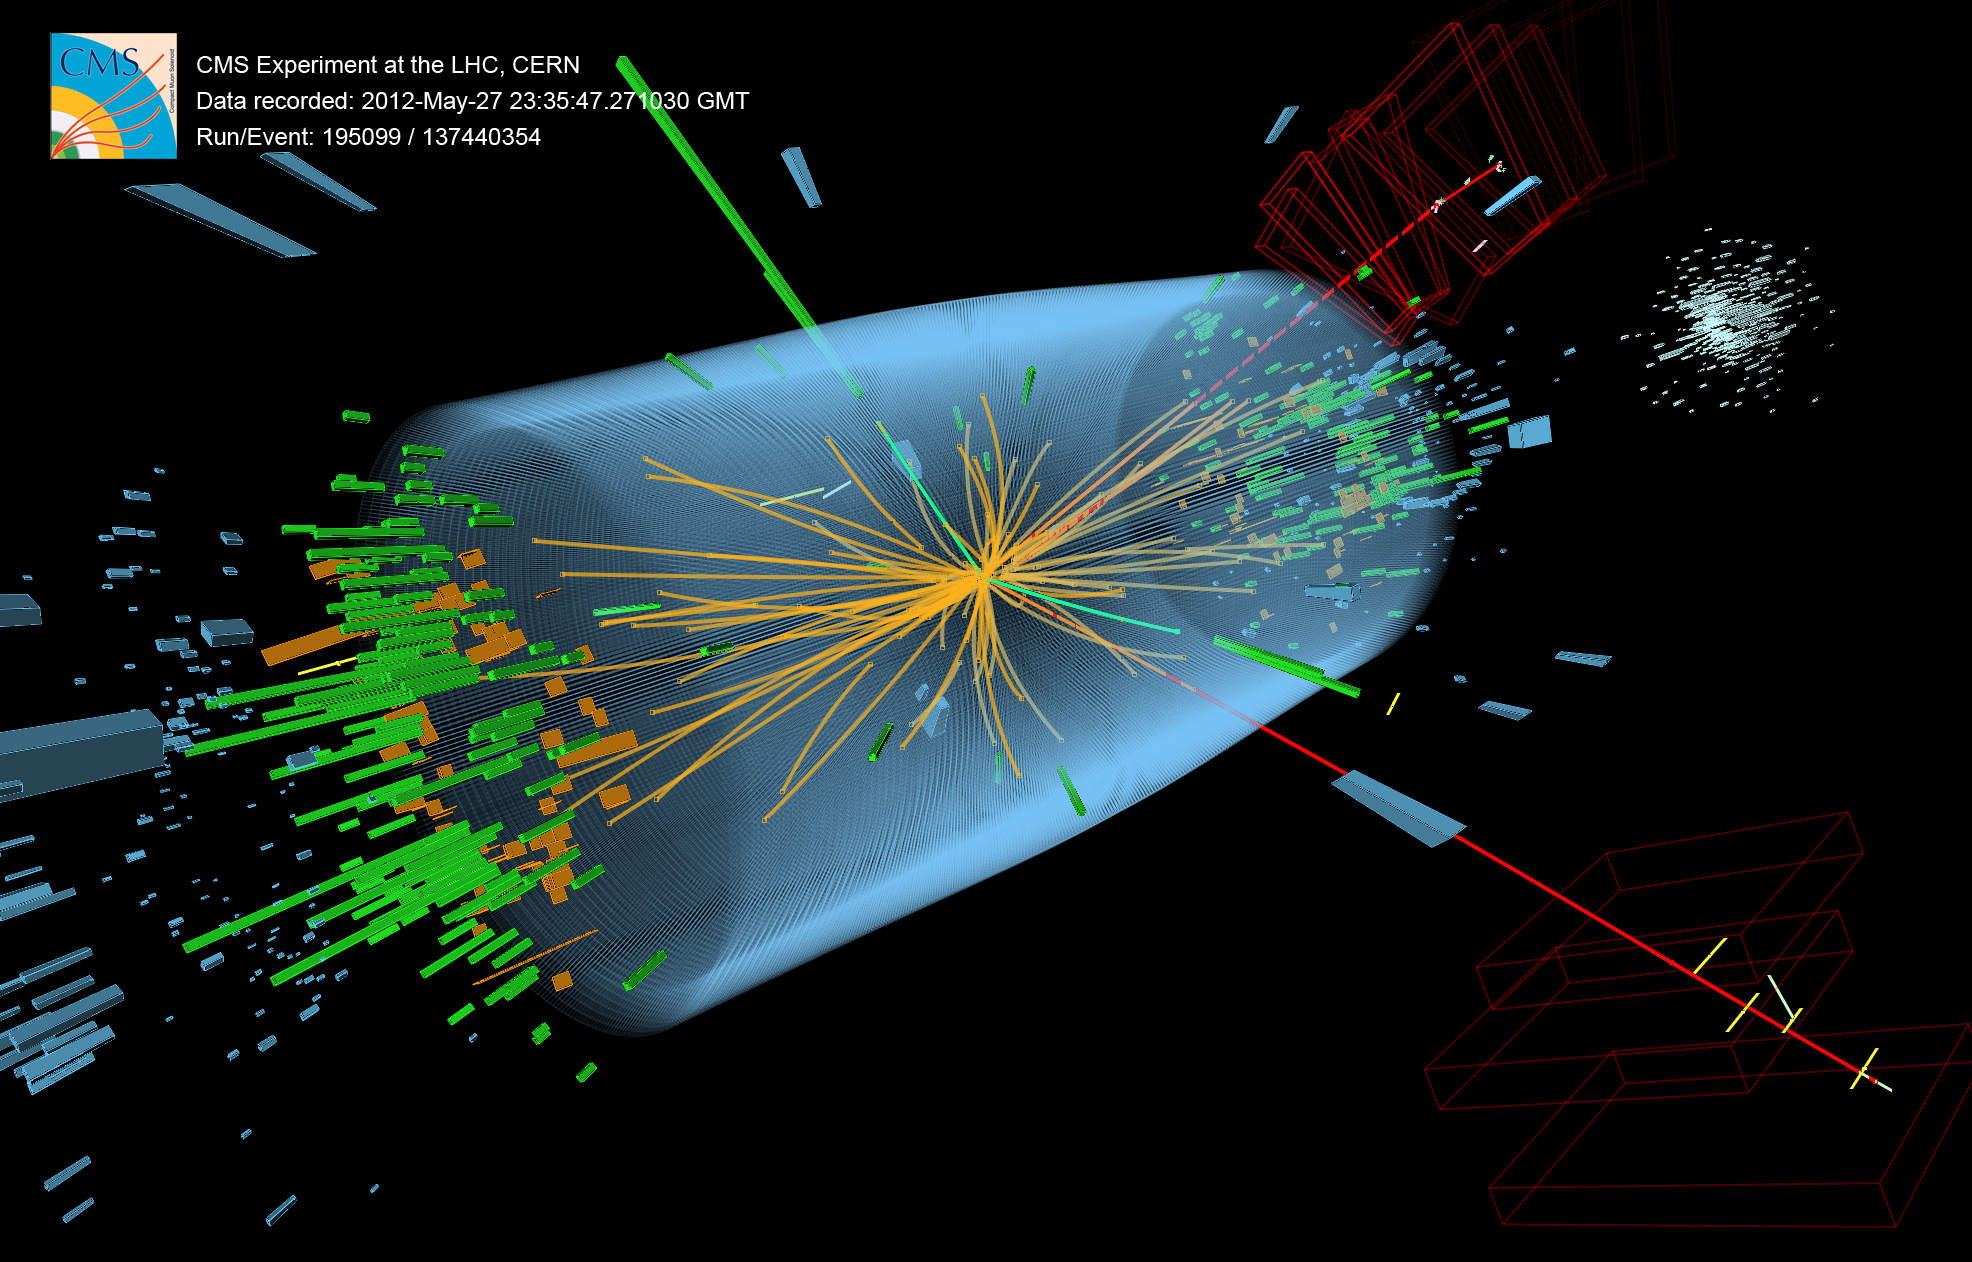
\includegraphics[width=\textwidth]{images/higgs}
%   \caption{Observed candidate decay of Higgs$ \rightarrow ZZ^\ast (ee\mu\mu)$,
%   where the green and red lines emanating from the center are two electrons and
%   two muons, respectively.\cite{higgs}}
%   \label{fig:higgs}
% \end{figure}

\begin{figure}
  \centering
  \begin{minipage}[t]{0.49\textwidth}
    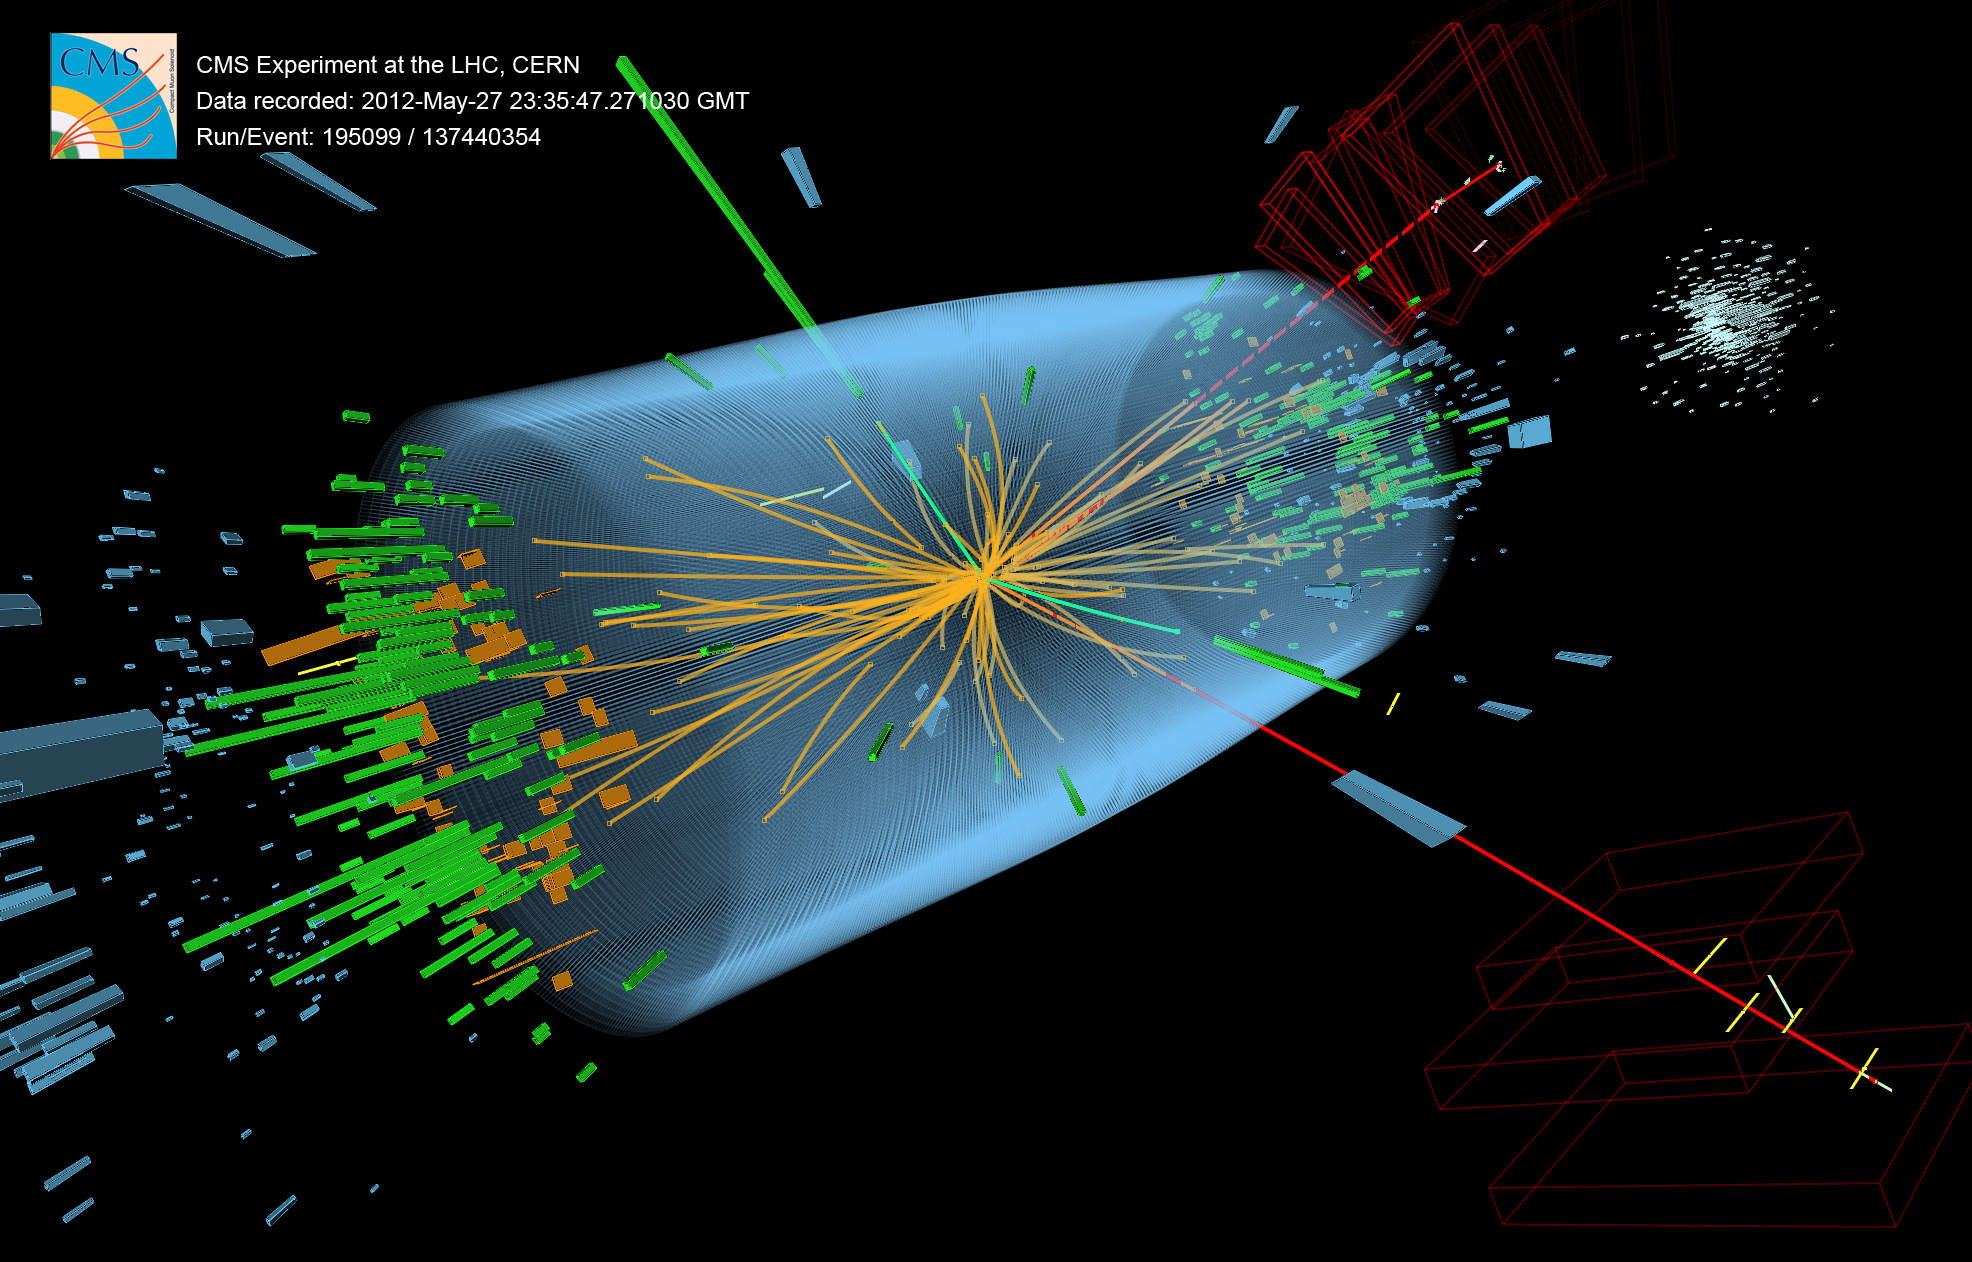
\includegraphics[width=\textwidth]{images/higgs}
    \caption{Observed candidate decay of Higgs$ \rightarrow ZZ^\ast (ee\mu\mu)$,
    where the green and red lines emanating from the center are two electrons and
    two muons, respectively.\cite{higgs}}
    \label{fig:higgs}
  \end{minipage}
  \hfill
  \begin{minipage}[t]{0.49\textwidth}
    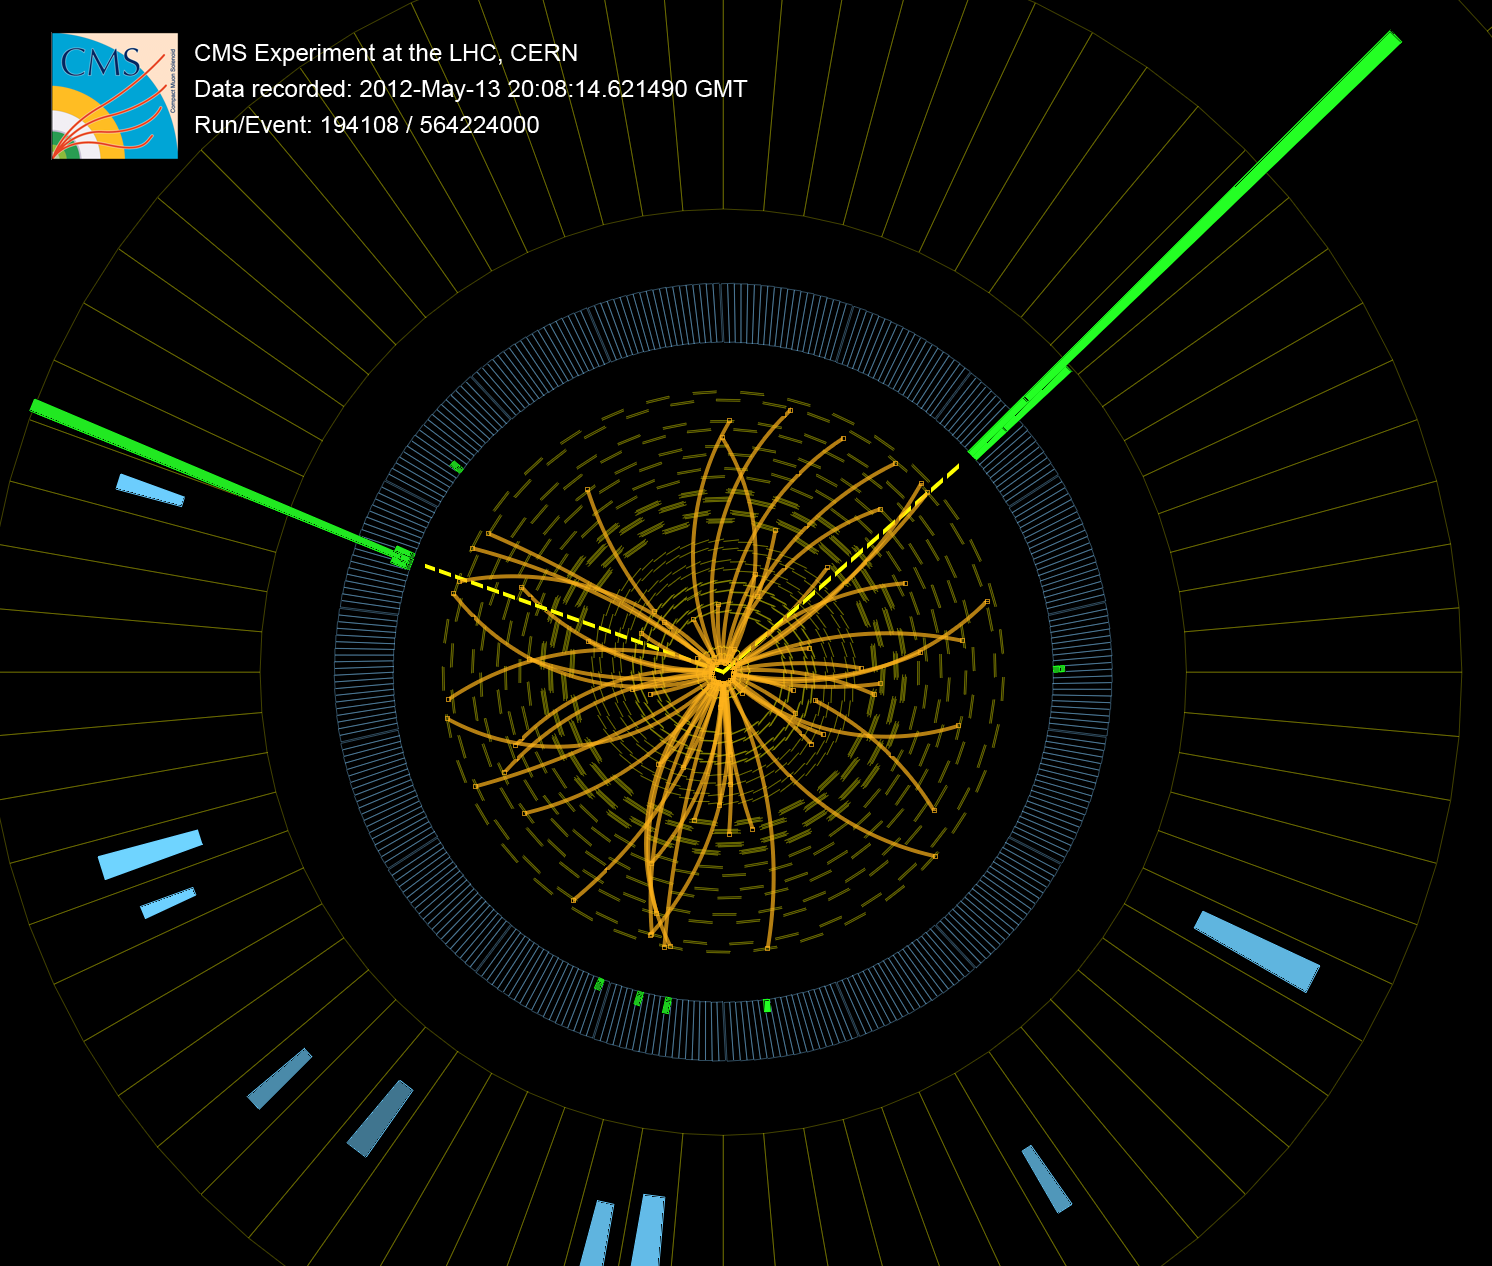
\includegraphics[width=\textwidth]{images/higgs2}
    \caption{Observed candidate decay of  Higgs$ \rightarrow \gamma\gamma$, the
    green lines eminating from the center are two photons.\cite{higgs2}}
    \label{fig:higgs2}
  \end{minipage}
\end{figure}

CMS is designed to be capable to observe particles resulting from proton-proton
collisions with a center-of-mass energy of $\sqrt{s} = 14$TeV produced by the
Large Hadron Collider (LHC).
Currently the LHC provides collisions with a center-of-mass energy of
$\sqrt{s} = 13$TeV.

More information about the LHC experiments can be found in the book
`The CERN Large Hadron Collider: Accelerator and Experiments`\cite{CMS_Experiment}.

\section{The structure of CMS}
\subsection{Silicon Tracker}
The tracker can reconstruct the path of passing muons, electrons, and charged
hadrons. Because it is closest to the collisions, the decays of very short-lived particles (e.g.
beauty quarks)\cite{aboutCMS} can be detected.

It makes very precise measurements on the location of particles (with an accuracy
up to \SI{10}{\micro\meter}). Accompanied by a magnetic field, the momentum of
these particles can be determined.
Yet this section tries to be as unobstructive to particles as possible. This is
accomplished by using a silicon microstrip design, minimizing the volume of material that
can obstruct particles.

Being the closest to the proton-proton collisions, this part of the detector is
the one that has to endure the most radiation.
\subsection{Electromagnetic Calorimeter}
The Electromagnetic Calorimeter (ECAL) is a set of 75.848 lead tungstate (\ce{PbWO4}) crystals
with a total weight of about 100 tonnes.

It is designed to stop and measure the energy of passing electrons and photons.

These crystals produce light in the form of electromagnetic photon showers (see image \ref{fig:cms_slice})
that are measured by photodetectors (either avalanche photodiodes or vacuum phototriodes).

These crystals are very radiation hard and can reverse their radiation damage when
kept in room temperature (during beam time they are cooled to 0.1\degree C).
\subsection{Hadronic Calorimeter}
The Hadronic Calorimeter (HCAL) is designed to detect hadrons (i.e. particles
produced of quarks) and gluons.

This part of the detector is organized in several layers of dense absorbing materials and scintillators,
a combination of steel and plastic, where the plastic produces a light pulse when a particle flows through it.

The fact that the HCAL is housed inside the solenoid is one of the biggest
differences between the ATLAS and the CMS experiment.
\subsection{Superconducting Solenoid}
The design of CMS had a high focus on achieving the highest possible magnetic
field. To achieve this CMS has been equipped with one large superconducting
solenoid, capable of generating a magnetic field of \SI{4}{\tesla}.

This allows for very precise momentum readings by analyzing the arcs of charged
particles. It also provides sufficient return flux outside
the solenoid to be used by the muon chambers (about \SI{2}{\tesla}).
\subsection{Muon Chambers}
Muons (and neutrinos) are the only particles that can pass the previously
mentioned sections without losing most (if not all) of their energy.

The loss of energy as a particle travels through matter is  described by the
Bethe equation (\ref{eq:bethe}). Because of the characteristics of Muons,
this equation states that muons will not
release much of their energy as they pass through material.

Combined with the fact that these particles have high mass, this makes them very difficult to stop.

\begin{equation} \label{eq:bethe}
- \left\langle\frac{dE}{dx}\right\rangle = \frac{4 \pi}{m_e c^2} \cdot \frac{nz^2}{\beta^2} \cdot \left(\frac{e^2}{4\pi\varepsilon_0}\right)^2 \cdot \left[\ln \left(\frac{2m_e c^2 \beta^2}{I \cdot (1-\beta^2)}\right) - \beta^2\right]
\end{equation}

% $- \left\langle\frac{dE}{dx}\right\rangle = \frac{4 \pi}{m_e c^2} \cdot \frac{nz^2}{\beta^2} \cdot \left(\frac{e^2}{4\pi\varepsilon_0}\right)^2 \cdot \left[\ln \left(\frac{2m_e c^2 \beta^2}{I \cdot (1-\beta^2)}\right) - \beta^2\right]$


Since muons can't be easily stopped, the muon chambers rely
instead on the strong magnetic field to measure the curvature of these charged
particles, and thereby measuring their energy.
The muon chambers are composed of three components, the Resistive Plate Chambers
(RPC), Drift Tubes (DT), and Cathode Strip Chambers (CSC).


\begin{figure}
  \centering
  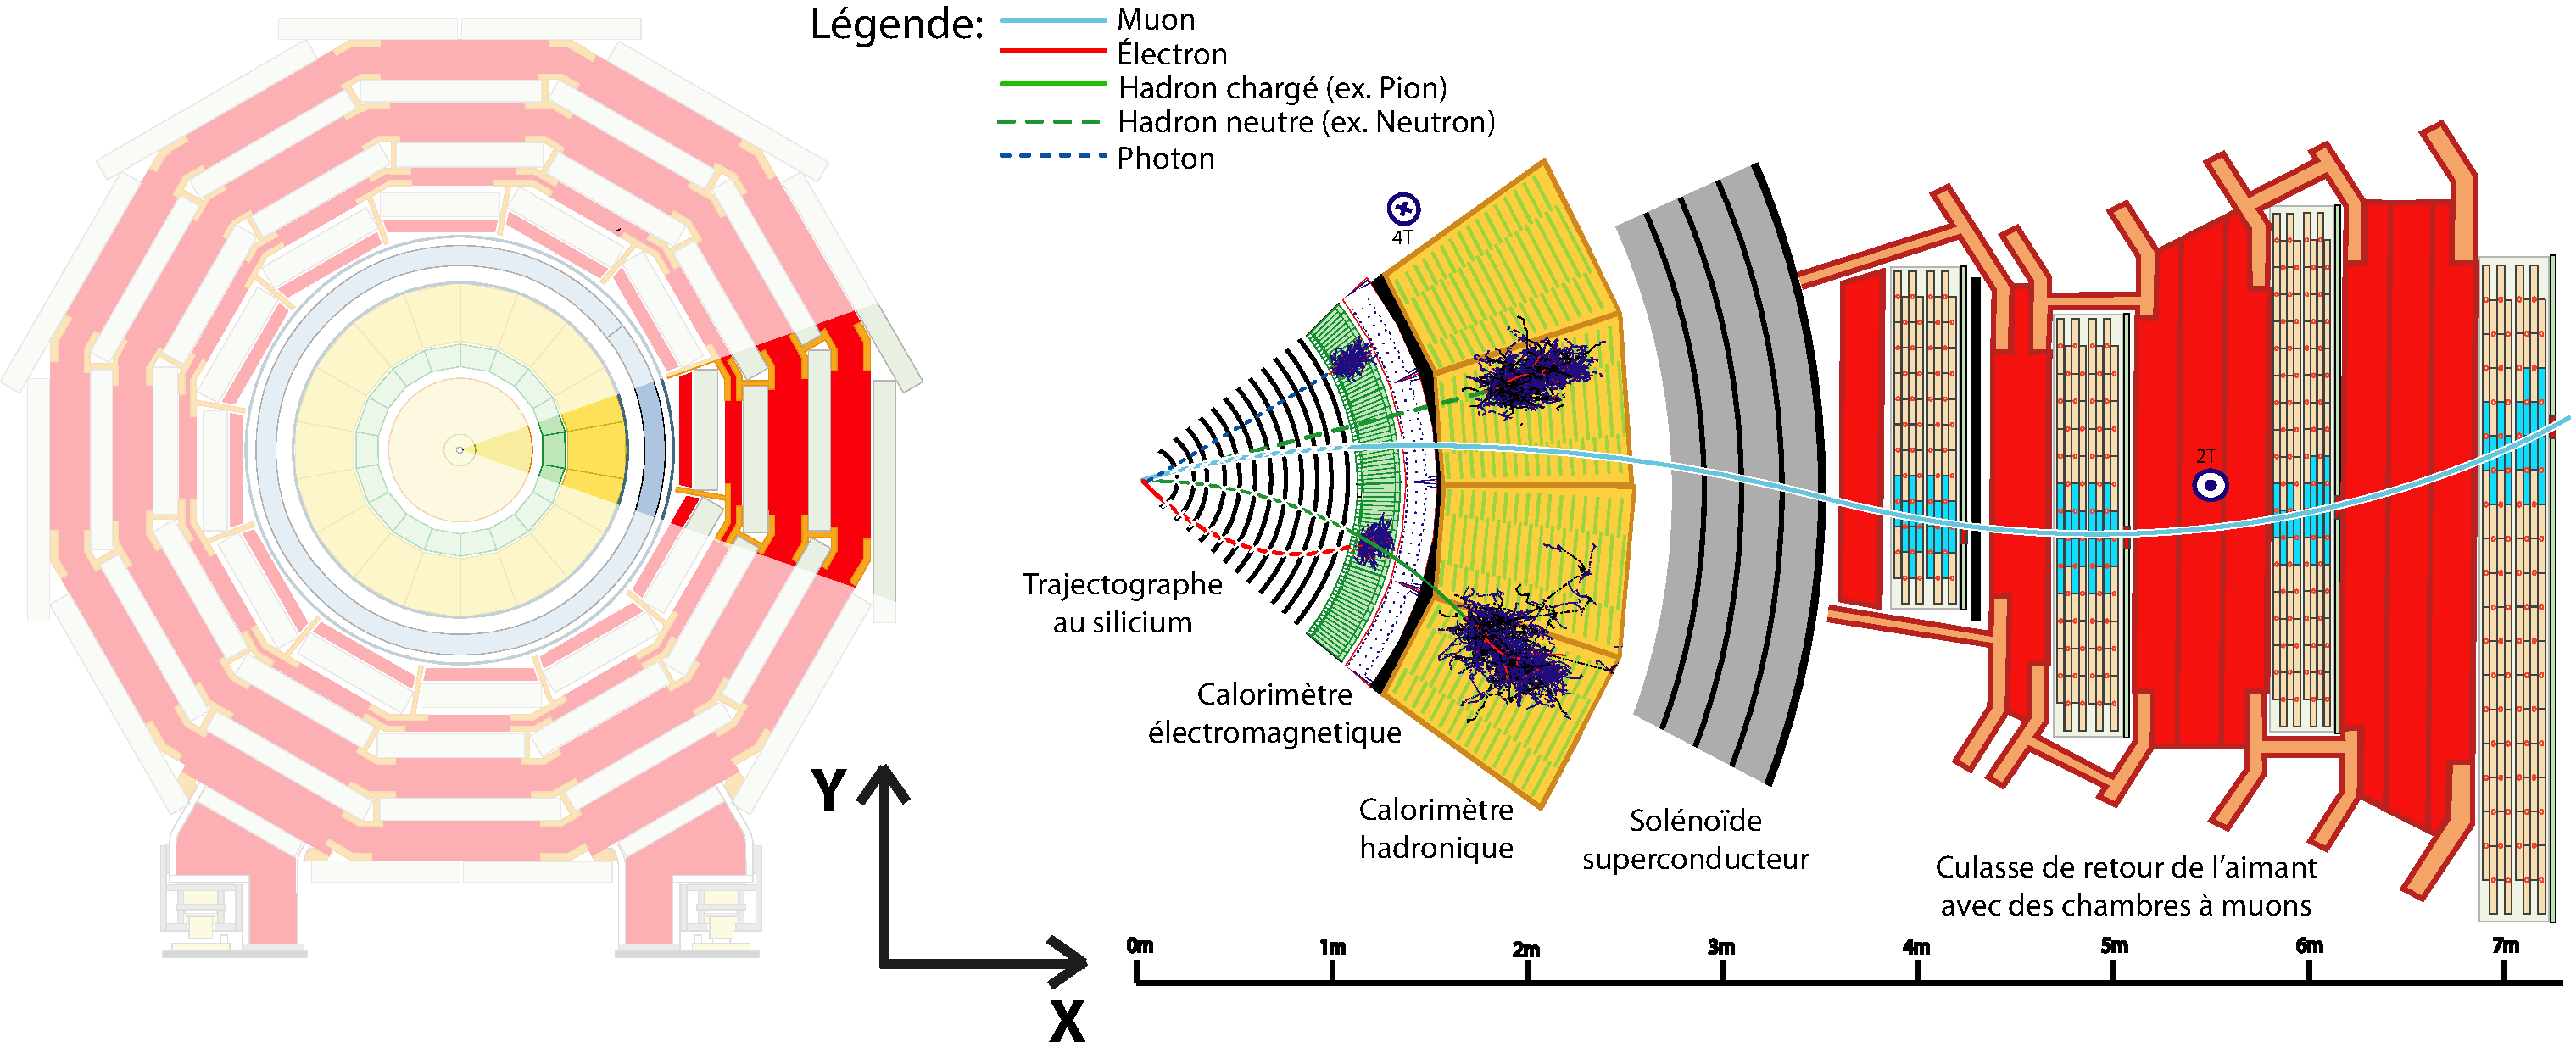
\includegraphics[width=\textwidth]{images/cms_slice}
  \caption{A transversal slice through the CMS detector, demonstrating the various
  sections of the detector and their designed functions.\cite{cms_slice}}
  \label{fig:cms_slice}
\end{figure}





% \section{The Level-1 Trigger}
% LHC produces proton-proton collisions in the center of the CMS detector. This is
% accomplished by providing a periodic moment bunch crossing in the detector.
% The LHC is currently designed to provide periodic bunch crossing in the detector
% at a rate of 40MHz and with a centre-of-mass energy of $\sqrt{s} = 14$TeV.
%
% The current luminosity of the beam in LHC will result in an average of ~40-50
% proton-proton collisions per bunch crossing, resulting in around 2MB of data
% generated by the sensor electronics.
%
% At a rate of 40MHz this will effectively produce a data stream of 80TB/s.
% This is too much for any storage system to handle, so a system is needed to
% filter this data so only data that looks interesting is retained.
%
% To handle this huge data stream, the level-1 (L1) trigger system is developed.
% Its purpose is to reduce the data stream to a maximum of 200 GB/s by filtering
% the collision rate to 100kHz.
% This reduction of data is done real-time and is programmed into field-programmable
% gate arrays (FPGAs) inside the detector.
%
% The bunch crossing frequency of 40MHz implies the L1 trigger has very little time
% to fully analyze a bunch crossing and decide which collisions to keep for further
% analysis.
%
% Currently, the time it takes for the L1 trigger to make a decision is \SI{3.2}{\micro\second},
% the time it takes for 128 bunch crossings to pass.
% Therefore all sensors have a buffer that can contain all the data of 128 bunch
% crossings. When the L1 trigger issues a L1 ACCEPT directive, the buffers are
% read and stored.
%
% This data is then passed to the high level trigger (HLT), to be further reduced
% to a 10 Hz collision rate.
% The high level trigger is also called the offline software because, unlike the
% L1 trigger, the calculations are not performed real-time.
% More information about the HLT can be found in the Phase II technical proposal
% \cite{TS_Phase2}.

\chapter{The Level-1 Trigger Online Software}
% read the paper about the cell structure
% - cell tree structure
% - web interfaces
% - panels \& SDK
% - Phase II plans

\section{The Level-1 Trigger}

The online software is designed to setup, configure, and monitor the electronics
responsible for analyzing and filtering data from the CMS experiment
as the LHC provides it with sets of proton-proton collisions in the center of
the detector at a rate of 40MHz.

The current luminosity of the beam in LHC gives an average of \~40-50
proton-proton collisions per bunch crossing, resulting in around 2MB\cite{CMS_Experiment2} of data
generated by the sensor electronics.

At a rate of 40MHz this will effectively produce a data stream of 80TB/s.
This is too much for any storage system to handle, so a system is needed to
filter this data so that only interesting events are retained.

To make the data rate manageable a set of (very fast) algorithms are executed on
hardware just outside the detector as events occur to filter out `uninteresting` data,
i.e. physics events that are already known and well-defined. This because
collision experiments have been performed for many years now and many observable
physics processes in them have already been thoroughly studied.

This filter is called the Level-1 (L1) trigger and will reduce the `event rate`
(i.e. bunch crossing containing proton-proton collisions) from 40MHz to a
relative rate of \~100kHz.

The output data stream of the L1 trigger is then forwarded to the high-level trigger
(HLT), which will reduce the event
rate from 100kHz to 100Hz. The output data from the HLT is then stored for
further analysis by the Worldwide LHC Computing Grid (WLCG).
More information about the HLT can be found in the Phase II technical proposal
\cite{TS_Phase2}.

The calculations of the L1 trigger are performed on FPGA (field-programmable
gate array) hardware.
These hardware boards follow a common firmware pipeline.
The L1 trigger is designed to make a decision every \SI{4}{\micro\second}, the
time it takes for 160 bunch crossings to occur.
The trigger will issue a Level-1 Accept (L1A) if this set of bunch crossings
is deemed interesting.

The trigger is composed of four levels.

The lowest level, called the Local Triggers or Trigger Primitive Generators (TPG),
is a set of hardware boards deployed in the calorimeters as well as the
muon chambers, where they are designed to analyze the energy readings and
recognize patterns.
This level contains the Electromagnetic Calorimeter (ECAL), the
Hadron Calorimeter (HCAL), the Cathode Strip Chambers (CSC), the
Resistive Plate Chambers (RPC), and the Drift Tube (DT).

The second level combines the information of the
Local Triggers and try to make basic reconstructions to determine what sort of
physics event has happened in that particular region of the experiment.
It outputs `trigger objects`, which signify the particle type (e.g. a passing electron or
muon) and a rank. The rank is determined by the energy, momentum, and a level of
confidence of this measurement.
This level contains the TwinMux, the Calorimeter Trigger Layer 1, the
Endcap Muon Track Finder (EMTF), the Overlap Muon Track Finder (OMTF), and the
Barrel Muon Track Finder (BMTF).

The third level, called the Global Calorimeter and Global Muon Triggers, filter
out the highest ranked trigger objects reported by the Regional Triggers.

The highest level, called the Global Trigger, determines whether or not to issue
a Level-1 Accept (L1A), and instructs the Timing Trigger and Control System (TTC)
to read out the full-precision data stored in the buffers of the FPGA hardware
inside the detector.
This level contains the Calorimeter Trigger Layer 2, the Global Muon Trigger ($\mu$GMT),
and the Global Trigger ($\mu$GT).

This trigger loop is explained visually in figure \ref{fig:l1triggerloop}.

\begin{figure}
  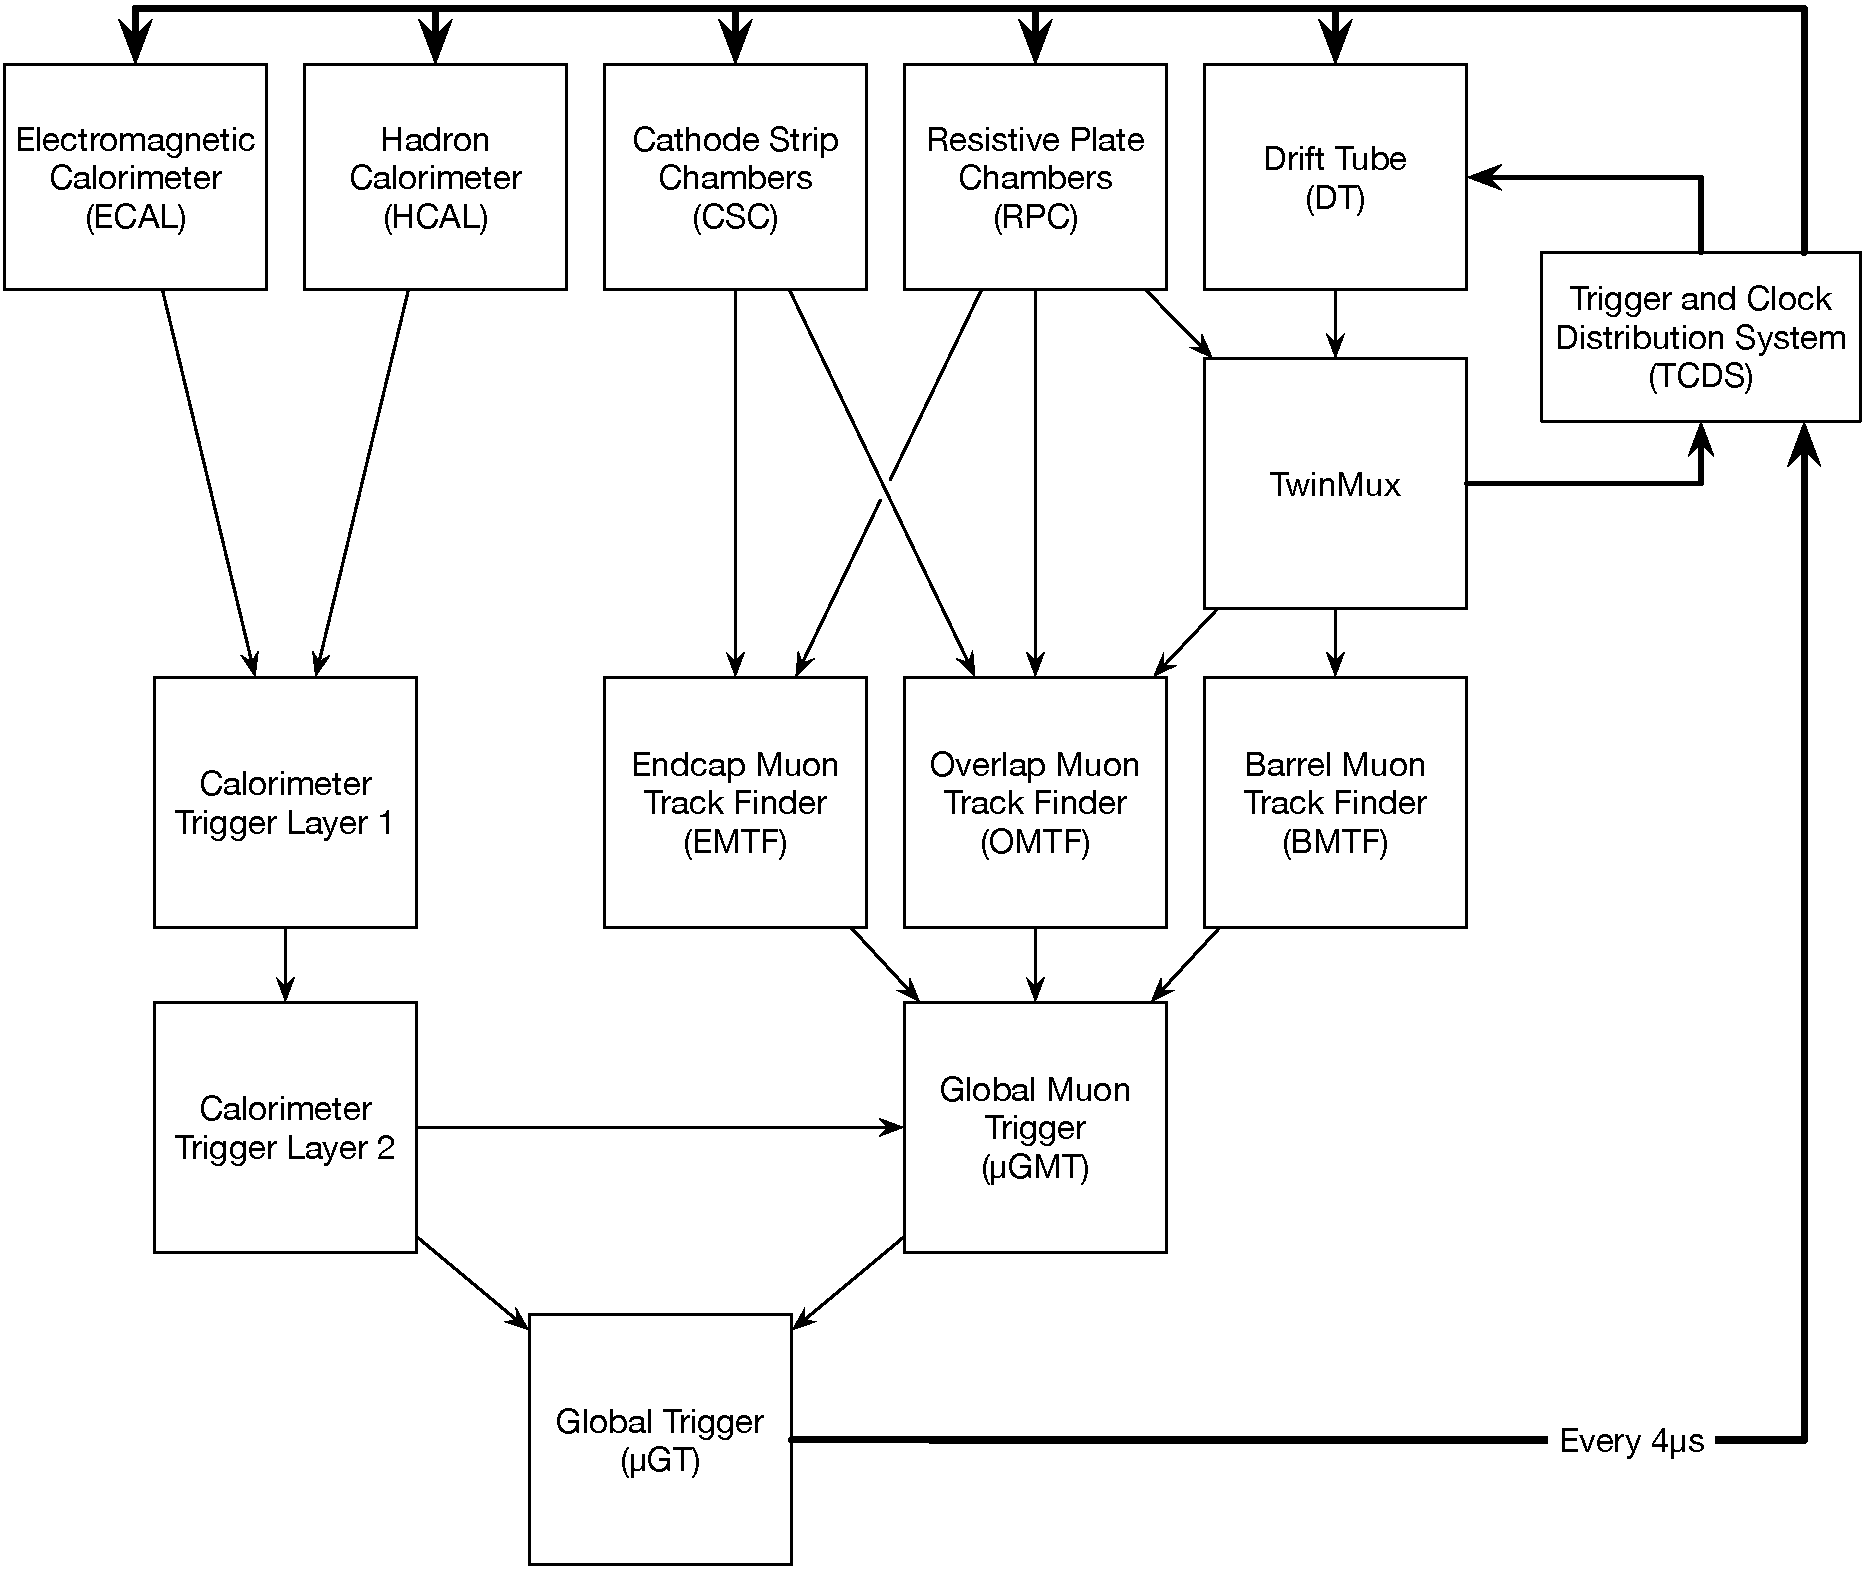
\includegraphics[width=\textwidth]{images/L1-trigger-loop}
  \caption{Conceptual drawing of the L1 trigger hardware loop}
  \label{fig:l1triggerloop}
\end{figure}

Note that, because of the decision deadline of \SI{4}{\micro\second}, the
buffers will contain data of 160 bunch crossings.

Also note that this trigger loop only considers data from calorimeters and
muon chambers to limit the data flow through the pipeline.

The Trigger and Clock Distribution System (TCDS) is in charge of distributing a L1A
and control signals (e.g. calibration, clock synchronization, test, reset, \ldots).

\section{The CMS Experiment Control System}
The CMS Experiment Control System (ECS) is a distributed software system that
is designed to manage the configuration, testing, and monitoring of all hardware
involved in the L1 trigger and DAQ system of the CMS experiment.

One of the components of ECS is the Cross Data Acquisition System, called XDAQ.
It is a custom-made data acquisition system specialized for high energy physics.
It is developed internally by the CMS group.

% It's task is to receive fragmented data about a collision event and reconstruct
% it to restore the full event.

XDAQ provides a standardized way to perform high energy physics analyses. It
provides developers with a uniform DAQ system. It hides the complexity of data
exchange and distributed computing for the developer.
It allows subsystems to load its own software modules to perform various tasks.
XDAQ also provides an interface engine each subsystem can use to render a web
interface.

\section{The Trigger Supervisor}
The Trigger Supervisor is a framework built upon XDAQ which specializes in
controlling the various aspects of the L1 trigger and providing libraries for
the execution of common tasks performed in most of the subsystems (e.g. configure, test, \ldots).
For example it provides standardized APIs for executing configuration commands and
generating monitoring data.

This composes a central system through which the status of all the subsystems
of the experiment can be monitored.

The Trigger Supervisor is, as it is built on top of XDAQ, distributed.
It is implemented in the form of a tree of `cells`.
The Trigger Supervisor has a root cell, called the Central Cell, which has
several subcells, each corresponding to a L1-trigger subsystem.
Each subcell can contain further subcells. A cell can be a hardware component,
or a controller. In the cell tree, all end nodes of the tree are hardware components.

Each cell creates its own web interface dealing with that cell's particular
functionality. This way a user can use the web interface to receive a general
overview of a system, and traverse the tree to get more specific data and
functionality.

\begin{figure}
  \centering
  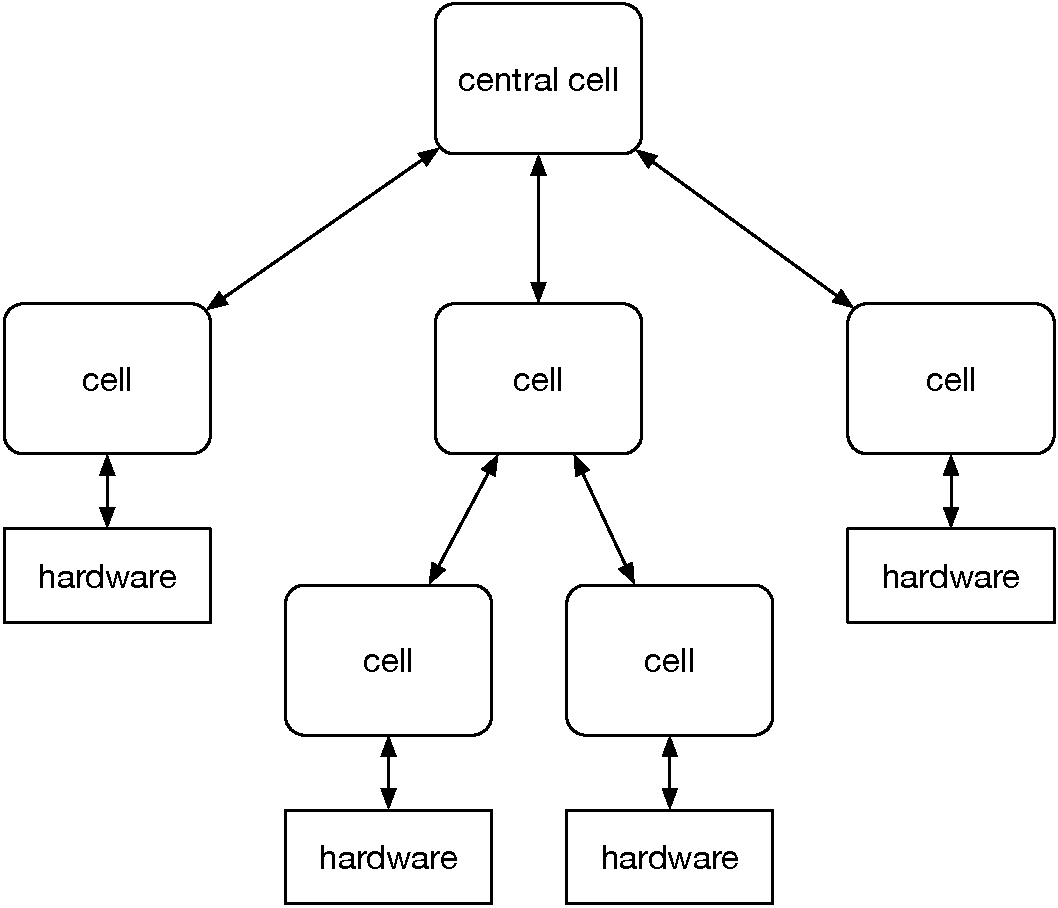
\includegraphics[width=.75\textwidth]{images/cell-tree}
  \caption{An example of the Trigger Supervisor Cell structure}
  \label{fig:cell-tree}
\end{figure}

\section{SWATCH}
The phase II upgrades of LHC will increase the luminosity of the produced beams.
This means there will be more proton-proton collisions per bunch crossing in the
experiment, which in turn means there is a bigger amount of data that needs
processing.

To support this increase of collision rates, the current hardware at CMS needs
to be adapted or replaced to support the higher data rate.

The SWATCH project (SoftWare for Automating conTrol Common Hardware) is an
endeavor to standardize the communication with boards and the functions they
provide.
It attempts to exploit commonalities between hardware components and uses it
to provide a common high level API to greatly simplify the development of the
online software\cite{SWATCH}.

\chapter{Problems with TS 2.0}
\label{Problems with TS 2.0}
The Trigger Supervisor version 2.x had a few problems that caused
frustrations with both the operators and the developers of the software.

\section{Browser compatibility}
The first and most visible issue is the slow degradation of support for the
interface in modern Web Browsers.

This is due to an effect caused by the movement of major web browser vendors to
become `evergreen`, which started around 2011.

\subsection{Evergreen browsers}
\label{Evergreen browsers}
An evergreen browser, in essence, is a browser that updates itself without the
interaction of the user.
This is the formal definition of an `evergreen` browser, however there are
some new philosophies that come with this approach.

First off, a web browser's version number no longer has a real meaning.
To a user a web browser will now be `versionless`, the user will no longer know
nor care what browser version is running and will actually assume it is the latest
version.
Browser vendors have combined auto-updating with a significant speedup of their
release cycles. Browsers now tend to update their version once a month, rather
than at most once a year (see figure \ref{fig:updateGraph}).

This corresponds to the release early, release often (RERO) software design
philosophy. An approach popular in the open-source community and used for the
development of the Linux kernel\cite{TheCathedralAndTheBazaar}.

\begin{figure}
  \centering
  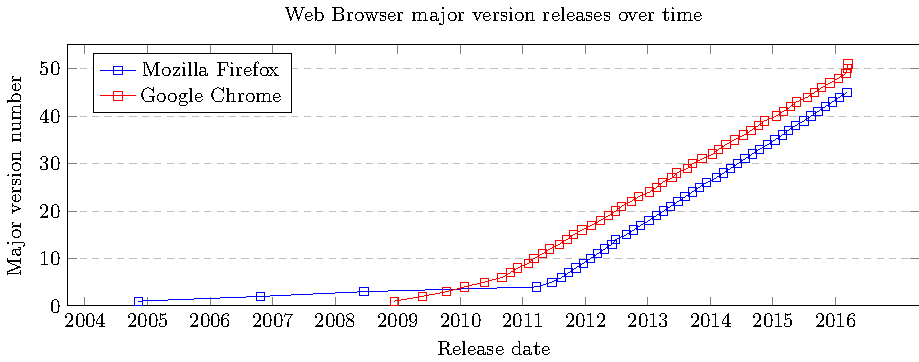
\includegraphics{images/pgfplots/firefox_update_speed-figure0}
  \caption{Overview of major version releases of Mozilla Firefox and Google Chrome over time}
  \label{fig:updateGraph}
\end{figure}

This in turn engaged web browser vendors to implement new standards much faster
and in a much more iterative way than previously possible.
Web browser vendors will no longer develop new features as a whole, but rather
slowly implement a feature piece by piece.
A good example of this is ES6 (sometimes called JavaScript 2015). ES6 is in
essence a set of extra JavaScript functionalities and additions to the syntax.
Without evergreen browsers, this would have been implemented as one big update,
probably in the form of a major release update.
However, evergreen browsers implement every ES6 feature bit by bit. This can be
tracked with the ES6 compat-table project\cite{compattableproject}.

Because of these rapid release cycles and automatic updates, evergreen browsers
introduce a change in behavior of keeping compatibility with older webpages.
If a particular feature would inhibit the development of new features or what is
sometimes referred to as `moving the web forward`, it has become acceptable to
completely remove that feature.
The latest example of this behavior can be found in the rapid implementation,
and equally rapid removal, of the /deep/ and ::shadow CSS selectors\cite{deepAndShadowCSS}.
This goes against the previous philosophy that a web browser must maintain
backwards compatibility with older web pages as much as possible. And this is
the main reason the TS 2.0 interface is experiencing problems with modern browsers.

\subsection{Interface degradation}
\label{Interface degradation}
The age of the TS interface (8 years as of this writing) has reached a point where it
uses HTML, JavaScript, and CSS that is being actively removed by browsers.
This gives some potentially serious issues when operating the interface.

The most prominent example is the modal dialog feature of the interface.
In Mozilla Firefox version 38, the one currently installed in the CMS Control
Room, the modal dialog behaves fine. A white overlay is put over the interface
and a dialog appears, forcing the user to take a decision.
However in the latest version of Firefox, currently 44, the dialog does not appear
while the white overlay does appear. This effectively blocks the user from using
the interface at all from that point and forces a page reload.
Whatever functionality was implemented using the modal dialog is now inaccessible.
See figure \ref{fig:ff38} and \ref{fig:ff44}.
\begin{figure}
  \centering
  \begin{minipage}[b]{0.49\textwidth}
    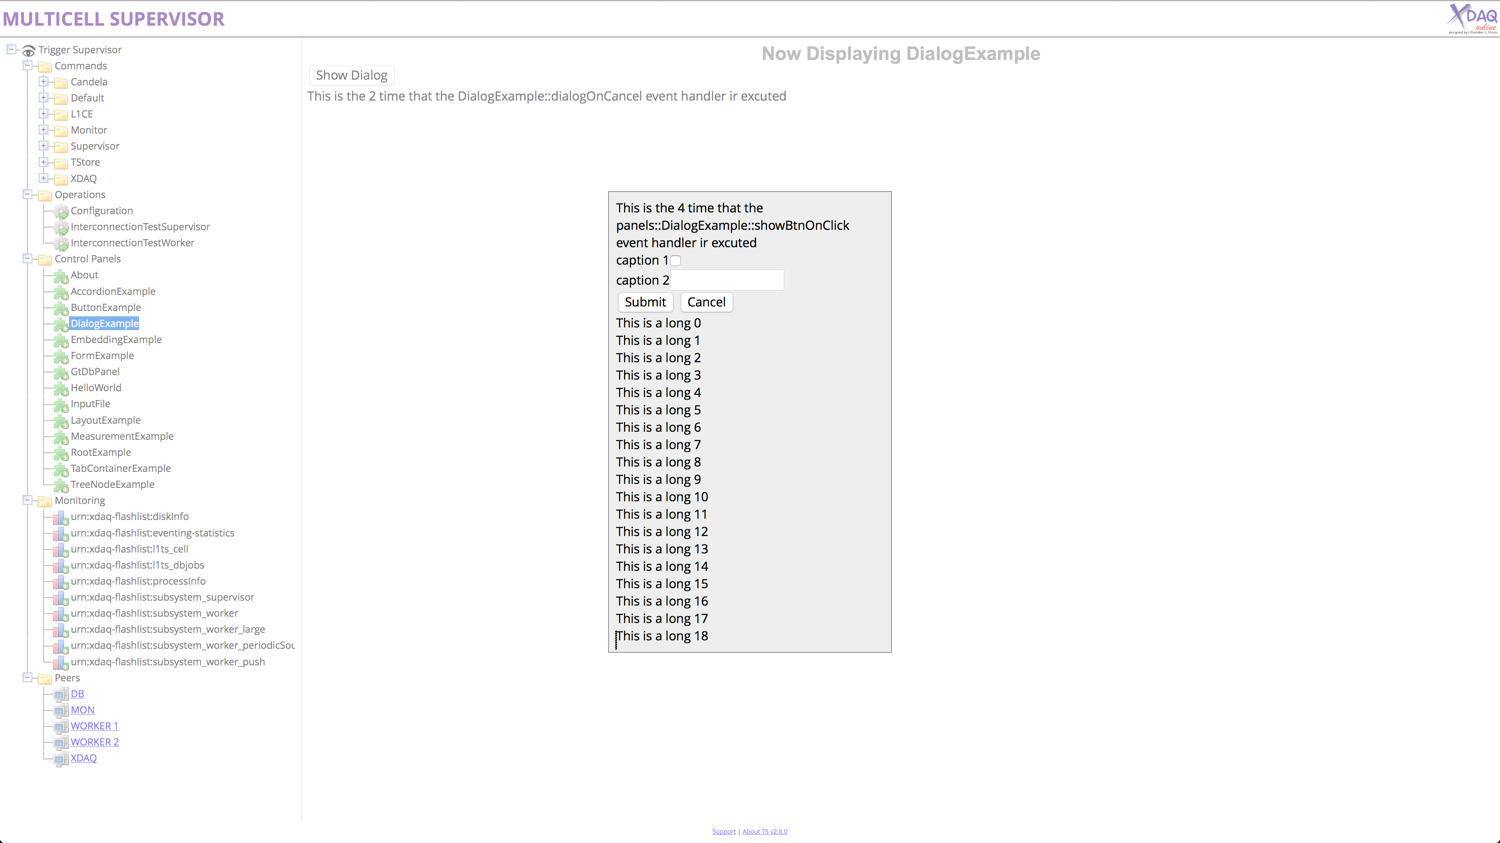
\includegraphics[width=\textwidth]{images/modal_ff38}
    \caption{The modal dialog in Firefox 38}
    \label{fig:ff38}
  \end{minipage}
  \hfill
  \begin{minipage}[b]{0.49\textwidth}
    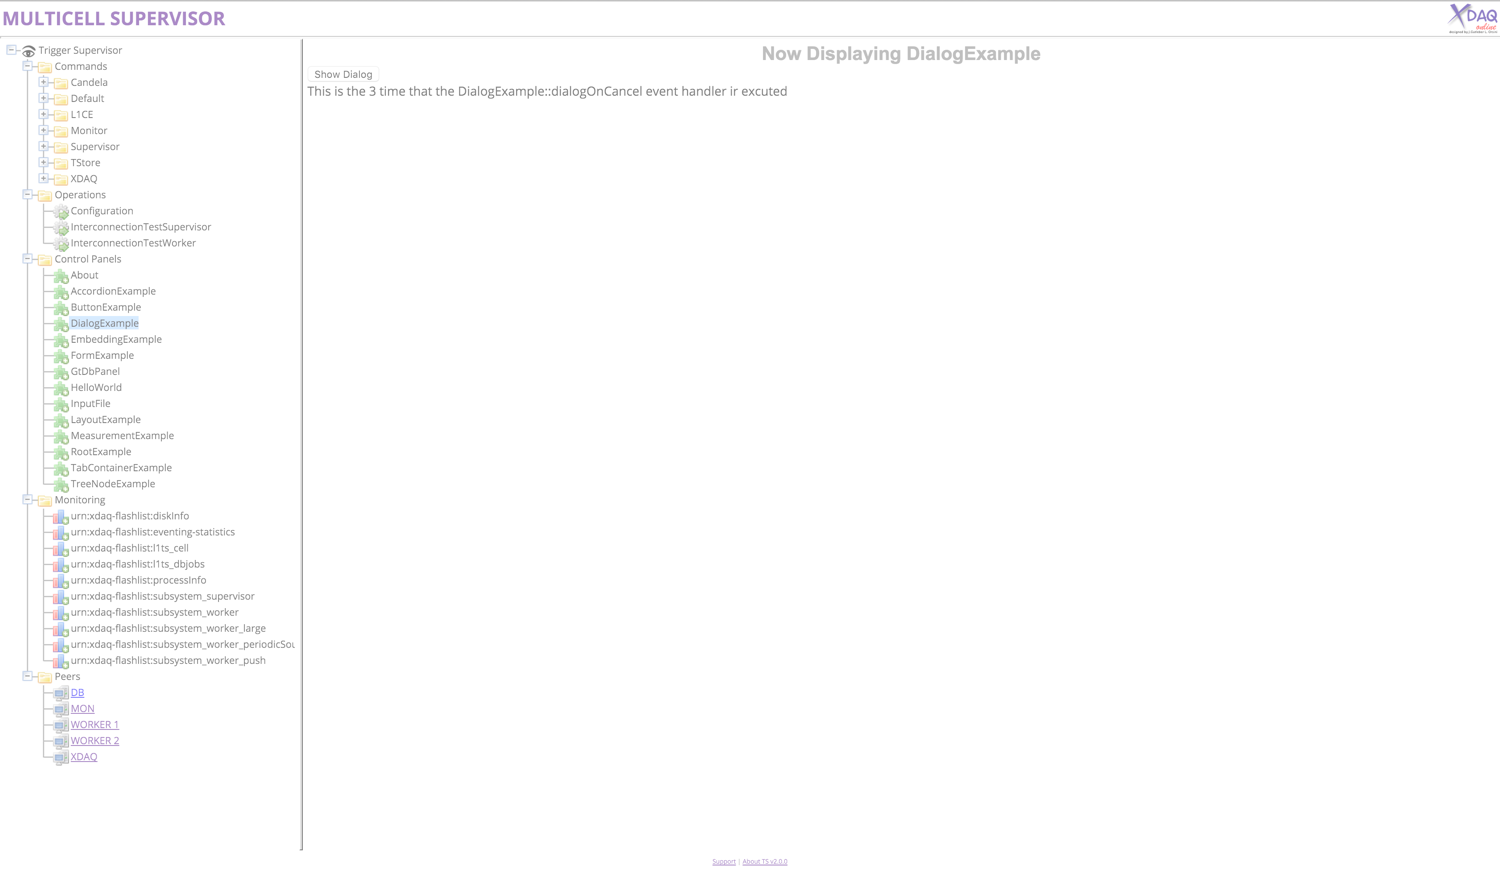
\includegraphics[width=\textwidth]{images/modal_ff44}
    \caption{The modal dialog in Firefox 44}
    \label{fig:ff44}
  \end{minipage}
\end{figure}


\begin{figure}
  \centering
  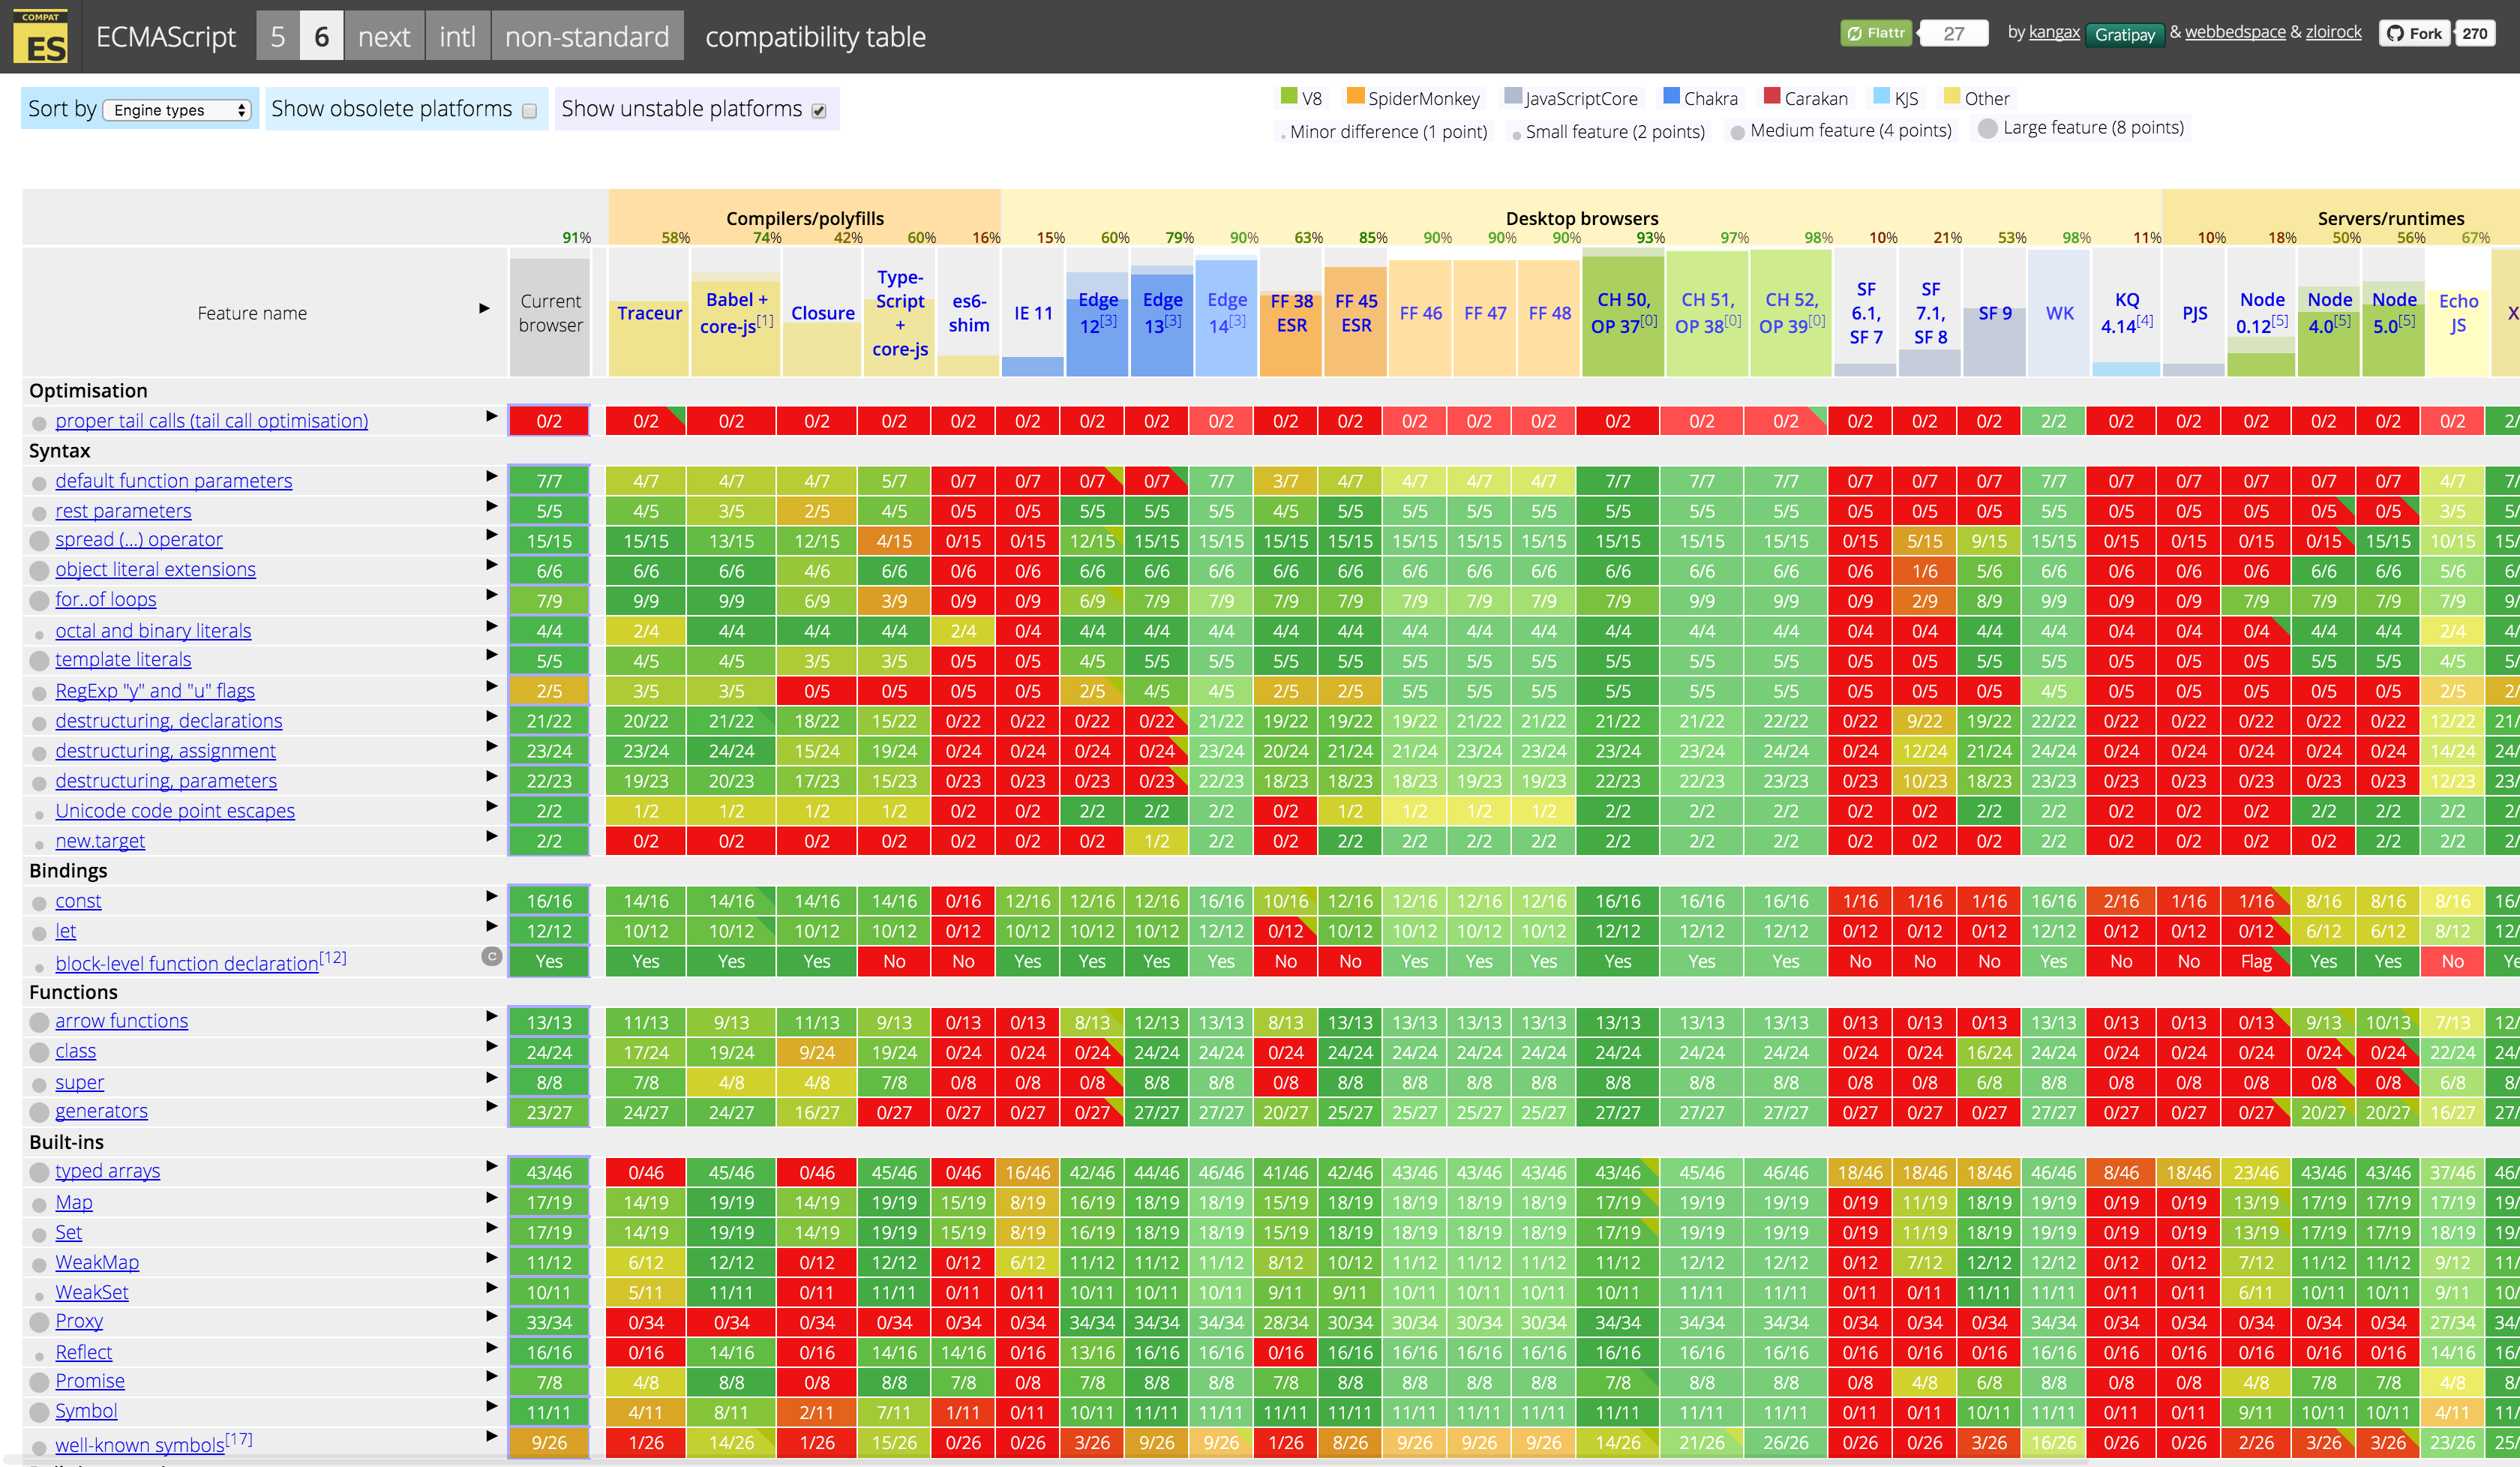
\includegraphics[width=\textwidth]{images/compattable}
  \caption{The ECMAScript compatibility table project}
  \label{fig:compattable}
\end{figure}


CERN uses only Extended Support Releases (ESR) of Firefox, and fortunately in
this case Firefox ESR deployments at CERN are always about a version behind on
the most up-to-date ESR release.
This means the interface degradation is currently not breaking functionality yet,
however it will in the near future and must be addressed as soon as possible.

\subsection{Dojo 0.4}
The front-end JavaScript framework used to render the interface is called Dojo.
It was one of the first JavaScript libraries that successfully attempted to extend
the standard html primitives and one of the few frameworks that worked fully
client-side.

It was very innovative to pick this framework for the first version of the TS.
However, as the version number suggests, it is a beta version. It has some flaws,
one of them being a rather huge memory leak issue (discussed in chapter \ref{Memory-leak problem}),
another being the ever increasing development time when building interfaces with
Dojo 0.4.

\section{Increasing development time}
Dojo 0.4 is around 8 years old now, developed in 2008\cite{TS_PHD}, it cannot be expected to
satisfy modern web application requirements.

It misses helper components to set up a layout, something every modern web
framework has nowadays, and forces the developer to reinvent the wheel
continuously when it comes to interface layouts. This is one of the big reasons
interface code tends to become huge and nigh unreadable.

\fvset{frame=single}
\begin{pyglist}[language=cpp,numbers=left,numbersep=5pt,fontsize=\small]
<!-- A simple title must be coded manually. Prone to typing errors (h2/h4) -->
ajax::PlainHtml* title = new ajax::PlainHtml();
title->getStream() << " <h2 style=\"font-family:arial; color:grey;\"" <<
" align=\"center\">Measurement Example</h4>" << std::endl;
add(title);

<!-- styling must be done manually -->
result_ = new ajax::ResultBox();
result_->setId("subsystem_btnpanel_result_");
result_->set("style","margin:20px; padding:20px; border:2px solid; ");
add(result_);

<!-- some panels need confusing styling to be functional -->
ajax::AccordionContainer* ac = new ajax::AccordionContainer();
ac->set("style","height:80%; width:80%;");
add(ac);
\end{pyglist}
\fvset{frame=none}

It also misses features that cannot be easily compensated. As the requirements
for the Phase II upgrade brings increased complexity, it will translate in the
framework's need to be able to handle increasing amounts of data reliably.
Think for example about large data tables that need filtering and sorting and
manipulation while at the same time keeping memory pressure low.

The current framework simply cannot supply this. And all attempts have resulted
in an ever increasingly slow interface and complexity in use.
For example, an attempt has been made to renew the `operations` interface.
This is an interface that controls a Finite State Machine (FSM) and allows an
operator to direct the flow through this FSM and input configuration parameters
for each transition.
This has been worked on for three months, but was eventually scrapped awaiting
the new TS release and it's new ways to develop interfaces.

\subsection{Maintainability}
The fact that simple tasks take much code to implement, combined with the
ever increasing complexity required from the interface, results in a
maintainability problem. Code becomes unreadable and even small code adjustments
take weeks to implement. Larger tasks or new functionality usually are even more
challenging to implement.

A recent functionality addition that actually made it into release was the ability
to download an arbitrary file from the server.
The requirement was to have a download button next to the text area that already
contained text of the file that would be downloaded.

It took three different approaches to downloading a file, each implementation
more inappropriate than the other. But finally a solution was found, where the file source
is just displayed in a new window, allowing for the user to right-click and
select `download source`.
Any standard or commonly used way to provide downloading of files ended up being
impossible to reliably implement because of the age of the framework TS 2.0
operated on.

This provides another point on why a change was needed.

\subsection{Large input problem}
\label{Large input problem}
The Dojo 0.4 framework uses HTTP GET requests with parameters encoded in the url
to make requests and post data to the cell.
This has some issues one of which recently became a big problem.

First off, HTTP GET, PUT, and DELETE requests should be idempotent. This means
that 2 identical requests at different times must produce identical results.
Not following this principle creates issues when a proxy server is between the
client and the server. A proxy server will always try to cache requests that
are supposed to be idempotent.
Some HTTP headers exist that allow a developer to instruct a proxy server to not cache
a particular request, but it is up to the proxy server implementation to decide
if such a request will be honored, and thus cannot be relied on.

Every request currently has such `no-cache` HTTP headers. And, luckily, no issue with
proxy servers has come up yet, however some browser issues are suspected
to be linked with this issue.

The second issue is the fact that the parameters of every request are url encoded.
This means that parameters are added to the url in the following fashion:
\begin{lstlisting}
http(s)://host:port/path?parameter1=value1&paremeter2=value2
\end{lstlisting}
The problem with this is that there is a maximum length the url is allowed to be,
the exact maximum length depends on both the used browser and server software.

The general consensus is that URLs should be kept under 2KB in size and must not
exceed 8KB, as this is where most browsers and server software draw the line.
Some panels however, like the operations panel, are
designed for very large input variables and far exceeded these limits.

This used to be fine with version 12 of the server software (XDAQ), but in the
recently introduced version 13, a hard limit of 8KB has been introduced.
This breaks important use cases of panels. It is technically possible to change
the Dojo framework's code regarding request handling. However this might
present unforeseen consequences given this is a rather low-level change. Rather
it has been decided TS 2.0 will never run under the new XDAQ 13 version.

\chapter{TS 3.0 upgrade requirements}
The previous chapter discussed the problems with TS version 2.0.

It is desirable to mitigate all these problems and prepare TS version 3.0 for
the future.
Several requirements were submitted to the then hypothetical new TS 3.0
components.

\section{Legacy code compatibility}
Currently there are many panels developed in the legacy TS. It is unfeasible to
upgrade or rewrite these all in one go. There will be a transitional period where
legacy code will have to run concurrently with newer code.

Therefore TS 3.0 must maintain as much code compatibility with TS 2.0 as possible.
It is very desirable to have 100\% compatibility. A slight area of code
incompatibility might have large consequences depending on legacy panel code.

This will put some restraints on the upgrade options as full legacy code
compatibility requires the new codebase to be a superset of the old one.
However this constraint is mostly applicable only to the server side code, as
the client side code is generated by the server and can be significantly
modified provided developers keep watchful of any changes.

\section{Ability to migrate code}
As the legacy code will be converted to new code, it would be desirable to
make the transition as easy as possible and not to have a too much difference
between modern and legacy code as far as keeping existing functionality is
concerned.

New functionality will of course result in new code. This requirement therefore
only applies to migrating legacy code to keep the functionality as it was.

\section{Future proof}
Web technologies are moving forwards in a fast pace. A lot of new standards have
arisen for us to use and it would be wise to use them.

Designing a codebase that uses as much open standards as possible is a good
practice. It ensures good support from communities using those standards, and
ensures the codebase will maintain compatibility with web browsers for a far
longer period than would otherwise be possible.

Provided finalized open standards are used, it would be acceptable to use
relatively modern technologies and currently heavily rely on polyfills, libraries
designed to emulate a spec not yet implemented, to provide the needed
compatibility with currently used software.

\subsection{Polyfills}
A polyfill is a term used in web development. It is a group of JavaScript
libraries designed with the very specific use case to implement a future
standard, or even just a working draft of a standard, as accurately as possible
with today's resources. Some of these also seek to fix a broken implementation
of a standard by specific browsers.

Polyfills have gained a lot of popularity the last few years, approximately in
tandem with the upcoming of `evergreen` browsers, as web development now mainly
focuses on building on open standards rather than focus on a specific browser
or even a specific version of a browser.

Polyfills are generally allowed to introduce as much CPU, memory, and network
usage as needed to implement their targeted standard as completely as possible.
The main argument for this is that a polyfill is designed to be obsolete after
web browsers have caught up and implemented said spec. At this point a polyfill
is designed to no longer be activated anymore, mitigating the originally
introduced loads.

\section{Rich functionality}
One of the main reasons to renew the codebase of the TS is to be able to fulfill
the new modern requirements for the interface.

A lot of new features are needed, like the ability to handle large datasets and
the ability to handle more complex analysis use cases.

It would be desirable to have an extendable framework. This way, as time goes on
and requirements change, the framework can be adapted and extended to handle
new requirements as needed.

\section{Faster development}
The new framework must be much faster to develop on, as currently it takes weeks
to implement any change whatsoever.

The current main inhibitors of development time are the lack of features and
the amount of unreadable code that the use of the framework causes.

Given the main problems of the slow development time it can be expected that,
whatever the new framework looks like, will introduce a major improvement of
development time of new interface panels.

\section{Stability}
The new codebase will have sessions at the CMS Control Centre that last for days.
This puts important requirements on front-end libraries and frameworks.

Memory leaks are unacceptable. A memory leak results in an unstable interface,
which is unacceptable during operations in the Control Centre.
This is explained in more detail in chapter \ref{Memory-leak problem}.

\section{Reduced code footprint}
The current code of an interface panel is too large and too messy.
It makes the code unreadable and very difficult to maintain.

It would be desirable to have a far smaller code footprint for basic panel
functionality. It is a sign of a more powerful framework and will ease the
later modifications to panel code.

A smaller amount of required code would translate to the need for a more powerful
framework. It must however not introduce functionality that abstracts
away it's functionality so much that it would introduce `black magic` code, i.e.
code that works but nobody knows why\cite{jargonfile}.

\section{Better maintainability}
Functional requirements change regularly. Whatever the new framework looks like
must be flexible and open enough to be extended or modified to provide for new
functionality as needed. This must either be done in-house or by an extensive and
stable developer community associated with the framework.

A `dead` framework, i.e. one that has no more developer community or ability to
be easily modified in-house, like happened with Dojo 0.4 must be avoided.

\section{Better documentation}
The previous requirement of maintainability puts a strong emphasis on documentation.
A system can't be properly maintained, nor modified, if the system's workings
aren't properly explained.

The framework will need extensive documentation describing the possible ways to
program panels and showcase advanced functionalities.
Documentation must also exist about the inner workings of the framework.

Documentation must also be easily kept synchronized with the actual state of the
code. This would suggest the use of inline documentation, i.e. documentation that
resides in the source code.

\section{i18n}
Given the multilingual environment this framework will be used in, it is
useful to have a codebase that can adapt to different interface languages.

\section{Browser compatibility}
The TS 3.x front-end libraries must be able to operate on CERN supported browsers.
This means it must support any browser installed by default on the currently
supported CERN Virtual Machines (VMs). Currently this is Scientific Linux CERN 6
(SLC6) (\url{http://linux.web.cern.ch/linux/scientific5/}).

This, along with user requests, gives us the following list of browsers that
need supporting and their minimum required versions.
\begin{itemize}[noitemsep]
\item Mozilla Firefox Extended Support Release (ESR) 24-45
\item Apple Safari 9
\item Google Chrome (latest version)
\end{itemize}

Notable is the absence of Microsoft Internet Explorer (MS IE) from this list.
This is caused by the fact that all production systems use SLC and thus do not
run Microsoft Windows.

The Opera and Vivaldi browser shares the same JavaScript and rendering engine as Google Chrome
since 2013, when Opera changed to the Blink engine. This also applies to the
Vivaldi browser, a popular alternative to the Opera browser.
This means that if Google Chrome support is achieved, by definition also
Opera/Vivaldi support is achieved.

\chapter{TS upgrade options}
Now that there is a firm grasp of the current state of the software and its
upgrade requirements is achieved, an assessment of the viability of some upgrade options can be performed.

\section{Server-side interface engine}
Old code must run under the new system. Therefore non-backwards
compatible modifications to the C++ code are not possible.

The only options are to extend the amount of C++ classes to represent new
functionality.
There is no restriction in the sense that the old classes have to remain in use.
Therefore it is possible to change the way the interface is programmed
server-side in function of how extensive the additions to the C++ code are.

\section{Client-side interface library}
At client-side the available options are much more extensive.
The old Dojo library can be kept, and any new front-end library can be
added provided this new library does not interfere with the functionality of the
Dojo library.

Note must be taken however that if any of these new libraries try to dictate the
flow of the web interface, it must allow us to alter it to adjust to the page
flow that was used by the old codebase.

\subsection{Upgrading Dojo}
Currently the used Dojo version is v0.4. It would seem logical to just upgrade
the front-end library to the latest Dojo version, adjust the appropriate C++
classes, and create new ones for the added functionality resulting from the upgrade.
There are however a few problems with this approach.

Firstly, starting from Dojo v0.9, there has been a major Dojo API rewrite.
This would mean an extensive rewrite of the existing C++ classes is needed, which
provides for a very high risk of compatibility problems with legacy panels as
they might anticipate some hacky combination of legacy code that would now have
dissapeared.

Secondly, it would not have solved any of the problems described in chapter \ref{Problems with TS 2.0},
except for the browser compatibility problem.

\subsubsection{Running multiple versions of Dojo}
Running Dojo v0.4 and v0.9 in parallel is also not possible. There is obvious
overlap of code and running these in parallel essentially means entirely
refactoring one of the versions, which is undesirable as it is not maintained
by us and thus not up to us to perform major modifications to.

However, if possible, it would provide easy migration of legacy code as is would
probably mean a panel developer would just have to specify wether to use the new
codebase or not.

\subsubsection{Dojo 2.0}
Currently the latest version of Dojo is v1.10. However the Dojo community is
finalising version 2.0. This release, as the version suggests, brings vast
modifications to the library.

This version is to be released during spring 2016, which is about a year too late
for us to consider. The development started in June 2015 and is expected to be
finished before spring 2016. Currently Dojo 2.0 is not stable enough to be
considered.

If the software would be upgraded to use Dojo 1.10 now, the new TS would be stuck on an outdated
version of Dojo again only months after its release, and no progress will have
been made.
The community would migrate to Dojo v2.0 while the TS stays behind and face all the
current problems all over again.

\subsubsection{Browser compatibility}
Dojo v1.10 claims the following browser compatibility:
\begin{itemize}[noitemsep]
\item Firefox 3.6-20
\item Safari 5-6
\item Chrome 13-26
\item IE 8-10
\item Opera 10.50-12 (Dojo core only)
\end{itemize}
This nicely covers and extends the minimum requirements.

\subsection{jQuery}
One of the initial ideas was to replace Dojo with a library like jQuery or Zepto,
accompanied by a CSS framework like bootstrap, foundation, semantic-ui, susy,
material ui, gumby, Yahoo Pure, or UIKit.

This is a very low-level approach, and for this reason it is actually the safest
to ensure compatibility with Dojo 0.4.

However, this approach does not have much more than that to offer.
It is not a framework, it is a collection of helper classes and functions.
Because it is not a framework, advanced functionality will either be implemented
by heavy code duplication or by an in-house developed library.

This will lengthen the initial development time and will also mean longer
development times for interface developers.

This solution will not leverage the interface developers like a proper
front-end framework will be able to. However, being the most safe option
in terms of compatibility, this presents a safe back-up option if other options
end up being incompatible with current needs.

\subsubsection{Compatibility with Dojo}
Zepto and jQuery functions are fully contained within the `\$` namespace.
This guarantees the absence of any code overlap with Dojo.

The CSS framework however can still present some problems. Both will try to
style common elements like buttons and links, and a decision will have to be
made in how to approach this overlap.
\subsubsection{Browser compatibility}
jQuery combined with the most compatible CSS library (Bootstrap) yields the
following browser support:
\begin{itemize}[noitemsep]
\item Firefox (2 latest versions)
\item Safari 7
\item Chrome (2 latest versions)
\item IE 9
\end{itemize}
Note the `last 2 versions` support for Firefox. This could present problems
depending on the age of the used Firefox browser. However this list enumerates
browsers that have been tested, and since Firefox is generally a `good citizen`
in the world of web browsers it can be assumed this will present no problems. The
fact that IE9 is supported strengthens this assumption.

\subsection{AngularJS}
Angular.js is the most popular front-end web application design framework these
days. It is very powerful and has an extensive developer community.

It is however not very agnostic about how to design a web app. It makes
assumptions, and this could make integrating this with Dojo problematic.


\subsubsection{Learning curve}
Angular.js is very powerful, but this power is accompanied by a rather steep
learning curve\cite{angular_learningcurve} that would make it difficult for people who are not full-time
web application developers to develop panels for the TS.

Among these problems are confusing terminology (e.g. things called `constructors`
that are not constructors), function parameter based dependency injections that
make break minification tools and introduce unnecessary complexity, and an
unclear scoping of variables.

Giving that the developers of panels are not programming experts, the learning
curve must not be too high, it will greatly increase the required development
time to create custom interface panels.

\subsubsection{Running Angular concurrently with Dojo}
Angular 1.x makes the assumption it has complete control over the layout and the
flow of the web application. This will give some issues with the  C++ interface
building logic when building advanced interfaces.
The C++ code is in control of the application. It constructs the page piece by
piece as instructed by the developer and is then to be rendered by the front-end
framework.

\subsubsection{Angular 2.0}
Angular 2 is much more modular, and has a structure quite agnostic and usable to
combine with other frameworks.

Implementing Angular 2.0 seems very viable. Unfortunately it is currently still
in beta status. And while the basics are stable, advanced functionality is still
being debated and developed. This unfortunately limits the use cases for
advanced interfaces for the foreseeable future.

Angular 2 Beta could now be implemented while the final release is awaited, but time
constraints make this an uncomfortable decision to make.

\subsubsection{Browser compatibility}
Angular 2 claims the following browser compatibility:
\begin{itemize}[noitemsep]
\item Firefox (latest development build)
\item Safari 7
\item Chrome (latest development build)
\item IE 9
\end{itemize}
Firefox (latest development build) looks troubling. Further testing shows that
Angular 2 does not work properly in Firefox version <38.

This is very bad, the minimum supported version requirement is v24, 14 versions
lower. Most SLC installations have Firefox 38 installed, so this could be
workable. However, this is the only option that will not pass the minimum
browser support requirements.

\subsection{Web Components}
Web Components\cite{WebComponentsW3C}\cite{WebcomponentsMozilla} are additions to the HTML5 standard. They
enable a developer to develop custom HTML tags, the idea is to mitigate the
`div soup` problem\cite{DivSoup} where the web application's source code increases
exponentially in size as the complexity of the app increases.

This standardizes an approach seen in many modern JavaScript frameworks such as
AngularJS (version 2 in particular), Ember.js, Knockout.js, Dojo, and Backbone.js.
These all allow a developer to declare new `elements` in order to make developing a
smart web application easier.

However, Web Components are a standardized approach to accomplish this. This
means that developers no longer have to worry about major API rewrites like the ones encountered
with Dojo.

Furthermore, a vanilla Web Component is guaranteed to be completely compatible
with any front-end library. A Web Component is in essence and extra HTML tag
and is indistinguishable from a `normal` HTML tag to a front-end framework.

Web Components consist of the following standards:
\begin{labeling}{Custom Elements}
\item [Custom Elements] This standard allows developers to define their own
HTML elements.
\item [HTML Imports] This standard provides a way to import an HTML document,
much like JavaScript and CSS files are currently imported.
\item [Templates] This standard defines `HTML Templates` and allows HTML code to
be reused as needed.
\item [Shadow DOM] This standard provides a way to have multiple independent
HTML DOM trees inside one hierarchy by providing a `shadow root`.
\end{labeling}

\subsubsection{Polymer}
Polymer is a relatively new library, built directly on the Web Components
standards, developed by Google. It represents the way Google thinks Web
Components should be used.

It is very similar to Angular 2 in most respects. For example, they share the
same data binding syntax.

The reason Polymer is very useful is that it has the potential
to allow us to introduce proper Separation of Concerns (SoC) principles
(see chapter \ref{Separation of Concerns}) to the development environment.

\subsubsection{Browser compatibility}
Web Components are a relatively new set of standards and are currently only
supported by Google Chrome.

However, the webcomponents.js project (\url{https://github.com/webcomponents/webcomponentsjs})
aims to polyfill the Web Components standards.

Using this polyfill, browser support can be extended to the following list:
\begin{itemize}[noitemsep]
\item Firefox (latest stable build)
\item Safari 7
\item Chrome (latest stable build)
\item IE 10
\end{itemize}
This list is very similar to Angular 2's compatibility list. However, testing
now concludes that support by Mozilla Firefox goes back all the way to v24, our
minimum requirement.

Note that this means that Polymer has better browser support than Angular 2.
This is curious, as Polymer uses more recent technologies than Angular 2.

\subsubsection{Running Polymer concurrently with Dojo}
In a browser with native Web Components support (i.e. the
webcomponents.js polyfill is not needed), it is guaranteed to have no conflicts between Dojo
and Polymer. This is because Polymer merely adds extras to the Web Components
standards and is all contained in the `Polymer()` JavaScript function.

The webcomponents.js polyfill should also not present conflicts, as most of these
polyfills are transparent.
The polyfill defines the `document.registerElement()` function if it doesn't exist,
manually imports HTML Imports if the browser does not support it natively,
manually stamps `template` elements, and defines the `element.createShadowRoot()`
with an approximation to the Shadow DOM spec, called `Shady DOM`, if it doesn't exist \\
(\url{https://www.polymer-project.org/1.0/articles/shadydom.html}).

Some quick tests with Firefox v24 confirms that these JavaScript libraries do
not present any conflict whatsoever with the Dojo library.

Another possible advantage is that this will probably encounter very little
problems with CSS code. As every common HTML element like buttons and links are
replaced in Polymer with a more powerful Web Component version (e.g. <paper-button>
as a replacement to <input type="button" />).

\subsection{React.js}
React is a JavaScript library, designed by Facebook Inc., that uses a `virtual DOM`
system to abstract away complexity from developers when creating interfaces.

It tries to achieve the same goals as the Web Components standards, however it
does not follow these standards but uses custom technologies. For example it
uses JSX to define templates rather than the HTML Templates standard.

It has the ability to render server-side and client-side.
Server-side rendering is great for web-apps that need good SEO (Search Engine
Optimization), however the TS is an internal app. Also this would mean big
changes in the server-side code need to be made.

React is an open-source project, but it has a questionable license.

\section{Chosen upgrade path}
\subsection{Front-end library}
Things were very close between Angular 2 and Polymer.
They are both the most powerful tools available for front-end interface building
today.

Angular 2 inherits its reputation of robustness, stability, and enterprise-level
code from its predecessor, Angular 1.x.

Polymer has the advantage of being essentially a small `sugaring` layer over
an established W3C standard. This gives us the advantage of robustness against
changes as time advances.
Also the backwards compatibility with older browser versions is more extensive
with Polymer and the webcomponents.js polyfill than with Angular 2.

The agnostic nature of Polymer will also make future updates easier. As
compatibility concerns will be less of an issue.

Seeing that Angular 2 and Polymer try to solve the same problems and share some
code syntax, combined with the fact that Polymer is the more standardized of the
two and Polymer being the more compatible of the two has led to the conclusion
that Polymer is the optimal choice for this project.

React is a notable contender. But the lack of using standards and the custom
license are big drawbacks.

\subsection{Back-end C++ codebase}
The current approach of designing interfaces can be adapted to support the
Separation of Concerns (SoC) principles (see chapter \ref{Separation of Concerns}).

The C++ code will no longer be in charge of defining interface layout, it will
focus and be enhanced for data generation.
The interface will be rendered on client-side using Web Components and its
templates.
Since the main job of XDAQ is Data Acquisition and not interface generation this
change of architecture seems suitable.

Existing C++ code will be kept and parts of it can be enhanced to render a web
component rather than Dojo code when that Dojo code has stopped working, like
the Dojo modal dialog (see figure \ref{fig:ff38} and \ref{fig:ff44} in chapter
\ref{Interface degradation}).

\chapter{TS upgrade roadmap}
This chapter will describe the changes that have been made to the interface
engine and how compatibility with legacy code is maintained.

\section{Interface upgrade}

\subsection{The legacy interface structure}
The legacy interface engine was programmed entirely in C++ and is developed against
using a set of C++ classes that the developer could combine into a tree structure.

Each class corresponds to an element in the Dojo library. These are things like
buttons, links, containers, \ldots .

Each class instance in this tree structure has its own string buffer.
This string buffer is initially filled with the default HTML and JavaScript code
to make the applicable Dojo element work.

Callbacks can be registered and attached to appropriate classes (e.g. an OnClick
event callback can be attached to a Button class), this allows the interface to
send data back to the server and will in turn allow the developer to change the
content of the string buffers.

After such a callback the current interface panel is reloaded and the interface
will contain any changes made in any of the string buffers.

\subsubsection{Page layout}
The main page contains a few div tags that are Dojo ContentPanes, these are used
as containers to display the panels, panel menus, and error messages if they come up.

The first ContentPane is `tsgui\_main\_`, it is placed directly under the body tag
and is not used client-side. Rather it is used in the legacy C++ code as a
container for the other panels.
In `tsgui\_main\_`, there is `tsgui\_dummyResult\_`, `tsgui\_treeBox\_`, and `tsgui\_content\_`.
These are used to display errors, the panel menus, and the interface panels,
respectively. This is also shown in figure \ref{fig:ts2_structure}.
\begin{figure}
  \centering
  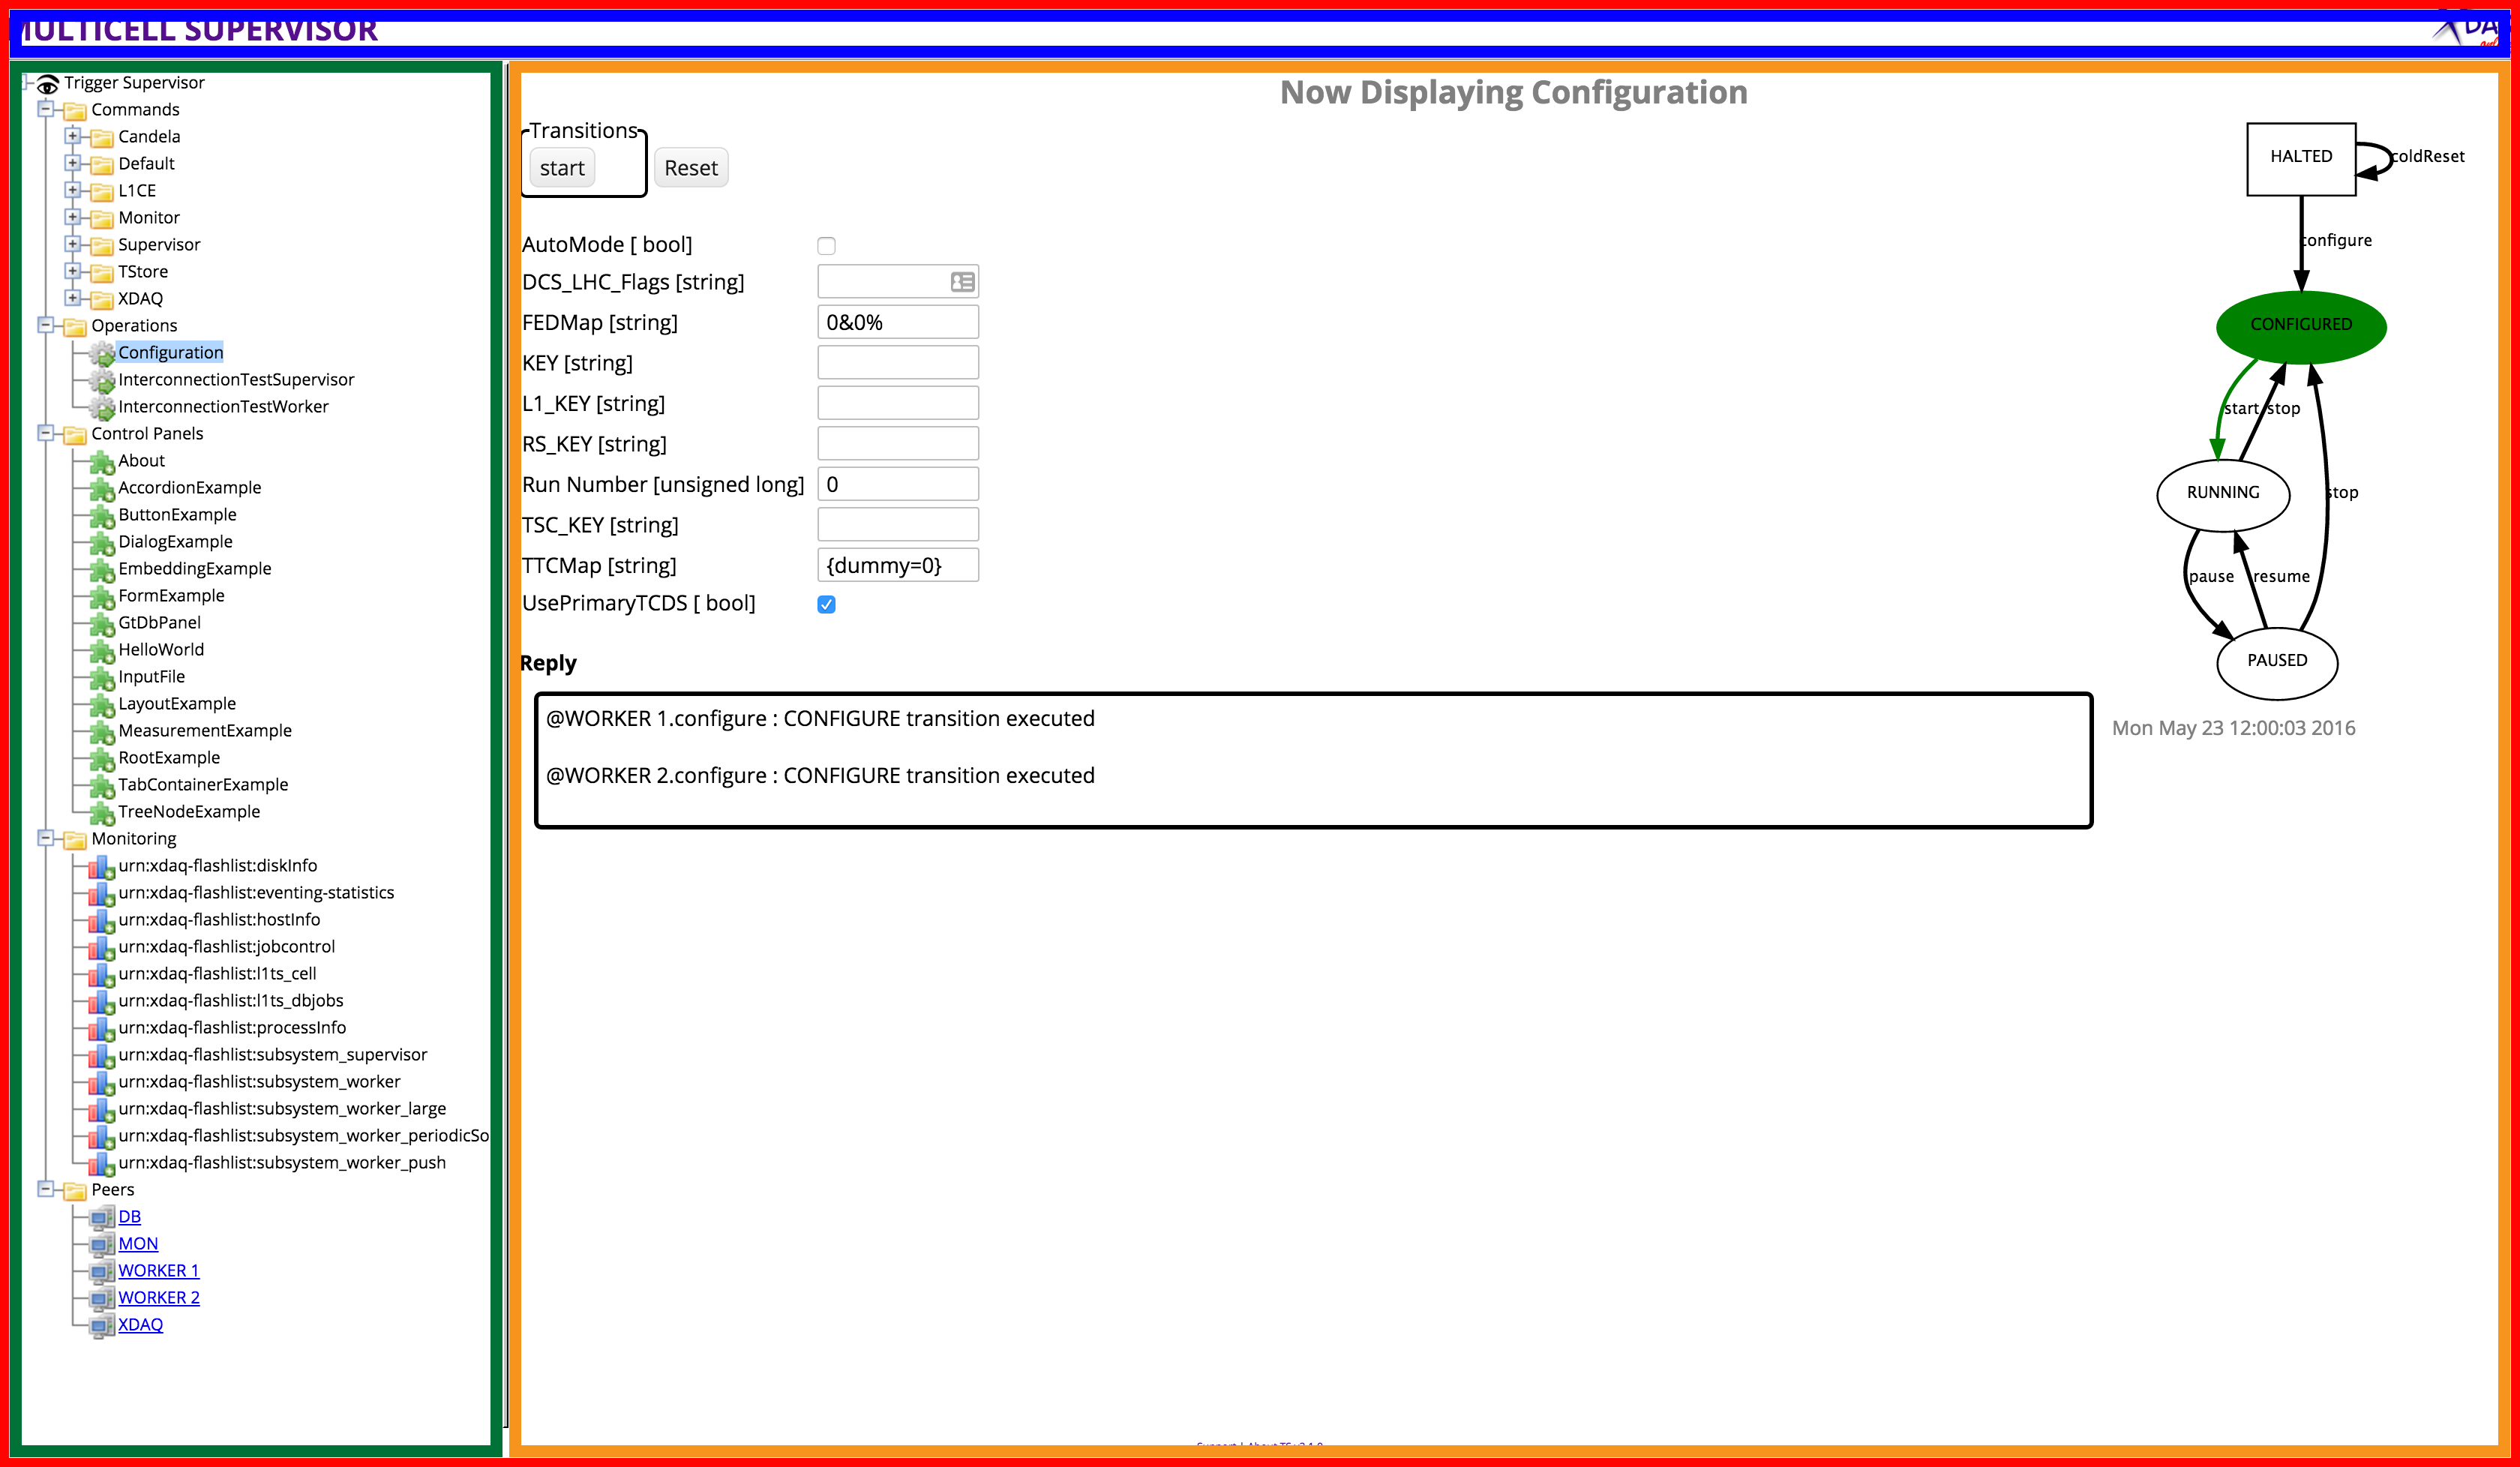
\includegraphics[width=\textwidth]{images/ts2_structure}
  \caption{Screenshot of TS v2.x with main components highlighted.}
  \label{fig:ts2_structure}
\end{figure}

In the new interface, only the `tsgui\_content\_` is kept. This is the Dojo container
where all the panels (legacy & Polymer) are displayed. The menu and top bar
are both handled client-side by a dedicated Polymer element. This is shown in
figure \ref{fig:ts3_structure}.
\begin{figure}
  \centering
  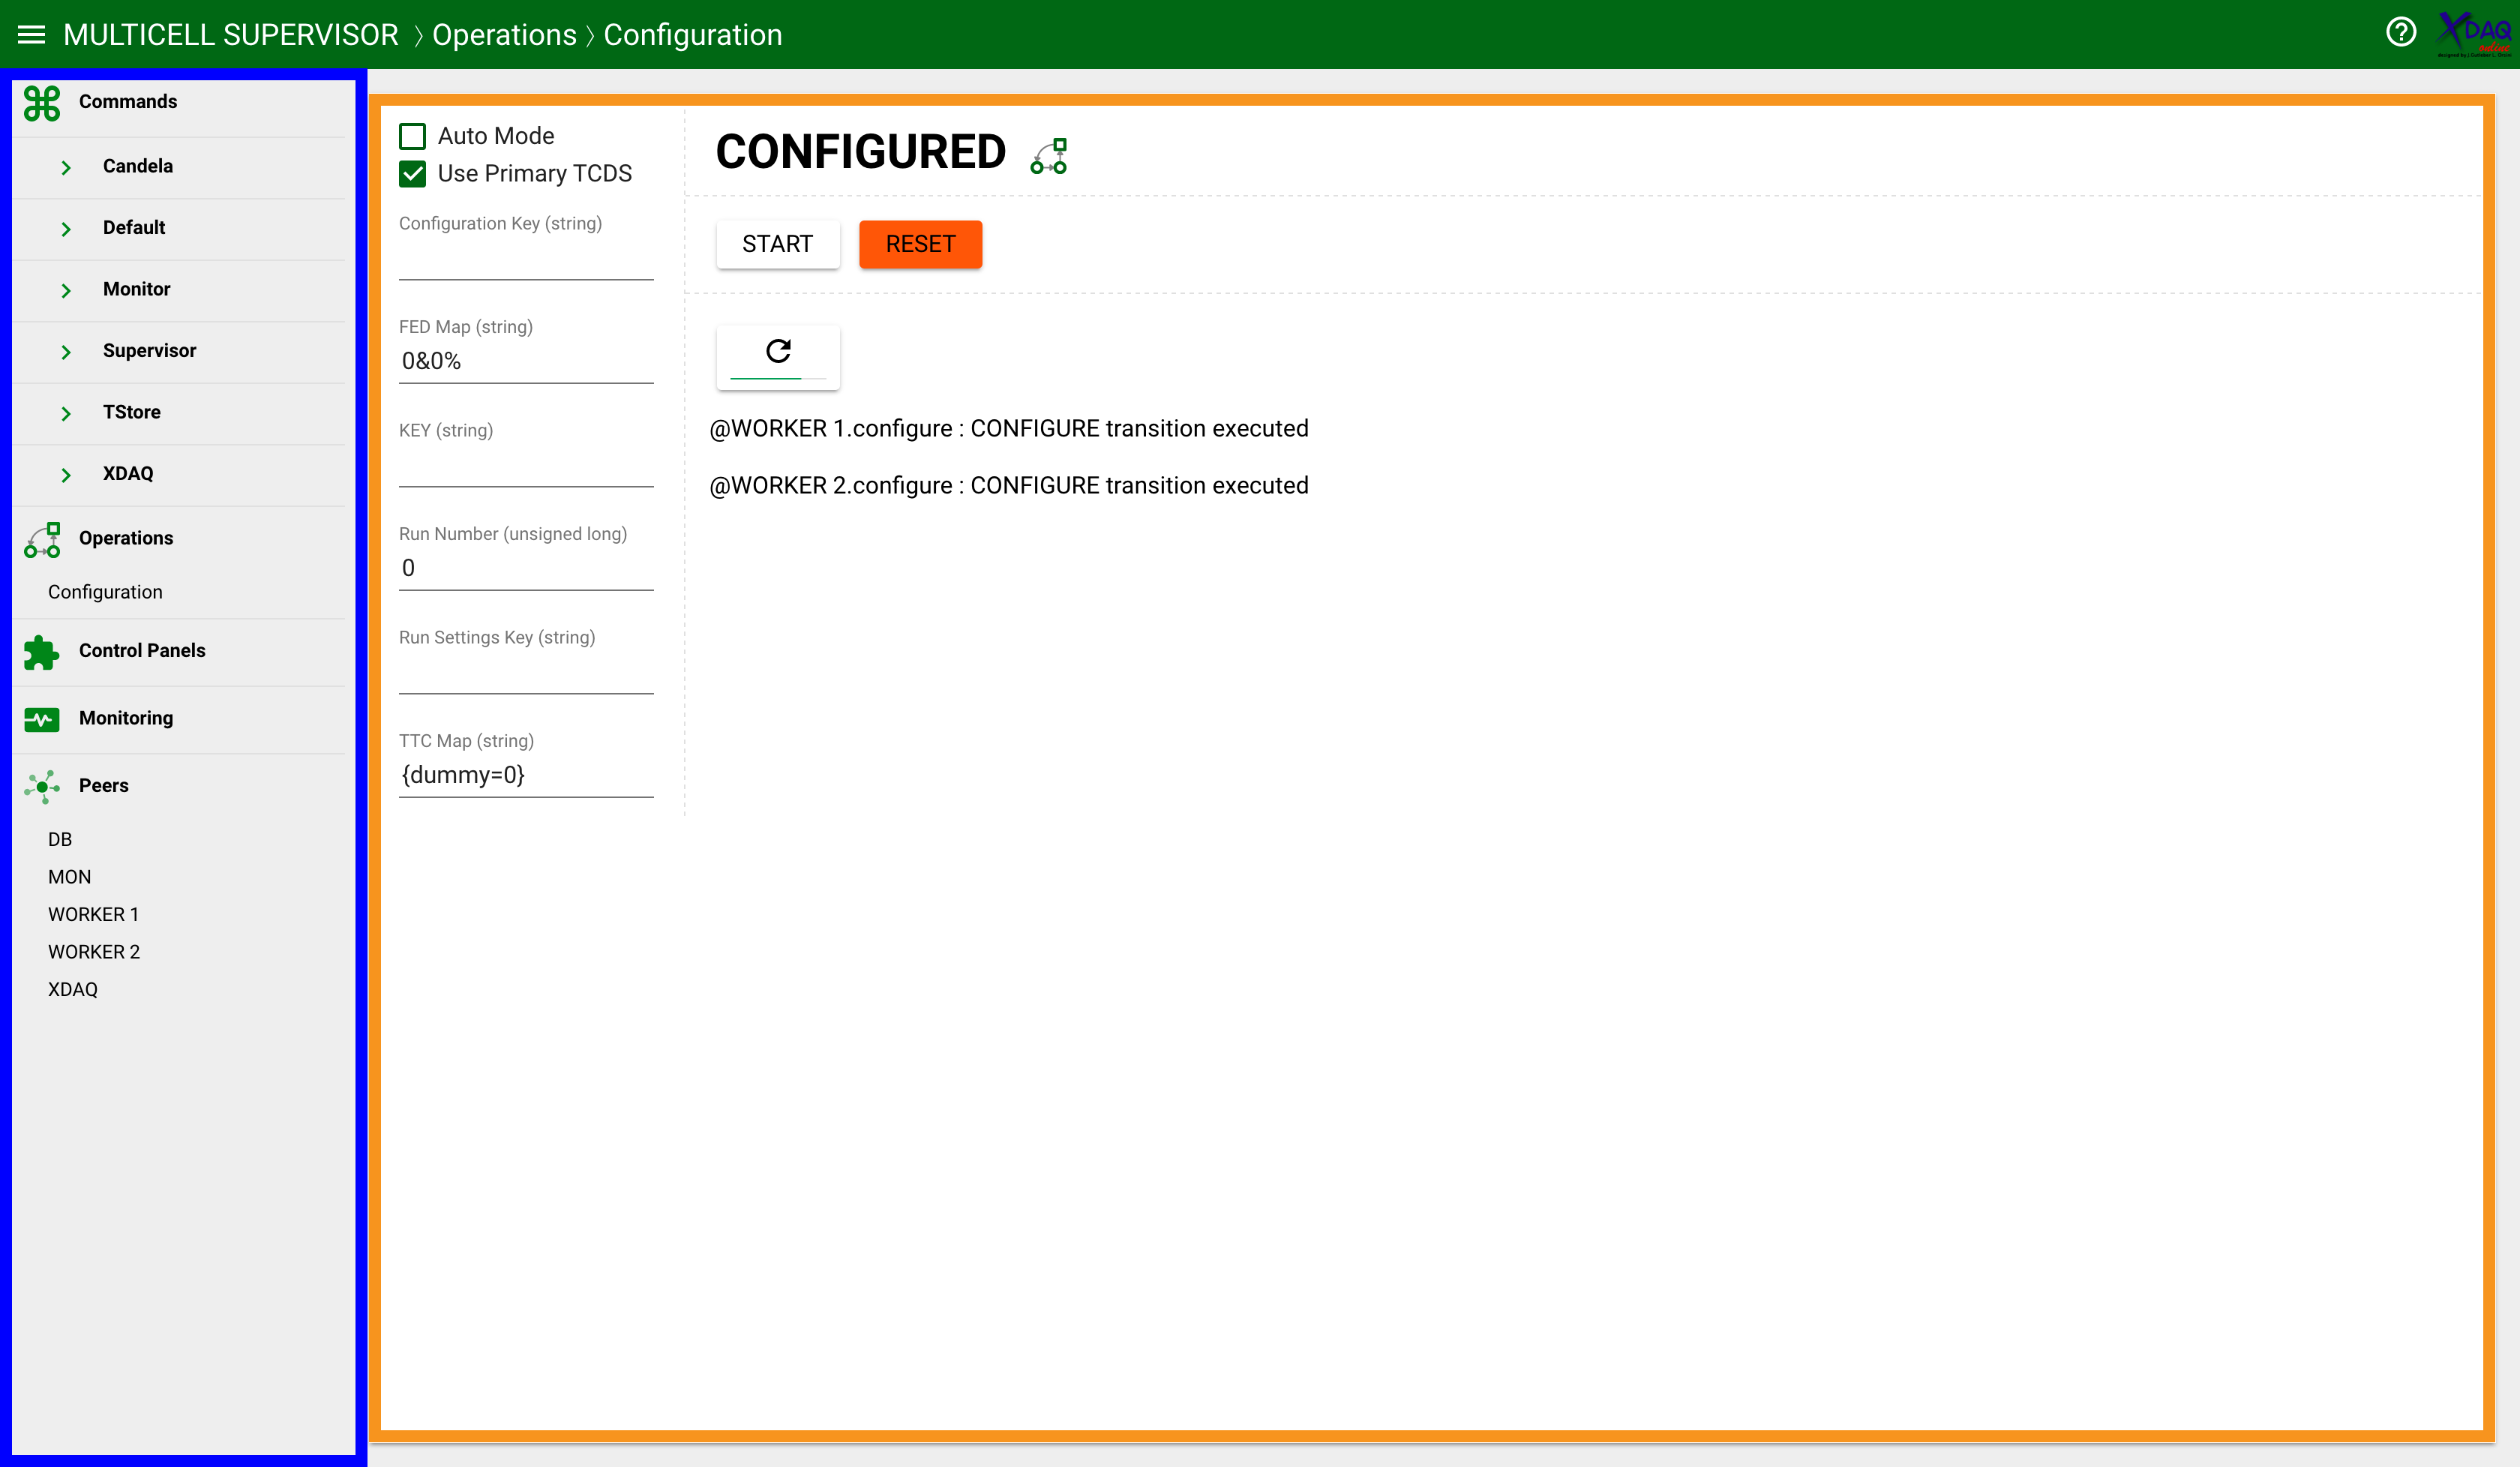
\includegraphics[width=\textwidth]{images/ts3_structure}
  \caption{Screenshot of TS v3.x with main components highlighted.}
  \label{fig:ts3_structure}
\end{figure}

\subsubsection{Session management}
The session is a 48-bit hexadecimal code, and is always encoded in the URL.
This way, if the user tries to interact with the server with an invalid session
token, the server can simply respond with a JavaScript payload redirecting them
to a URL containing a valid session ID.

The URL always looks like this
\begin{lstlisting}
http(s)://host:port/Default?_sesionid_=0x000000000000
\end{lstlisting}
Any state, e.g. the currently loaded panel, is kept server-side in the string
buffers.

\subsection{The new page structure}
The new interface will have the same general structure as the legacy interface,
though updated with the material design look and feel (see chapter \ref{Material Design}),
and some improvements (like a breadcrumb trail).

\subsection{Emulation of the legacy structure in the new page}
The new main page will keep the `tsgui\_content\_` Dojo ContentPane. This way
legacy Dojo panels can still be served, and since the ContentPane is just a plain
`div` tag when not using Dojo it won't inhibit any new code from functioning
properly.

\section{New session management}
The session ID will move out of the URL and will be moved into the response
headers of the server, this header will only be sent if a session change happened.

This approach has a few advantages:
\begin{itemize}
\item The session can now no longer be accidentally shared between users, since
it is no longer contained in the URL.
\item A session renewal does not require a full page reload. The panel will need
to be reset, as the user received a new session, but this will now be much faster
as it doesn't require a full reload.
\item In the old session system the user was navigated to the default page on a
session renewal, and did not preserve the user's navigation through the cell
interface like the new session system does.
In the new system the interface detects the presence of a new session id in any
response of the server, and executes appropriate code to handle a session renewal.
\end{itemize}

\subsection{Material Design}
\label{Material Design}
Material Design (previously called Quantum Paper) is a design language developed
by Google\cite{materialdesign_launch}, released in 2014. It aims to return to the design principles used
in printing, and extend it with things that are normally not possible in real
printing (e.g. motion, responsive layouts, \ldots).

At the center of material design is paper, every component of the design spec
treats a user interface element (e.g. containers, buttons, dropdowns, \ldots) as
a it was being cut out and pasted together with paper.
The reason for this is that it is easier for a user to think with physical objects,

Google uses it to bring back consistency throughout its product line and across
all types of devices. Material design is deployed on watches, phones, tablets,
laptops, and televisions.
Android Marshmallow (v6.x) has fully migrated to material design, and the vast
majority of apps in the Google Play store have adopted it.

The full Material Design spec can be found on the Google design webpage\cite{materialdesign}.

\section{Handling large input}
The legacy (i.e. Dojo) panels sent data back to the server using URL encoding
(more info in chapter \ref{Large input problem}).

The legacy panels can't be adjusted without risking unforeseen consequences.
The new (i.e. Polymer) panels however will all send data back to the server
properly, using HTTP POST requests that contain any parameters in the POST body.

This is the way the HTTP specification designed to send data back to a server,
and thus it solves the problems encountered with sending data with the
legacy code. With the new approach it is now theoretically possible to send 
multi-gigabyte sized data.

\section{Additions to the page builder classes}
The C++ classes in the legacy system each represent an HTML element.
This is manageable because in the set of elements in the legacy system is fixed.
% In the legacy system the set of elements is fixed.
Since in the new system every interface developer will now have the possibility to extend the set of
elements it would make sense to make a more abstract class to handle these new
set of elements.

The ajax::PolymerElement class was added and is used like follows:
\fvset{frame=single}
\begin{pyglist}[language=cpp,numbers=left,numbersep=5pt,fontsize=\small]
ajax::PolymerElement* myElement = new ajax::PolymerElement("my-element");
myElement->set("some-property", "someValue");
add(myElement);
\end{pyglist}
\fvset{frame=none}

Furthermore, the PlainHtml class has been extended with some shorthand functions
to make it easier to use. This because it is a frequently used class.
instead of doing:
\fvset{frame=single}
\begin{pyglist}[language=cpp,numbers=left,numbersep=5pt,fontsize=\small]
ajax::PlainHtml* br53 = new ajax::PlainHtml?();
br53->getStream() << " <p>some html code<p>";
add(br53);
\end{pyglist}
\fvset{frame=none}
it is now possible to do this:
\fvset{frame=single}
\begin{pyglist}[language=cpp,numbers=left,numbersep=5pt,fontsize=\small]
add(new ajax::PlainHtml(" <p>some html code<p>"));
\end{pyglist}
\fvset{frame=none}
This greatly enhances readability of pages containing a lot of arbitrary html code like `<br>`

The AjaXell code has also been modified to support HTML5 features like boolean
attributes (i.e. attributes with no value).

\section{Upgraded event system}
In the legacy codebase, events are attached to C++ classes declared in a panel.
\fvset{frame=single}
\begin{pyglist}[language=cpp,numbers=left,numbersep=5pt,fontsize=\small]
ajax::Button* button = new ajax::Button();
button->setId("subsystem_btnpanel_button_");
button->setCaption("click me!");
this->setEvent(button,ajax::Eventable::OnClick,result_,this,&ButtonExample::onClick);
add(button);
\end{pyglist}
\fvset{frame=none}

However, this system has been extended to allow an event to be attached to the
panel itself, rather than a class instance defined in the panel code.
\fvset{frame=single}
\begin{pyglist}[language=cpp,numbers=left,numbersep=5pt,fontsize=\small]
setEvent("submit", ajax::Eventable::OnClick, this, &FormExample::submit);
add(new ajax::PolymerElement("form-example"));
\end{pyglist}
\fvset{frame=none}

This is necessary because the server will no longer render every element in the
interface. An element (e.g. a button) can be rendered client-side, so

\section{New JSON library}
The primary job of the server-side code will no longer be interface generation,
but data generation.

In the legacy codebase there has been no easy way to generate XML or
JSON data. The only viable way to construct these were to construct them manually
or to use BOOST Property Trees, which require extensive amounts of code.

The TS will incorporate the JsonCpp library, a lightweight C++ library that
makes the generation and parson of JSON very easy.

More information about this can be found in chapter \ref{JsonCpp}.

\section{Memory-leak problem}
\label{Memory-leak problem}
An interface panel can be used for extensive amounts of time, this time can be
expressed in days. Therefore any memory leaks are unacceptable.

Unfortunately it is rather easy to create memory leaks in JavaScript.
JavaScript uses a Reference-counting garbage collection system\cite{IBM_MemoryLeaks}.
Such a garbage collector cannot recognize circular references, and JavaScript
closures add another memory leak pattern to watch out for.

\subsection{Memory-leak patterns}
\subsubsection{Circular references}
A circular reference is formed when two or more objects reference each other in
such a way a closed circle can be drawn.
\begin{figure}[H]
  \centering
  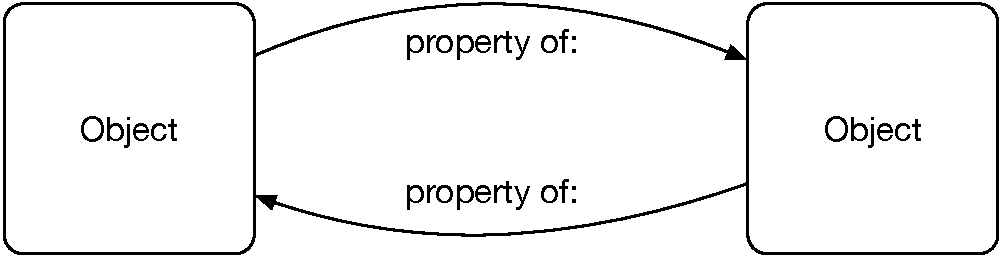
\includegraphics[width=.5\textwidth]{images/circular_reference}
  \caption{A circular reference}
  \label{fig:circular_reference}
\end{figure}

In a reference counting garbage collector like JavaScript these kind of
structures present problems because there is no way the reference count of any
of the object in a circular reference can reach zero, and thus will never be
garbage collected.

The following code will create a circular reference.
\fvset{frame=single}
\begin{pyglist}[language=html,numbers=left,numbersep=5pt,fontsize=\small]
<html>
  <body>
    <div>an HTML element</div>
    <script>
      var div=document.querySelector("div");
      div.someproperty = div;
    </script>
  </body>
</html>
\end{pyglist}
\fvset{frame=none}

This piece of code will however not appear very often. There is not a real use
case where this would appear, and the memory leak is rather obvious.

\subsubsection{JavaScript closures}
A feature of JavaScript is that functions can contain other functions. The inner
function will inherit variables from the parent function.

This inheritance of variables by inner functions is called closure.
This is a code example demonstrating closure:
\fvset{frame=single}
\begin{pyglist}[language=javascript,numbers=left,numbersep=5pt,fontsize=\small]
window.onload = function() {
  var test = 5;
  function innerfn() {
    // will display 5
    alert(test);
  }
  innerfn();
}
\end{pyglist}
\fvset{frame=none}

Closures are the cause of most memory leaks in JavaScript.
Consider the following use case:

An element is created, and a callback is attached to it to react to the click event.
\fvset{frame=single}
\begin{pyglist}[language=javascript,numbers=left,numbersep=5pt,fontsize=\small]
var newelement = document.createElement('p');
newelement.textContent = 'click me';
newelement.onclick = function() {
  alert("you clicked me");
}
document.body.appendChild(newelement);
\end{pyglist}
\fvset{frame=none}
This simple code example contains a memory leak. the function attached to the
onclick event inherits the `newelement` variable, and thus has created a
circular reference.

\subsubsection{Avoiding memory leaks}
Some simple patterns exist to avoid circular references.

Firstly, in a parent function one can set one of the variables causing a
circular reference to null, thereby breaking the circle.
\fvset{frame=single}
\begin{pyglist}[language=javascript,numbers=left,numbersep=5pt,fontsize=\small]
var newelement = document.createElement('p');
newelement.textContent = 'click me';
newelement.onclick = function() {
  alert("you clicked me");
}
document.body.appendChild(newelement);
newelement = null;
\end{pyglist}
\fvset{frame=none}

Another approach is to insert another closure
\fvset{frame=single}
\begin{pyglist}[language=javascript,numbers=left,numbersep=5pt,fontsize=\small]
var inner2 = function() {
  alert("you clicked me");
}
(function inner() {
  var newelement = document.createElement('p');
  newelement.textContent = 'click me';
  newelement.onclick = inner2;
  document.body.appendChild(newelement);
})();
\end{pyglist}
\fvset{frame=none}

Lastly, one can avoid closure altogether.
\fvset{frame=single}
\begin{pyglist}[language=javascript,numbers=left,numbersep=5pt,fontsize=\small]
function callbackfn = function() {
  alert("you clicked me");
}
var function makeElement = function() {
  var newelement = document.createElement('p');
  newelement.textContent = 'click me';
  newelement.onclick = callbackfn;
  document.body.appendChild(newelement);
}
makeElement();
\end{pyglist}
\fvset{frame=none}

\subsection{Memory leaks in Dojo}
\label{Memory leaks in Dojo}
Unfortunately, Dojo 0.4 or the implementation used here seems to contain a lot
of circular references. Memory usage goes up linearly with the amount of panels
used in a browser session.

To test this, a panel will be reloaded (by clicking in the menu) every second.
This will be done for a period of ten seconds, following a 10 second idle period
to allow for any garbage collection to trigger.
This cycle will be executed for sixty seconds, and will be followed by a final
sixty second idle period to make sure any garbage collection has occurred.

The results for this test for TS v2.1.0 is displayed in figure \ref{fig:ts2_memory}.
\begin{figure}
  \centering
  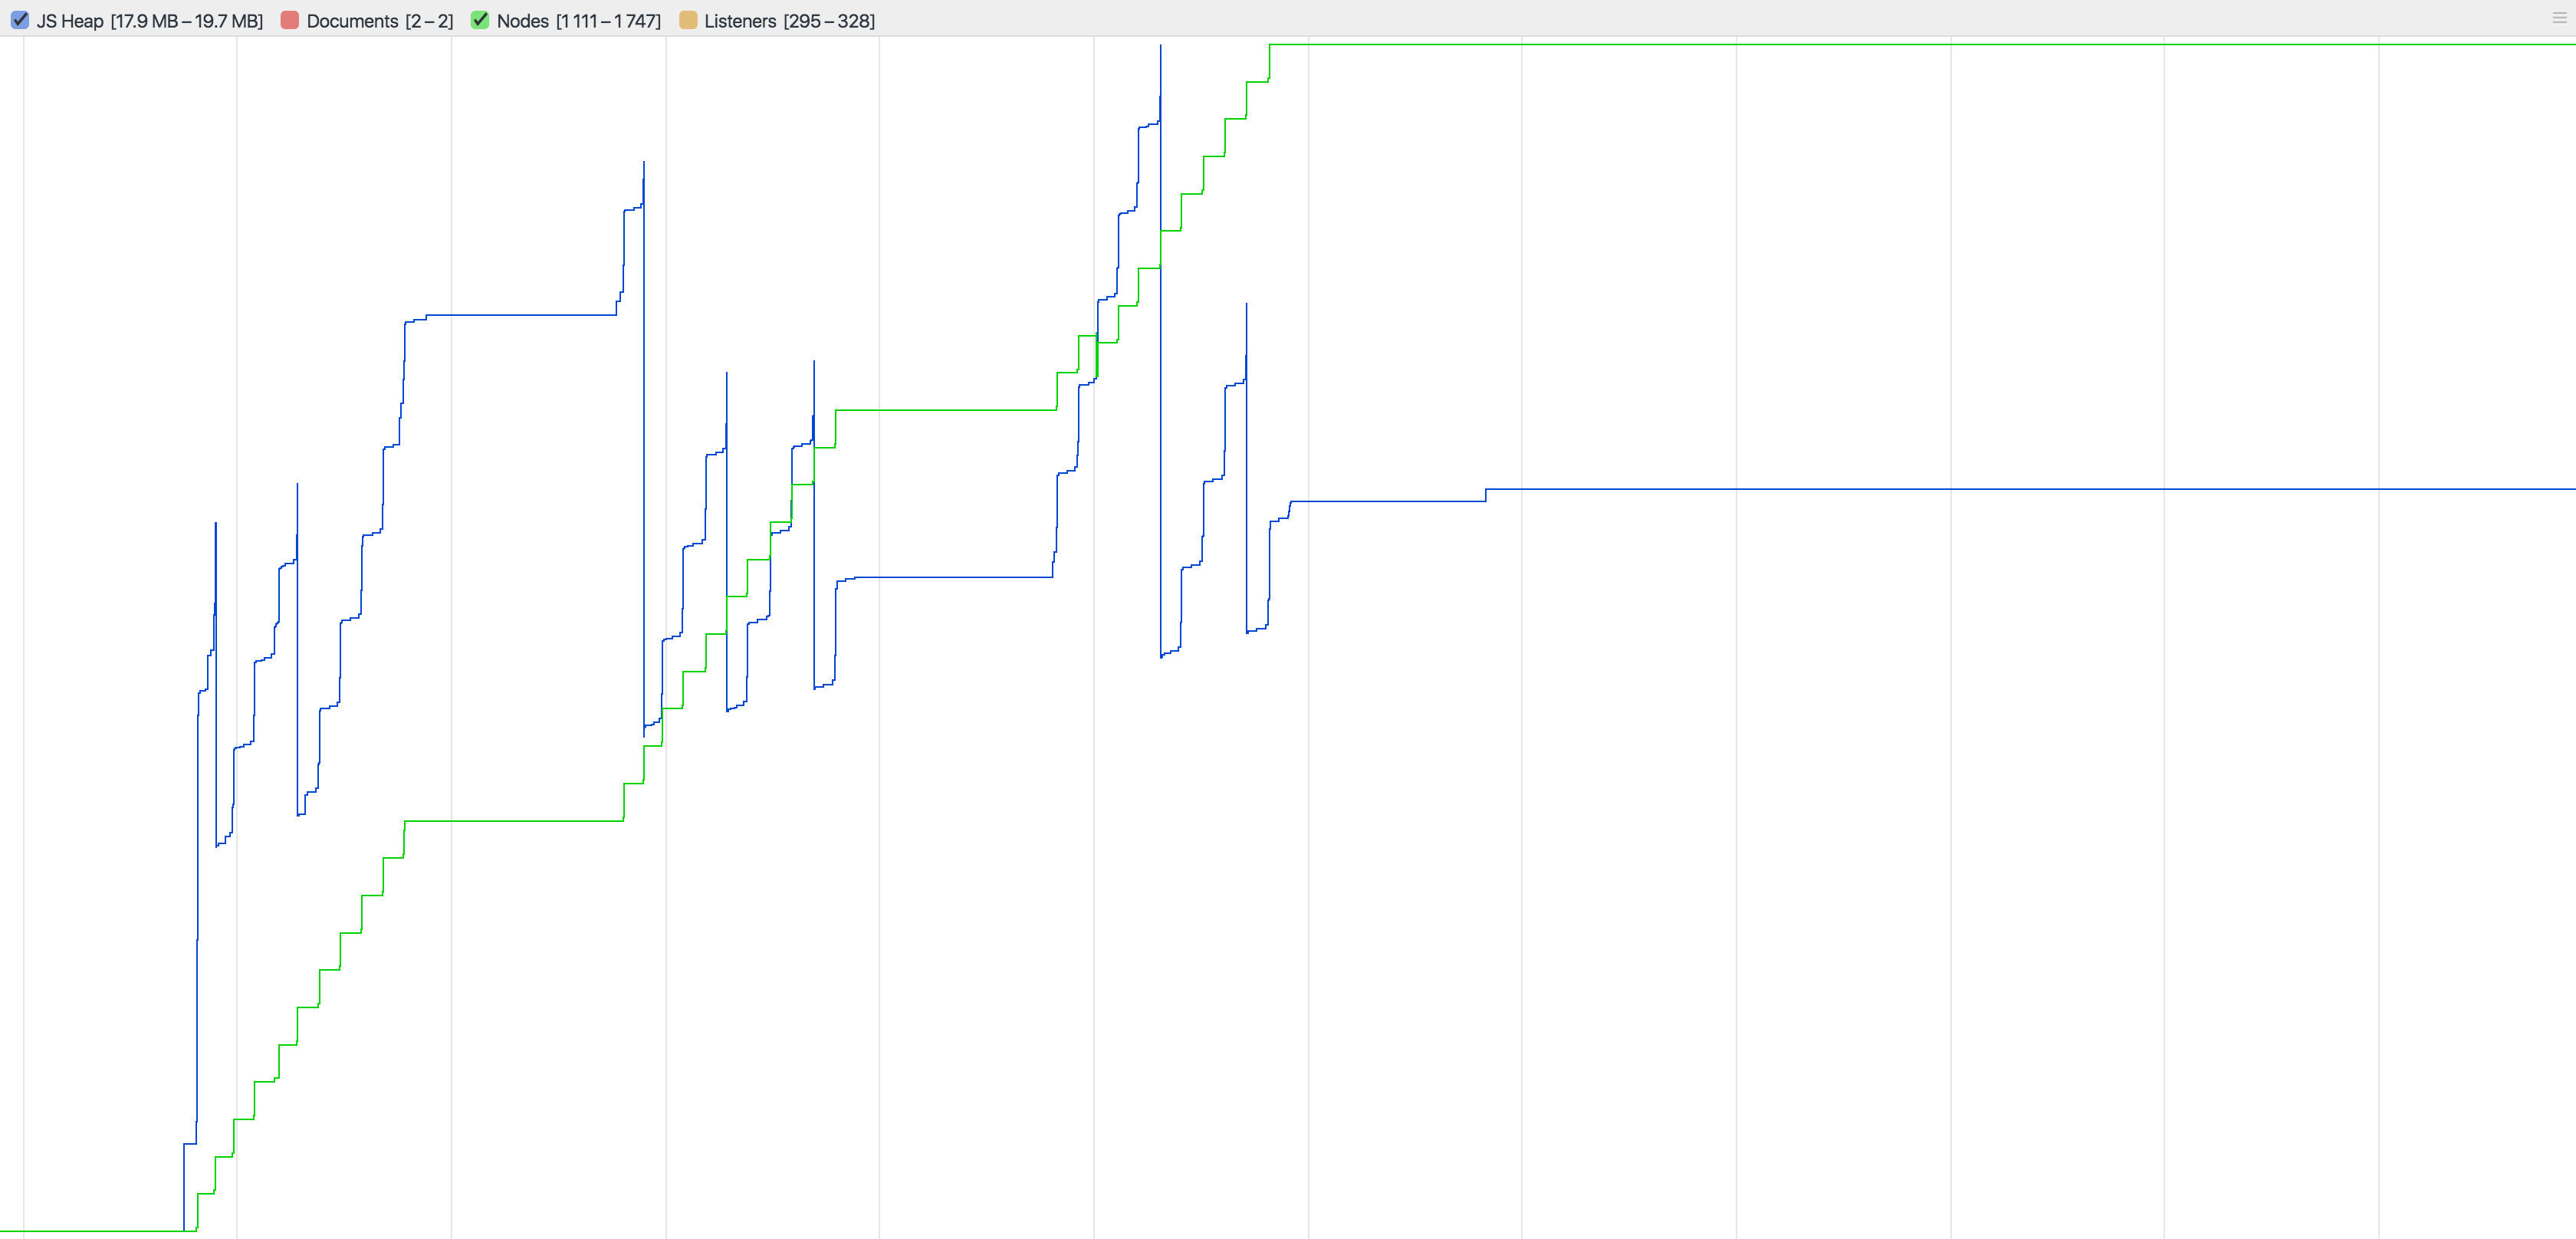
\includegraphics[width=\textwidth]{images/dinosaurs-are-great-120s-run}
  \caption{TS 2.x interface memory usage test}
  \label{fig:ts2_memory}
\end{figure}
Notice that the amount of nodes does not go down. This is because of the circular
references described earlier. The garbage collector will never remove these nodes
from memory, because the reference count of these nodes will never reach zero.

As a result, the memory consumption will grow arbitrarily as panels are used.

In the TS 2.x interface this was not noticed because of the very frequent full
page reloads.
However, with the new graceful session renewal that does not require a page
reload, these memory leaks in dojo panels will pile up until the user manually
refreshes the browser.

Figure \ref{fig:ts3_legacy_memory} shows the result of the same test in the
TS 3.x interface, with the same legacy panel used to test the TS 2.x.
\begin{figure}
  \centering
  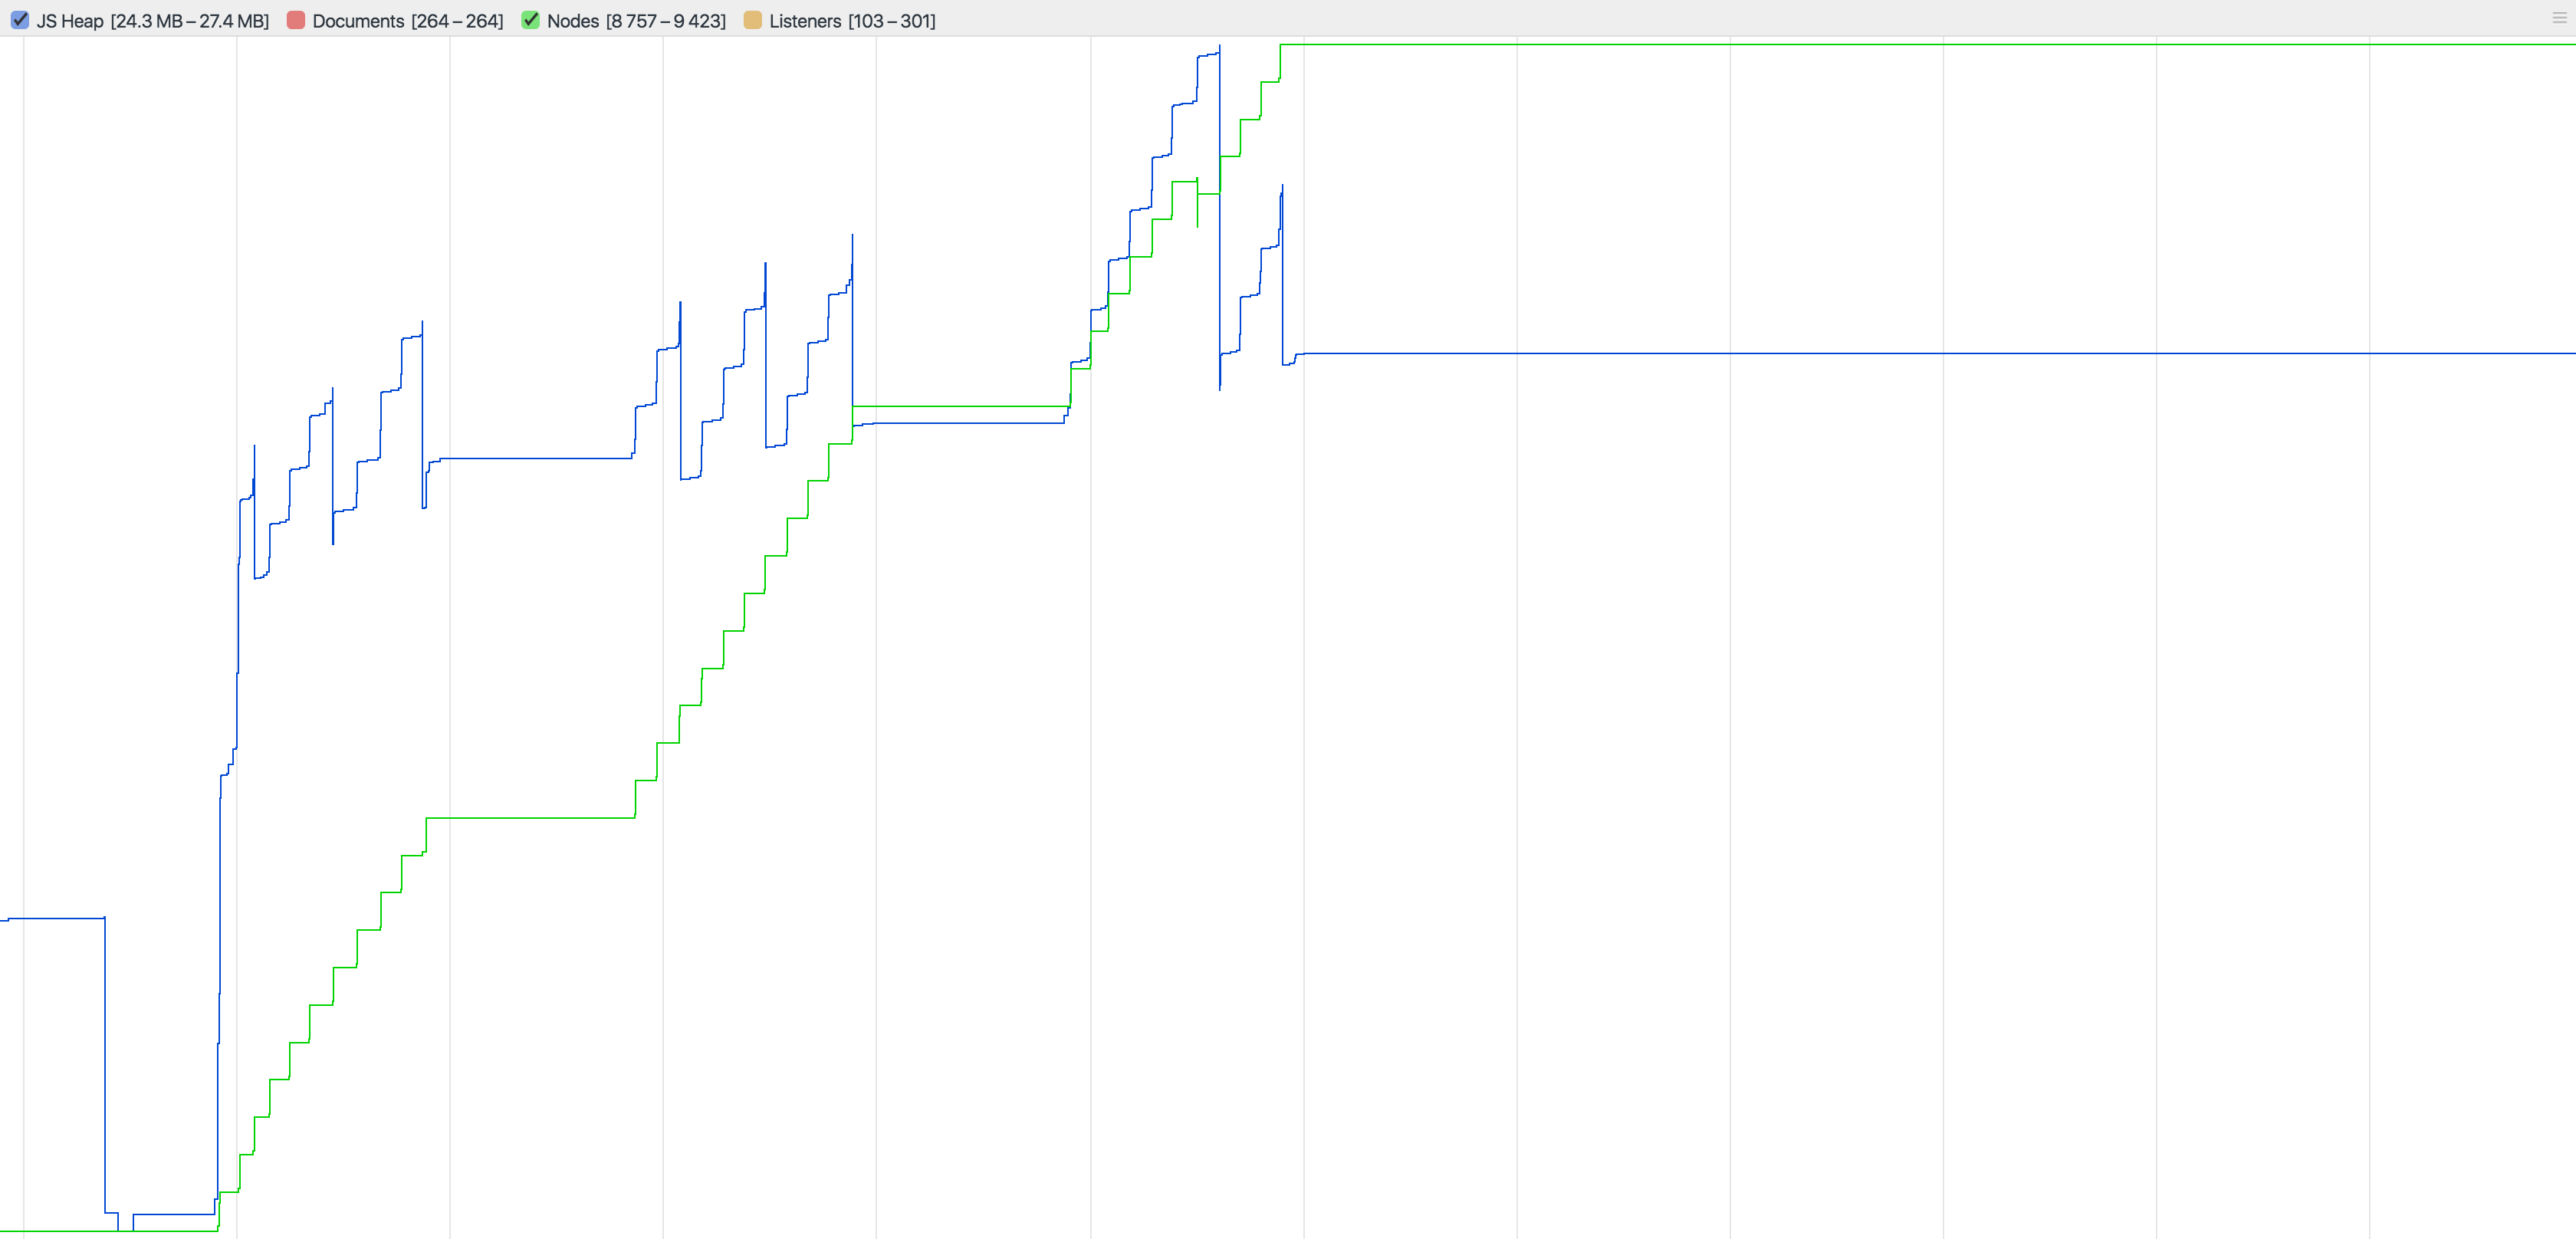
\includegraphics[width=\textwidth]{images/kill-all-roommates-120s-run}
  \caption{TS 3.x interface memory usage test with a legacy panel}
  \label{fig:ts3_legacy_memory}
\end{figure}

Despite the rewritten main interface, the memory leak still occurs with legacy
panels. This is because the cause of the memory leak resides inside the Dojo
library itself.

A solution to this problem is not easily apparent. It would require changes to
the legacy codebase, which is always a risky thing to do.
It is decided that for this reason, any legacy panel that features automatic
refreshes (e.g. the operations panel) has a high priority to be replaced with a
polymer alternative.

\subsection{Memory leaks in Polymer}
\label{Memory leaks in Polymer}

The same test is done again in the TS 3.x interface, but with the panel being
upgraded to a Polymer equivalent. The results are shown in figure \ref{fig:ts3_memory}.

Note that this time, the garbage collector is able to remove unused DOM nodes
from memory, followed by the memory usage returning to its original value
immediately after the test.

\begin{figure}
  \centering
  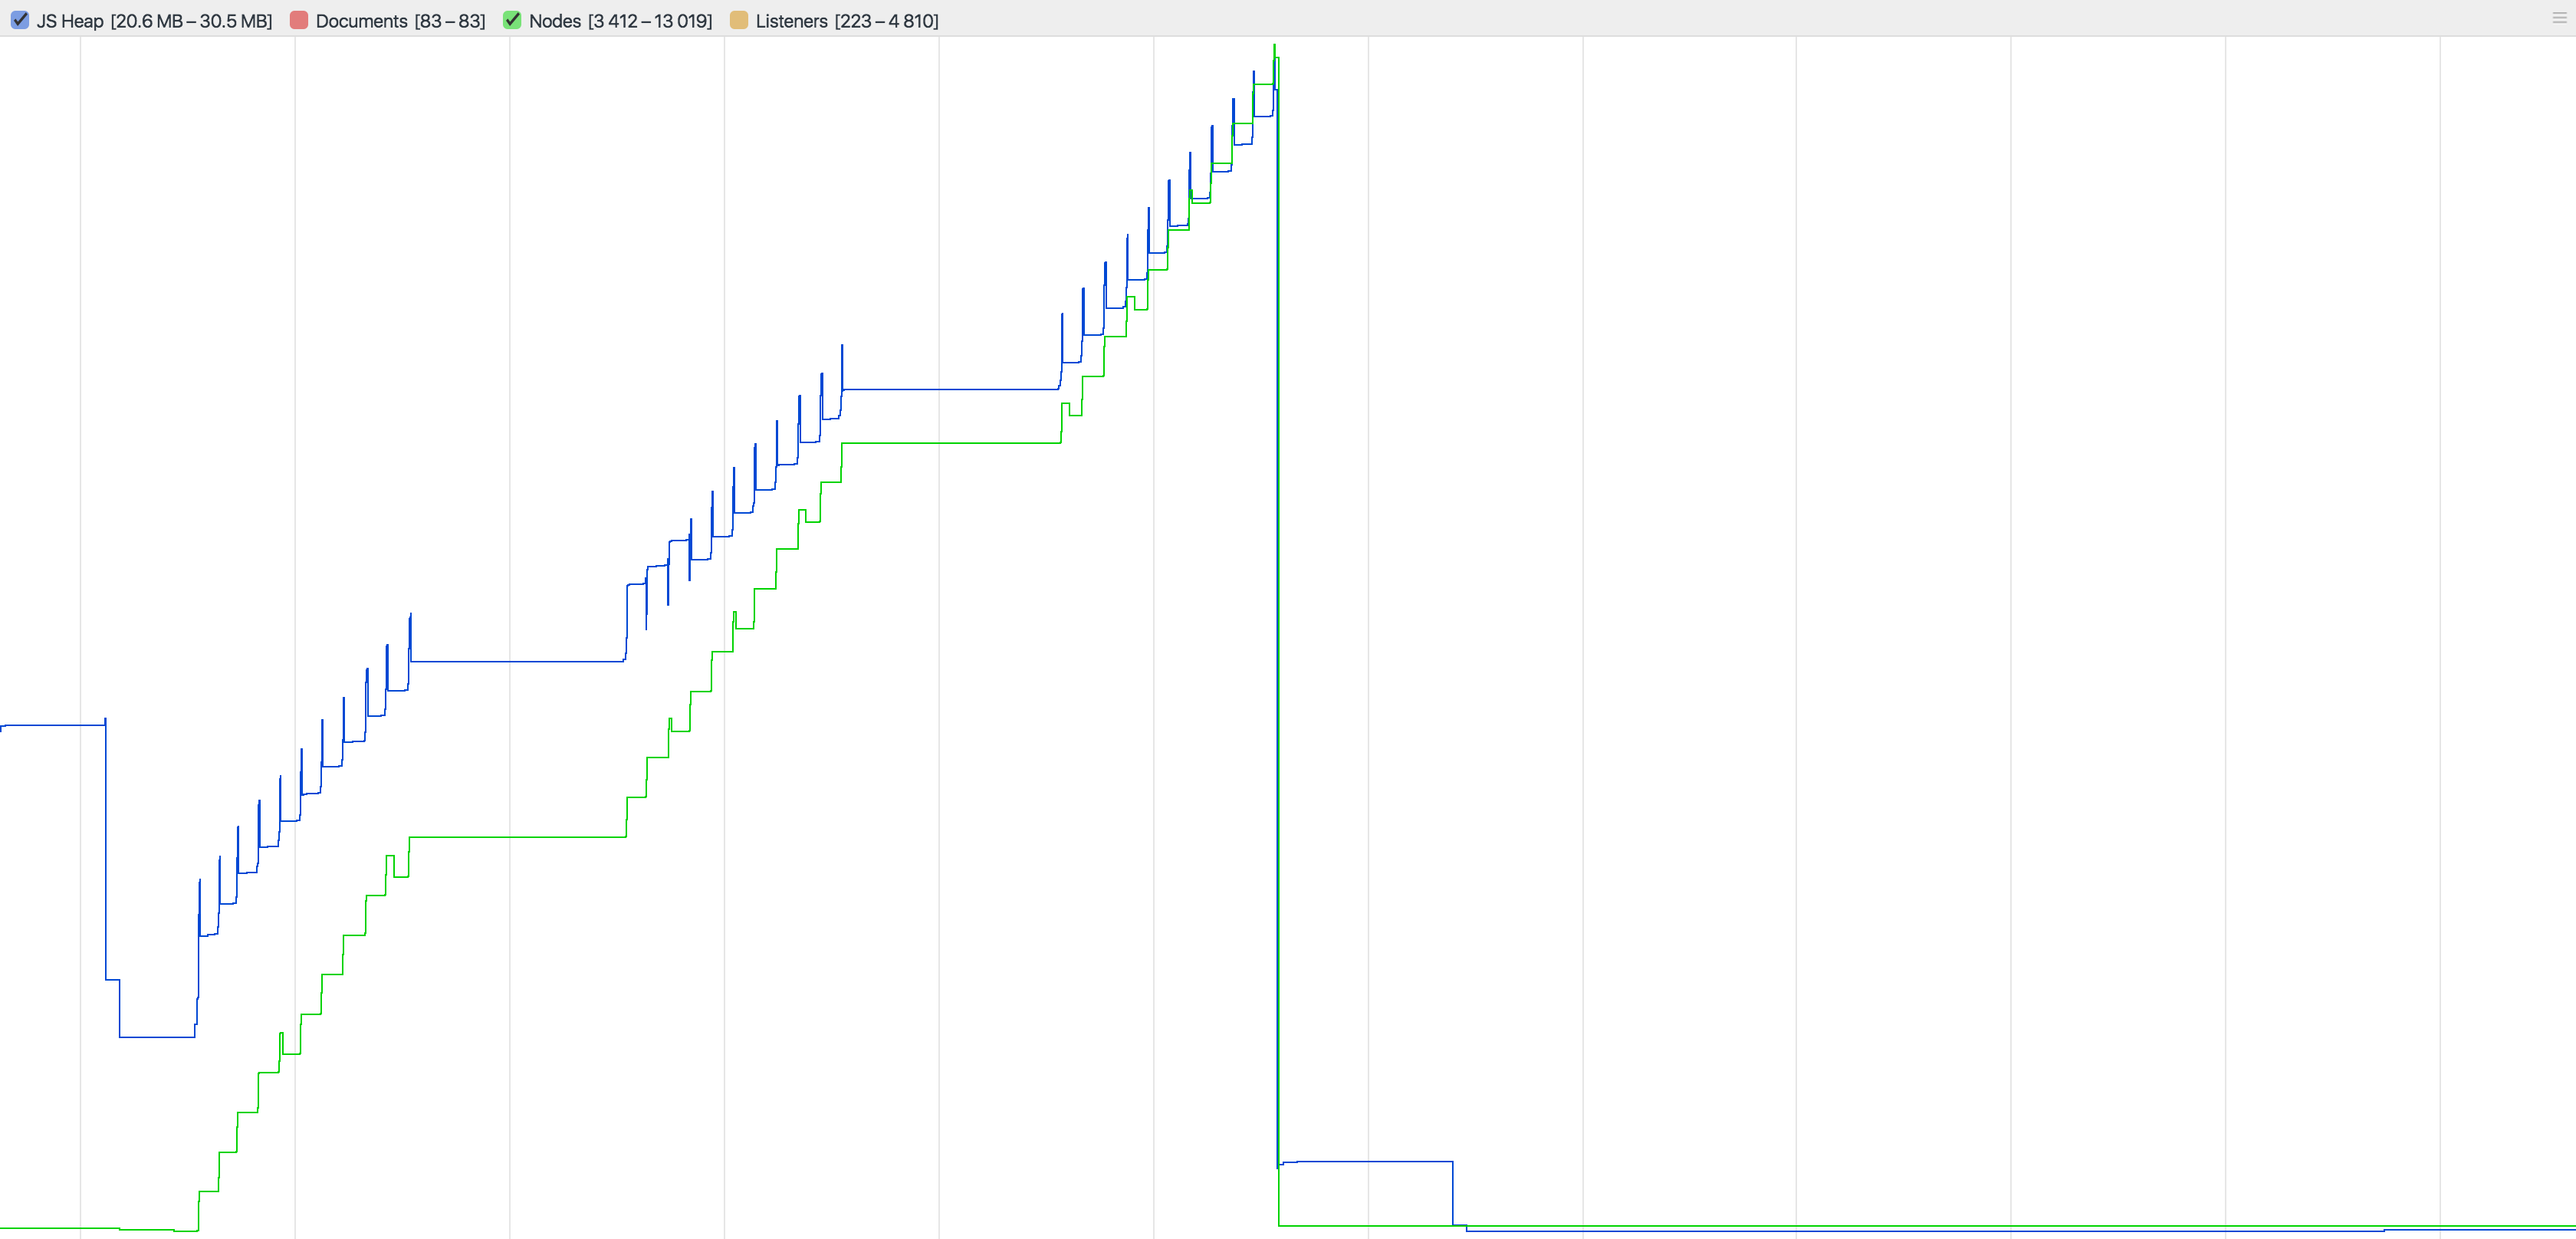
\includegraphics[width=\textwidth]{images/kill-all-humans-120s-run}
  \caption{TS 3.x interface memory usage test with a Polymer panel}
  \label{fig:ts3_memory}
\end{figure}

\chapter{Development process}
Given the size of the TS and the amount of stakeholders in the proposed changes,
it is important to have a decent planning.

The main objectives are productivity, and making sure developers deliver what is needed most
at a particular moment.

It also would be nice to have a sensible feedback system to allow the stakeholders
to have an influence in the evolution of the TS changes, as they will be the
people who are going to use it.

A modified version of the Scrum method has been used as the development process.
The modifications are focused on providing compatibility with the other development
processes in use by other developers.
Also it has been modified to account for the limited amount of people working on
one task.

\section{Scrum}
Scrum is a relatively new way of developing software projects, although it has
also been used to execute projects not related to development (e.g. construction
projects).

It focuses on delivering functional requirements prioritized on the value it adds
to the project as a whole.

It implements a very strict and repetitive development cycle, usually with a
period of 1 or more weeks. This is called a Sprint. During the beginning of a
Sprint, a set of functional requirements are chosen as a goal, and must be
achieved by the end of the Sprint.

An important distinction to make is that the developers themselves drive this
process. There is no separate person who makes the planning and the set of
requirements for a Sprint on their behalf.
This is where Scrum gets efficient, because the developers after all know best
what is most important and feasible to achieve in one full Sprint.

At the end of a Sprint a set of functional requirements must be met. This means
that particular set of functionality in the project must work in a sense that
the end user can use it. This must be proven by a working demo to the
stakeholders of the project, all of them.

This is also a very important part of Scrum. By demanding the functionality
must work to such an extend that it would be useful for deployment means there
is far less opportunity for hidden errors during actual deployment.
The working demos to all of the stakeholders also provide feedback to
developers at early stages, unlike other systems where stakeholders only get to
see the product all the way at the end of the product development and notice the
developers and stakeholders had some different ideas about functionality.

For more info about Scrum can be found in the book written by one of its inventors,
Jeff Sutherland\cite{scrumbook}.

\subsection{Kanban}
Tasks are divided into distinctive and sequential states. Each task must flow
through each state.
A change in the task results in that task being reset to the initial state.

The following states were chosen for a task:
\begin{labeling}{In productionnnn}
\item [\textbf{Backlog}] This is a list of all the tasks that need to be done.
They are not part of a Sprint, but are the list of candidate tasks for a Sprint.\\
\item [\textbf{To do}] Tasks get moved from the backlog to `To do` when they are
selected to be part of the currently starting Sprint. This list represents the
set of tasks that need to be competed (i.e. be in the `Done` state) by the end of
the Sprint.\\
\item [\textbf{In progress}] When someone is working on a particular task, it is
moved from `To do` to `In progress`.\\
\item [\textbf{In review}] A task get put into `In review` when it is considered
ready for use. At this stage another developer double checks the new functionality.
The main objective is detecting missing features or a misunderstood implementation of it.\\
\item [\textbf{Testing}] At this point the code of a task is pushed to the SVN
repository. The relevant code is then recompiled and tested by a few experts (i.e.
people who will be using this panel).\\
\item [\textbf{Done}] After testing is complete, a task is considered `Done` and
awaits a new software release to be put in `In production`.\\
\item [\textbf{In production}] Once a new release of the TS is pushed to production
systems, the appropriate tasks are moved to `In production`. A task in this state
can be deleted from the point it can be reasonably assumed the relevant features
are stable.\\
\end{labeling}

Trello (\url{https://trello.com/}) has been the tool of choice to implement this
Kanban board (see figure \ref{fig:Kanban}).

\begin{figure}
  \centering
  \includegraphics[width=\textwidth]{images/Kanban}
  \caption{Screenshot of the Trello Kanban board used during development}
  \label{fig:Kanban}
\end{figure}

\subsection{Workflow}
The Scrum process has been modified to account for the tiny number of developers.

Every week a list of functional requirements is made, preferably this does not
encompass any technical goals and thus only contains goals towards end-user
functionality. These are formed into tasks and get put into the backlog.

This list is then sorted according to urgency and importance (urgency takes
precedence over importance).
After sorting, the backlog items are considered to be put into `To do` status up
until a point the Sprint contains enough tasks.

After the tasks have been done, they are in the `In review` stage. Where they will
be either reviewed internally or reviewed during the weekly or monthly meetings
depending on the importance of the feature.

\section{Version Control}
Apache Subversion (SVN) is used to implement version control with the online
software source code.

It is accompanied by a web based ticketing system based on Trac (\url{https://trac.edgewall.org/}).

The repository structure follows all common best practices. The `trunk` folder
contains strictly working and tested code and is used to perform the nightly builds.
It has a `branches` folder containing any pending bug fixes or added features.
Branches follow the `username\_foldername\_ticket\#` naming convention.
The repository also has a `tags` folder, containing working copies of the source
code that are associated with a specific version (e.g. 2.0.1).

The versioning system uses three numbers to signify major, minor, and patch changes,
respectively.

This repository can be found at \url{https://svnweb.cern.ch/trac/cactus}

\chapter{Polymer}
Polymer allows a developer to declare new web Components. This is used to generate
the custom web interfaces.

This chapter describes how Polymer is used and what developers can do with it.

\section{From C++ to Polymer}
As stated in chapter \ref{Separation of Concerns}, C++ should only be used for
data generation.

However, to keep compatibility with legacy code, the string buffer
system is still used. Therefore the interface must be initiated like so:
(this example is taken from the Flexbox layout example in the Subsystem Supervisor)
\fvset{frame=single}
\begin{pyglist}[language=cpp,numbers=left,numbersep=5pt,fontsize=\small]
#include "subsystem/supervisor/panels/FlexboxLayout.h"
#include "ajax/PolymerElement.h"

using namespace subsystempanels;
FlexboxLayout::FlexboxLayout( tsframework::CellAbstractContext* context,
                              log4cplus::Logger& logger)
:tsframework::CellPanel(context,logger) {
  logger_ = log4cplus::Logger::getInstance(logger.getName() +".FlexboxLayout");
}

void FlexboxLayout::layout(cgicc::Cgicc& cgi) {
  remove();
  add(new ajax::PolymerElement("flexbox-layout"));
}
\end{pyglist}
\fvset{frame=none}

There is still a tiny piece of C++ code that renders the initial HTML
code, at line 13.
It merely specifies the name of the Web Component that renders the panel interface
for the Flexbox layout example panel.

\section{From Polymer to C++}
\label{From Polymer to C++}
The previous example did not contain any data generation.

In order to add support for a callback, it must be registered like so:
(this example is taken from the Form example panel in the Subsystem Supervisor)
\fvset{frame=single}
\begin{pyglist}[language=cpp,numbers=left,numbersep=5pt,fontsize=\small]
  #include "subsystem/supervisor/panels/FormExample.h"
  #include "ajax/PolymerElement.h"
  #include "ajax/toolbox.h"
  #include "json/json.h"

  using namespace subsystempanels;
  FormExample::FormExample( tsframework::CellAbstractContext* context,
                            log4cplus::Logger& logger)
  :tsframework::CellPanel(context,logger) {
    logger_ = log4cplus::Logger::getInstance(logger.getName() +".FormExample");
  }
  FormExample::~FormExample() {
    remove();
  }

  void FormExample::layout(cgicc::Cgicc& cgi) {
    remove();
    setEvent("submit", ajax::Eventable::OnClick, this, &FormExample::submit);
    add(new ajax::PolymerElement("form-example"));
  }

  void FormExample::submit(cgicc::Cgicc& cgi,std::ostream& out) {
    std::map<std::string,std::string> values(
      ajax::toolbox::getSubmittedValues(cgi)
    );

    Json::Value root(Json::arrayValue);

    for(
      std::map<std::string,std::string>::iterator i(values.begin());
      i != values.end(); ++i
    ) {
      Json::Value someresult;
      someresult["name"] = i->first;
      someresult["value"] = i->second;
      root.append(someresult);
    }

    out << root;
  }
\end{pyglist}
\fvset{frame=none}

Now a callback `submit` is registered, which will execute the FormExample::submit
function and return whatever output it generated.

These callbacks can be implemented in Polymer using the `ts-ajax` or the `auto-update`
element in the `common-elements` package.

\fvset{frame=single}
\begin{pyglist}[language=html,numbers=left,numbersep=5pt,fontsize=\small]
<dom-module id="form-example" >
  <template>

    <ts-ajax id="ajax"
             callback="submit"
             data="{{response}}"
             parameters='["sometextinput"]'
             sometextinput={{text1}}></ts-ajax>
    <paper-input label="some text input"
                 value="{{text1}}" ></paper-input>

    <paper-fab icon="send" title="send" on-click="submit" ></paper-fab>

    <h1>server response:</h1>

    <template is="dom-repeat" items="[[response]]" as="item" >
      <p>[[item.name]] = [[item.value]]</p>
    </template>

  </template>
  <script>
    Polymer({
        is: 'form-example',

        properties: {
          response: {
            type: String,
            value: undefined
          }
        },

        submit: function() {
          this.$.ajax.generateRequest();
        }
    });
  </script>
</dom-module>
\end{pyglist}
\fvset{frame=none}

\section{Polymer features}
Polymer is bundled with a lot of useful functionality out of the box.
The most used ones in this project are described here.

A more detailed explanation can be found at the Polymer docs\cite{polymerdocs}
\subsection{Properties}
Polymer elements can contain custom properties defined by the developer.
A property can be an object, a date, a string, a number, an array, a boolean, or a function.
They can be configured to be read-only, to spawn events and/or execute functions
when their value changes.

Properties are useful to display to, or get data from, the user.
\subsection{Data binding}
Data binding is used to connect properties between web components or to bind a
property to a control like an input box or a button value.

It is also useful to automatically fetch data from the server and put it in the
interface without much effort. An example of this can be found in chapter \ref{From Polymer to C++}.
\subsection{Lifecycle callbacks}
A web component can react to lifecycle events. This allows a developer to write
code to be executed when a new instance of the web component is created, or
when it is placed inside the DOM tree, or removed from it.

A useful example is the `auto-update` element, which declares an interval on the
`attached` event, and removes it on the `detached` event.
\subsection{Styling}
AjaXell provides developers with a theme. This is provided in the form of a
web component called `reset-css`. It makes other web components conform to the
AjaXell them (e.g. button size, fonts, colors, \ldots).

Also Polymer gives developers the possibility to use CSS functionality that is
not yet implemented in all browsers, but which are very useful for web components.

One of them is CSS variables and mixins, which allows a developer to define variables in CSS.
Notable is that these variables are inherited just like normal properties.
This is how the AjaXell theme file defines its theme colors.
\fvset{frame=single}
\begin{pyglist}[language=css,numbers=left,numbersep=5pt,fontsize=\small]
:root {
  --primary-color: #00671a;
  --warning-color: yellow;
  --text-color: black;
  --fancy-gradient: {
    background: linear-gradient(to bottom,
                                #1e5799 0%,
                                #2989d8 50%,
                                #207cca 51%,
                                #7db9e8 100%);
  }
}
paper-button {
  color:var(--text-color);
  --paper-button-ink-color:var(--primary-color);
}
paper-button.warning {
  --paper-button-ink-color:var(--warning-color);
}
div[fancy] {
  @apply(--fancy-gradient);
}
\end{pyglist}
\fvset{frame=none}

A Polymer element can include this theme by including it in its template.
\fvset{frame=single}
\begin{pyglist}[language=html,numbers=left,numbersep=5pt,fontsize=\small]
<link rel="import" href="/ts/common-elements/reset-css/reset-css.html" >
<dom-module id="my-element" >
  <template>
    <style include="reset-css" ></style>
    <paper-button>I am themed!</paper-button>
  </template>
  <script>Polymer({is: 'my-element'});</script>
</dom-module>
\end{pyglist}
\fvset{frame=none}

\subsection{Events}
An element can define define events. It can also react to any event spawned by
elements in its template using the following syntax:

\fvset{frame=single}
\begin{pyglist}[language=html,numbers=left,numbersep=5pt,fontsize=\small]
<dom-module id="my-element" >
  <template>
    <!-- paper-button fires 'click' event -->
    <paper-button on-click="clicked" >Click me!</paper-button>
  </template>
  <script>
    Polymer({
      is: 'my-element',
      clicked: function(e, detail) {
        this.fire('kick', {kicked: true});
      }
    });
  </script>
</dom-module>
<my-element></my-element>
<script>
  document.querySelector('my-element').addEventListener('kick', function (e) {
    if (e.detail.kicked) {
      console.log("kick event fired");
    };
  });
</script>
\end{pyglist}
\fvset{frame=none}

\subsection{Behaviors}
Behaviors in Polymer is a way to share JavaScript code among multiple elements.
A useful example of this is the `throws-toast` behavior in common-elements,
which allows an element to show notifications to the user.

The throws-toast.html behavior definition looks like this:
\fvset{frame=single}
\begin{pyglist}[language=html,numbers=left,numbersep=5pt,fontsize=\small]
<script>
throwsToast = {
  /**
   * Throw a message to the central toaster.
   * The `Toast` object accepts the following properties:<br>
   * type (String): Can be 'info', 'warning', or 'error'.<br>
   * message (String | HTMLElement): The actual message to show.<br>
   * options (Array of Strings) (optional): This will force the user
   * to stop what they're doing and choose one of the supplied
   * options. The chosen option is returned.
   *
   * @param {Toast} toast Can be 'info', 'warning', or 'error'.
   * @param {function} callback The function to invoke when one of
   * the options has been clicked.
   * Takes the option string as argument.
   * @return {Void | String}
   */
  throwToast: function(toast) {
    if (typeof toaster === "undefined") {
      console.error(this, "toaster is undefined");
    } else {
      toaster.throwToast(toast, this);
    }
  }
};
</script>
\end{pyglist}
\fvset{frame=none}

An element can implement it like this:
\fvset{frame=single}
\begin{pyglist}[language=html,numbers=left,numbersep=5pt,fontsize=\small]
<link rel="import" href="/ts/ajaxell/html/elements/ag-toaster/throws-toast.html" >
<dom-module id="notifications-demo" >
  <template>
    <paper-button warning on-click="showWarning" >show warning</paper-button>
  </template>
  <script>
    Polymer({
      is: 'notifications-demo',
      behaviors: [throwsToast],
      showWarning: function showWarning() {
        this.throwToast({
            'type': 'warning',
            'message': 'this is a warning at t=' + new Date().getTime(),
            'callback': function callback(response) {
                console.log("callback successfull: ", response);
            }
        });
      },
    });
  </script>
</dom-module>
\end{pyglist}
\fvset{frame=none}

\chapter{The renewed panel SDK}
The new front-end and back-end codebase provide an interface developer with a
whole new set of tools.

\section{Packages available to panel developers}
The set of pre-made tools available to developers has vastly expanded.

Not only does this mean a more rich set of tools are developed internally,
developers can now also find and include tools they find on the web.

This will provide a way to get the framework capabilities to evolve as time
goes on.

\subsection{Bower Components}
All libraries, web components, sources, \ldots that are not developed in-house
are housed in the bower-components package.
The name is derived from the package manager used to pull in these resources,
called `bower` (\url{http://bower.io/}).

The bower-components package contains a `bower.js` file that specifies the
dependencies to be pulled from the web.
Then the dependencies are compressed into a tarball. This is done to make sure
the package versions do not change unintentional, and new package versions can
be tested in a controlled manner.

Currently, the following elements are included in bower-components:

\begin{labeling}{vaadin-core-elementssss}
\item [\textbf{Polymer}] (\url{https://www.polymer-project.org/})
\item [\textbf{iron-elements}] (\url{https://elements.polymer-project.org/browse?package=iron-elements})
The iron-elements are a set of web components aiming to provide a basic set of
tools and enhancements to standard elements, for example to provide them with
data-binding capabilities.

These elements do not make assumptions about the used layout or styling, and are
expected to maintain a spartan view, if they render a view at all.

Iron-elements aim to extend basic html elements (e.g. <iron-input> to extend
<input>), provide façade elements for javascript functionality (e.g. <iron-ajax>
to easily make AJAX requests), or provide new functionality that would be
considered basic functionality (e.g. <iron-icon> to display an icon).
\item [\textbf{paper-elements}] (\url{https://elements.polymer-project.org/browse?package=paper-elements})
Paper-elements is a set of elements that focus on bringing Material Design\cite{materialdesign}
to web components.

Paper-elements aims to extend iron-elements with material design (e.g. <iron-input>
becomes <paper-input>), and introduce new elements that are unique to material
design (e.g. <paper-toast>)
\item [\textbf{gold-elements}] (\url{https://elements.polymer-project.org/browse?package=gold-elements})
Gold elements are input elements for specific use cases (e.g. email, phone numbers,
credit card numbers, \ldots).

They all extend the `paper-input` element and provide specific validation and
formatting functionality.
\item [\textbf{neon-elements}] (\url{https://elements.polymer-project.org/browse?package=neon-elements})
neon-elements are a set of Web Components designed to be façades for the
JavaScript animation API to make them available by purely writing HTML.

These elements do not use CSS Transitions, CSS Animations, or SVG, rather they
use the new Web Animations API (\url{https://www.w3.org/TR/web-animations/}).

These are among the most advanced Web Components in the packages available to
panel developers.
More info about their usage is provided here: \url{https://youtu.be/-tX0e29GQa4}.
\item [\textbf{platinum-elements}] (\url{https://elements.polymer-project.org/browse?package=platinum-elements})
Platinum-elements are a set of Web Components focused on providing a façade for
web-app capabilities like Service Workers, server push, and bluetooth connectivity.
\item [\textbf{jQuery}] (\url{https://jquery.com/})
\item [\textbf{moment.js}] (\url{http://momentjs.com/}) \\
JavaScript library for parsing, validating, manipulating, and formatting dates.
\item [\textbf{page.js}] (\url{https://visionmedia.github.io/page.js/}) \\
Micro client-side JavaScript router inspired by the Express router.
\item [\textbf{spectrum.js}] (\url{https://bgrins.github.io/spectrum/}) \\
Spectrum is a JavaScript colorpicker plugin using the jQuery framework.
\item [\textbf{juicy-jsoneditor}] (\url{https://github.com/Juicy/juicy-jsoneditor/})
\item [\textbf{cytoscape}] (\url{http://cytoscape.org/})
\item [\textbf{paper-datatable}] (\url{https://github.com/David-Mulder/paper-datatable})
\item [\textbf{vaadin-core-elements}] (\url{https://vaadin.com/elements}) \\
Vaadin-core-elements are a set of Web Components developed by Vaadin
(\url{https://vaadin.com}). It focused on developing Web Components for business
use cases like data grids, charts, iconsets, file uploaders, and specific user
interface elements like a modified dropdown and a date picker.
\item [\textbf{juicy-ace-editor}] (\url{https://github.com/Juicy/juicy-ace-editor/}) \\
Custom Element with Ace(\url{http://ace.c9.io/}) code editor.
\item [\textbf{file-saver.js}] (\url{https://github.com/eligrey/FileSaver.js/}) \\
FileSaver.js implements the HTML5 W3C saveAs() FileSaver interface in browsers that do not natively support it.
\item [\textbf{saveSvgAsPng}] (\url{https://github.com/exupero/saveSvgAsPng.git}) \\
Save SVGs as PNGs from the browser.
\item [\textbf{KaTeX}] (\url{https://github.com/Khan/KaTeX}) \\
Fast math typesetting for the web.
\end{labeling}

\subsection{common-elements}
The common-elements package is composed of a set of in-house developed Web Components.

The main focus of this package is to provide panel developers with frequently
used functionality. This includes server callbacks, custom input elements, etc.

Currently the Web Components bundled with common-elements are the following:
\begin{labeling}{cumulative-line-chartttt}

\item [\textbf{KaTeX-js}] Loads the katex.js library, used to render latex math in javascript
\item [\textbf{auto-update}] automatically updates server-side data
Note that it is very similar to ts-ajax. However ts-ajax only makes a request when you ask for it, auto-update implements an interval with which it will automatically and periodically make a request.
Example html in a panel:
\begin{verbatim}
<auto-update data="{{my_variable}}"
             callback="cpp_callback"
             handle-as="text"></auto-update>
<span>{{my_variable}}</span>
\end{verbatim}
\item [\textbf{color-picker}] polyfills the html5 color input.
This element will be a plain html5 color input element if supported. If not, it
will load spectrum.js and provide a color input via JavaScript.
\item [\textbf{command-input}] receives three values 'name', 'value', and 'type' and converts it into an appropriate input element.
Currently, command-input recognizes the following data types: number, int, long, unsigned int, unsigned long, short, unsigned short, string, double, and float.
Examples:
\begin{verbatim}
<command-input name="dinosaurs are great"
               value="true" type="bool"></command-input>
<command-input name="your_favorite_dinosaur"
               value="deinonychus"
               type="string"></command-input>
<command-input name="positive number"
               value="0"
               type="unsigned int"></command-input>
\end{verbatim}
\item [\textbf{fake-a}] is a Polymer element that behaves like an anchor (<a>) element, but does not follow the href and thus does not accidentally cause a page refresh.
Example:
\begin{verbatim}
<fake-a on-click="something">click me</fake-a>
\end{verbatim}
\item [\textbf{file-saver-js}] loads the file-saver.js library. Used to save files with javascript.
\item [\textbf{iron-flex-layout-attributes}] provide a simple way to use the css flexbox system.
It follows the same syntax as the `iron-flex-layout`, a guide for this syntax
is available here: \url{https://elements.polymer-project.org/guides/flex-layout}
\item [\textbf{key-value-pair}] is a simple element that takes a key and a value and presents it nicely.
Example:
\begin{verbatim}
<key-value-pair key="my key"
                value="my value"></key-value-pair>
\end{verbatim}
\item [\textbf{master-detail-layout}] implements a responsive master-detail layout
When on a large enough screen, the master and detail view are displayed side to side. When on a small device, either the master or the detail view is shown, and the user can switch between them
Example:
\begin{verbatim}
<master-detail-layout>
  <div master>I am the master view</div>
  <div detail>I am the detail view</div>
</master-detail-layout>
\end{verbatim}
\item [\textbf{math-equation}] element that takes latex math input and renders it as a proper equation
\item [\textbf{moment-js}] loads the moment.js library
\item [\textbf{page-js}] loads the page.js library
\item [\textbf{relative-time}] takes a date string and converts it to a relative time (ex: 2h ago) using moment.js
Example:
\begin{verbatim}
<relative-time date="Fri Feb 12 2016 16:30:35 GMT+0100 (CET)">
</relative-time>
\end{verbatim}
\item [\textbf{reset-css}] makes an element follow the AjaXell theme.
When other elements use this element, that element will be enriched with theme
directives (colors, sizes, fonts, \ldots).
\item [\textbf{responsive-behavior}] extends an element with material design breakpoints.
It implements the breakpoints from material design. This behavior will give the
element a style tag corresponding to the current screen size (extra-small, small,
medium, large, extra-large), this can be used to style an element.
\item [\textbf{save-svg-as-png}] loads the saveSvgAsPng.js library. It converts an SVG tag to a png bitmap.
\item [\textbf{ts-ajax}] makes an ajax request to a specified callback.
It is very similar to auto-update, except for the fact that this doesn't have an interval, it only makes a request when you ask it to. Also not that the C++ callback event is 'OnClick' and not 'OnTime' as with auto-update.
Example html in a panel:
\begin{verbatim}
<ts-ajax data="{{my_variable}}"
         callback="cpp_callback"
         handle-as="text"
         auto></ts-ajax>
<span>{{my_variable}}</span>
\end{verbatim}
\item [\textbf{ts-colors}] Gives an element access to the material design color palette via attributes
\item [\textbf{ts-tree}] renders a tree structure from a given JSON.
\item [\textbf{cytoscape-import}] loads the cytoscape.js library


\item [\textbf{candlestick-chart}] renders a cumulative line chart
\item [\textbf{cumulative-line-chart}] renders a cumulative line chart using nvd3.js
\item [\textbf{cytoscape-import}] loads the cytoscape.js library
\item [\textbf{d3-import}] loads the d3.js library
\item [\textbf{discrete-bar-chart}] renders a cumulative line chart
\item [\textbf{focus-line-chart}] renders a line chart with focus area using nvd3.js
\item [\textbf{historical-bar-chart}] renders a cumulative line chart
\item [\textbf{horizontal-stacked-bar-chart}] renders a horizontally stacked bar chart using nvd3.js
\item [\textbf{line-chart}] renders a line chart using nvd3.js
\item [\textbf{multi-chart}] advanced chart element capable of rendering multiple charts as one
\item [\textbf{nvd3-chart-behavior}] the behavior that holds all common element code for NVD3-based chart elements
\item [\textbf{nvd3-import}] imports the nvd3.js library, a JavaScript charting library based on D3
\item [\textbf{parallel-chart}] renders a cumulative line chart
\item [\textbf{pie-chart}] renders a pie chart using nvd3.js
\item [\textbf{scatter-chart}] renders a scatter chart using nvd3.js
\item [\textbf{stacked-area-chart}] renders a stacked area chart using nvd3.js
\item [\textbf{stacked-bar-chart}] renders a stacked bar chart using nvd3.js
\item [\textbf{state-diagram}] renders a state diagram using cytoscape.js
\item [\textbf{sunburst-chart}] renders a sunburst chart using nvd3.js
\end{labeling}
This list is taken from \url{http://cell/ts/common-elements/index.html}

\subsection{JsonCpp}
\label{JsonCpp}
A panel developer will now use the C++ code primarily for data generation.
Therefore it should have some very good tools to send data to the client.

In the legacy codebase the way to put data in JSON format was by using a
BOOST Property Tree.
Unfortunately BOOST Property trees are not very adequate to generate JSON. They
for example don't support the notion of arrays\cite{boost_propertytrees}.

BOOST Property trees have been replaced in the new codebase by JsonCpp,
(\url{https://github.com/open-source-parsers/jsoncpp}), a lightweight library
specifically designed to render and interpret JSON strings.

JsonCpp allow for much more cleaner code.
Consider the following example:

This code creates an array of objects using BOOST. Note the fact developers have to
render the array manually. This can made code very messy if a developer would need an
array inside a property tree, the code stays relatively clean now because the
array is the root node.
\fvset{frame=single}
\begin{pyglist}[language=cpp,numbers=left,numbersep=5pt,fontsize=\small]
map<string, xdata::Serializable*> dummyParams = getOperation().getParamList();

out << "[";
for ( map<string,xdata::Serializable*>::iterator i = dummyParams.begin();
      i != dummyParams.end(); ++i ) {
  if (i != dummyParams.begin()) {
    out << ",";
  }
  boost::property_tree::ptree object;
  object.put("name", i->first);
  object.put("type", i->second->type());
  object.put("value", dummyParams [i->first]->toString());
  boost::property_tree::write_json(out, deviceTree);
}
out << "]";
\end{pyglist}
\fvset{frame=none}

Now consider the same array of objects, but this time created with JsonCpp.
Note that the code is much cleaner.
\fvset{frame=single}
\begin{pyglist}[language=cpp,numbers=left,numbersep=5pt,fontsize=\small]
map<string, xdata::Serializable*> dummyParams = getOperation().getParamList();

Json::Value root(Json::arrayValue);
for ( map<string,xdata::Serializable*>::iterator i = dummyParams.begin();
      i != dummyParams.end(); ++i ) {
  Json::Value input;
  input["name"] = i->first;
  input["type"] = i->second->type();
  input["value"] = dummyParams [i->first]->toString();
  root.append(input);
}
out << root;
\end{pyglist}
\fvset{frame=none}

\section{New Cell structure}
The cell folder structure looks as follows (see figure \ref{fig:filetree}).
The `src/common` folder contains all C++ code, except the header files.
Header files are kept in the `include` folder.
The `src/html` folder contains any front-end code that needs processing (e.g.
transpiling or minifying code). The result of any processing from this
folder will be put in the `html` folder.
The `html` folder also contains any static front-end code that needs no processing.

For more info about the processing from `src/html` to `html`, see chapter \ref{Grunt build system}.
\begin{figure}
  \centering
  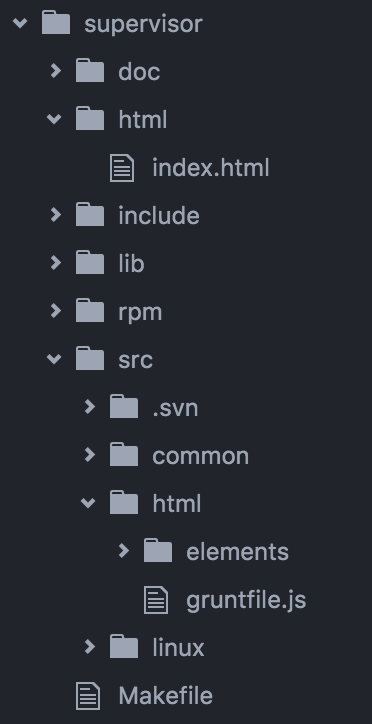
\includegraphics[width=.3\textwidth]{images/filetree}
  \caption{Trigger Supervisor folder stucture}
  \label{fig:filetree}
\end{figure}

\section{Separation of Concerns}
\label{Separation of Concerns}
SoC is a design primitive, dictating a modular design of the software. This has
been implemented in three ways.

Firstly, different syntaxes now are housed in their own files. This allows for
significantly less messy code and enables us to implement specific optimizations
for each language (for example a CSS pre- and post-processor).

Secondly, the developer is not limited to one source file for each syntax. If
circumstances would make some code easier to manage if it is housed across
multiple files this is now possible. An example of this would be a panel with
multiple specialized sections. Separating these sections will make the code
easier to read and maintain.

Thirdly, this approach pushes developers to separate data from markup. This is
a very good thing as it causes the code to once again be much more readable.
By having the C++ code only produce the necessary data and putting all rendering
and interaction on the front-end, developers can also safely replace rendering logic or
user interaction flow without having to worry about data generation.

\section{Grunt build system}
\label{Grunt build system}
During development of the front-end code. Code is kept in multiple files (for
the SoC principle).

Instead of loading all the separated files individually at runtime, they will
instead be compiled together at compile-time. This will improve loading speeds.
The tool used to do this is Grunt
\url{http://gruntjs.com/}, a task runner built on nodeJS that is used to process
front-end code languages. It is currently a popular tool to compile,
minify, lint, unit-test, etc. front-end code before it is put in production.
It has very wide community adoption, which results in a very rich set of tools
available for use.

Now that every code language is housed in specialized files, some
optimizations on them can run at compile-time. The main objective of these optimizations
is to achieve as much browser compatibility as possible.

\subsection{JavaScript processing}
In order to ensure compatibility with all required browsers all JavaScript code
is transpiled by Babel \url{https://babeljs.io/}. This will ensure that newer syntax,
like ECMAScript 2016 (ES7), will be transpiled into a more compatible equivalent.

Also the JavaScript code will be transpiled by UglifyJS
\url{https://github.com/mishoo/UglifyJS}. This will implement various code
optimizations\cite{UglifyJSCompressor} making the code faster.
% \subsubsection{Linting}
% \subsubsection{Transpilation of ES6}
% \subsubsection{Uglification}
\subsection{CSS processing}
\subsubsection{SASS}
Developers are given the possibility to write SASS code, an extension of the CSS
syntax, that will be transpiled into CSS on compile-time using libsass
\url{http://sass-lang.com/libsass}.

\subsubsection{Autoprefixer}
Also Grunt will automatically add vendor-specific prefixes to CSS properties to
maintain the required browser compatibility using a tool called autoprefixer
\url{https://github.com/postcss/autoprefixer}.
\subsection{HTML processing}
No processing is done on the html code except for the fact that it is inlined.
\subsubsection{Inliner}
Any css link tag or script tag is inlined (i.e. the contents of the referenced
file read and inserted in the document) when the url in that tag contains
`\_\_inline=true`.

\section{Templates}
To assist developers when creating new interfaces, a set of template files and
scripts have been developed.

Where appropriate, a script `new-element.js` is present. A developer can execute
this command to create a new element containing html, sass, and javascript code,
all with inline documentation and a demo page.

\section{Panel registration system}
An interface consists of multiple libraries. Each of these could possibly contain
element definitions (e.g. the AjaXell library has elements concerning things like
session management).

To allow any loaded library to declare its own Web Components, a panel
registration system is included in the AjaXell libary.

It allows a developer to register any custom elements he developed in his cell
like so:
\fvset{frame=single}
\begin{pyglist}[language=cpp,numbers=left,numbersep=5pt,fontsize=\small]
void <package-name>::Cell::init()
{
  getContext()->addImport("/<package-path>/html/elements/elements.html");
}
\end{pyglist}
\fvset{frame=none}
With the `elements.html` file containing element definitions, either in eager
loading or in lazy loading syntax.

\subsection{Eager loading and lazy loading}
Depending on the content of the `elements.html` file, the element definitions
will either be loaded eagerly (i.e. at page load time) or lazy (i.e. when they
are needed). Of course a developer is encouraged to implement the lazy loading
approach, as it will decrease initial page loading times.

The eager loading approach is a list of HTML imports.
\fvset{frame=single}
\begin{pyglist}[language=html,numbers=left,numbersep=5pt,fontsize=\small]
<link rel="import" href="my-first-element/my-first-element.html" >
<link rel="import" href="my-second-element/my-second-element.html" >
\end{pyglist}
\fvset{frame=none}

While the lazy loading approach consists of a custom function provided by AjaXell.
\fvset{frame=single}
\begin{pyglist}[language=html,numbers=left,numbersep=5pt,fontsize=\small]
<script>
var base = document._currentScript.baseURI;
base = base.substring(0, base.lastIndexOf("/") + 1);

LazyLoad({
  base: base,
  provides: {
    "my-first-element": "my-first-element/my-first-element.html",
    "my-second-element": "my-second-element/my-second-element.html"
  }
})
</script>
\end{pyglist}
\fvset{frame=none}

\chapter{Documentation}
Documentation is something commonly taken too lightly. The legacy panel system
contains little to no documentation.
This frustrates developers and inhibits any changes to the codebase, because
there might be this undocumented flow of code that will break and only found out
about much later.

Fortunately there are some tools not only to properly write documentation
, but also to encourage developers to write documentation as the codebase
evolves.

\section{Inline documentation}
Documentation regarding the description code itself is kept close to the code,
in the form of inline documentation.

This means most of the documentation will be housed along with with the source
code itself. The goal is to minimize separation of code and documentation as
this easily leads to inconsistencies between the two.

Advantages of inline documentation are the reduced chances for outdated
documentation and being able to enrich source code with typed annotations
\cite{JS_Annotations}.

Source code consists of C++, JavaScript, HTML, and CSS code. The inline
documentation described here is applicable to the last three.

\subsection{JSDocs}
The syntax used to document JavaScript code is called JSDocs and is currently
at version 3\cite{JS_Annotations}\cite{JSDoc}. It provides us with a rich set of expressions
enabling a developer to write documentation comparable to JavaDoc.

JSDocs has wide industry adoption for JavaScript projects. It is widely used to
make code more understandable, generate HTML documentation, or use it to generate
the large traditional developer manuals.

In addition to JSDocs there are specific points in the source code where a developer can
provide code examples and extra directives to document HTML and CSS code. This
is however a non-standard method since there is no standardized way to document
any of the other languages inline.

\section{Global level}
The global level is the highest level and is the only level where documentation
is separated from the source code.

\subsection{Goals}
The main purpose of this documentation level is to be an entry point for developers.
It will teach developers the basics of the codebase, why things need to be done
one way or the other, and will point them to lower-level documentation whenever
appropriate (such as which package or element could be useful for a particular
use case).

Where lower level documentation will only focus on how to get stuff done, this
documentation level also has the responsibility to show developers concepts like
Separation of Concerns (see chapter \ref{Separation of Concerns}) and modular thinking.

\subsection{Sphinx}
This global documentation level is built using Sphinx (\url{http://www.sphinx-doc.org/}).
It takes a set of wiki-like documents and converts them in various types of
resources (HTML, \LaTeX, \ldots).
This is primarily focused on HTML output, but the \LaTeX~version is included in
this document as appendix~\ref{appendix_sphinx}.

\label{Sphinx}

\section{Package level}
The global level gives an overview of the packages that are available to a panel
developer.
The package level lies under the global level and is the first automatically
generated level. It describes the package's content and its capabilities.

\subsection{Goals}
Primarily, this documentation level gives a quick overview of the content of a
package. It also points readers to additional resources like element-level
documentation, the repository where the source code is hosted, and live demos
where supported.

\subsection{Grunt}
This documentation is generated in the Grunt build cycle described in chapter
\ref{Grunt build system}.
It loads and interprets every component of the package and generates a summary
page giving a general overview and pointing to several useful resources for each
component such as the documentation on the element level, a link to the code
repository, and a link to a live demo of the component if available.

The code it uses to render this documentation is housed in the source code of
each component. It gets interpreted by Grunt and is then compiled in the package
documentation page.

An example of a package level documentation page is show in figure \ref{fig:packagedocumentation}.
\begin{figure}
  \centering
  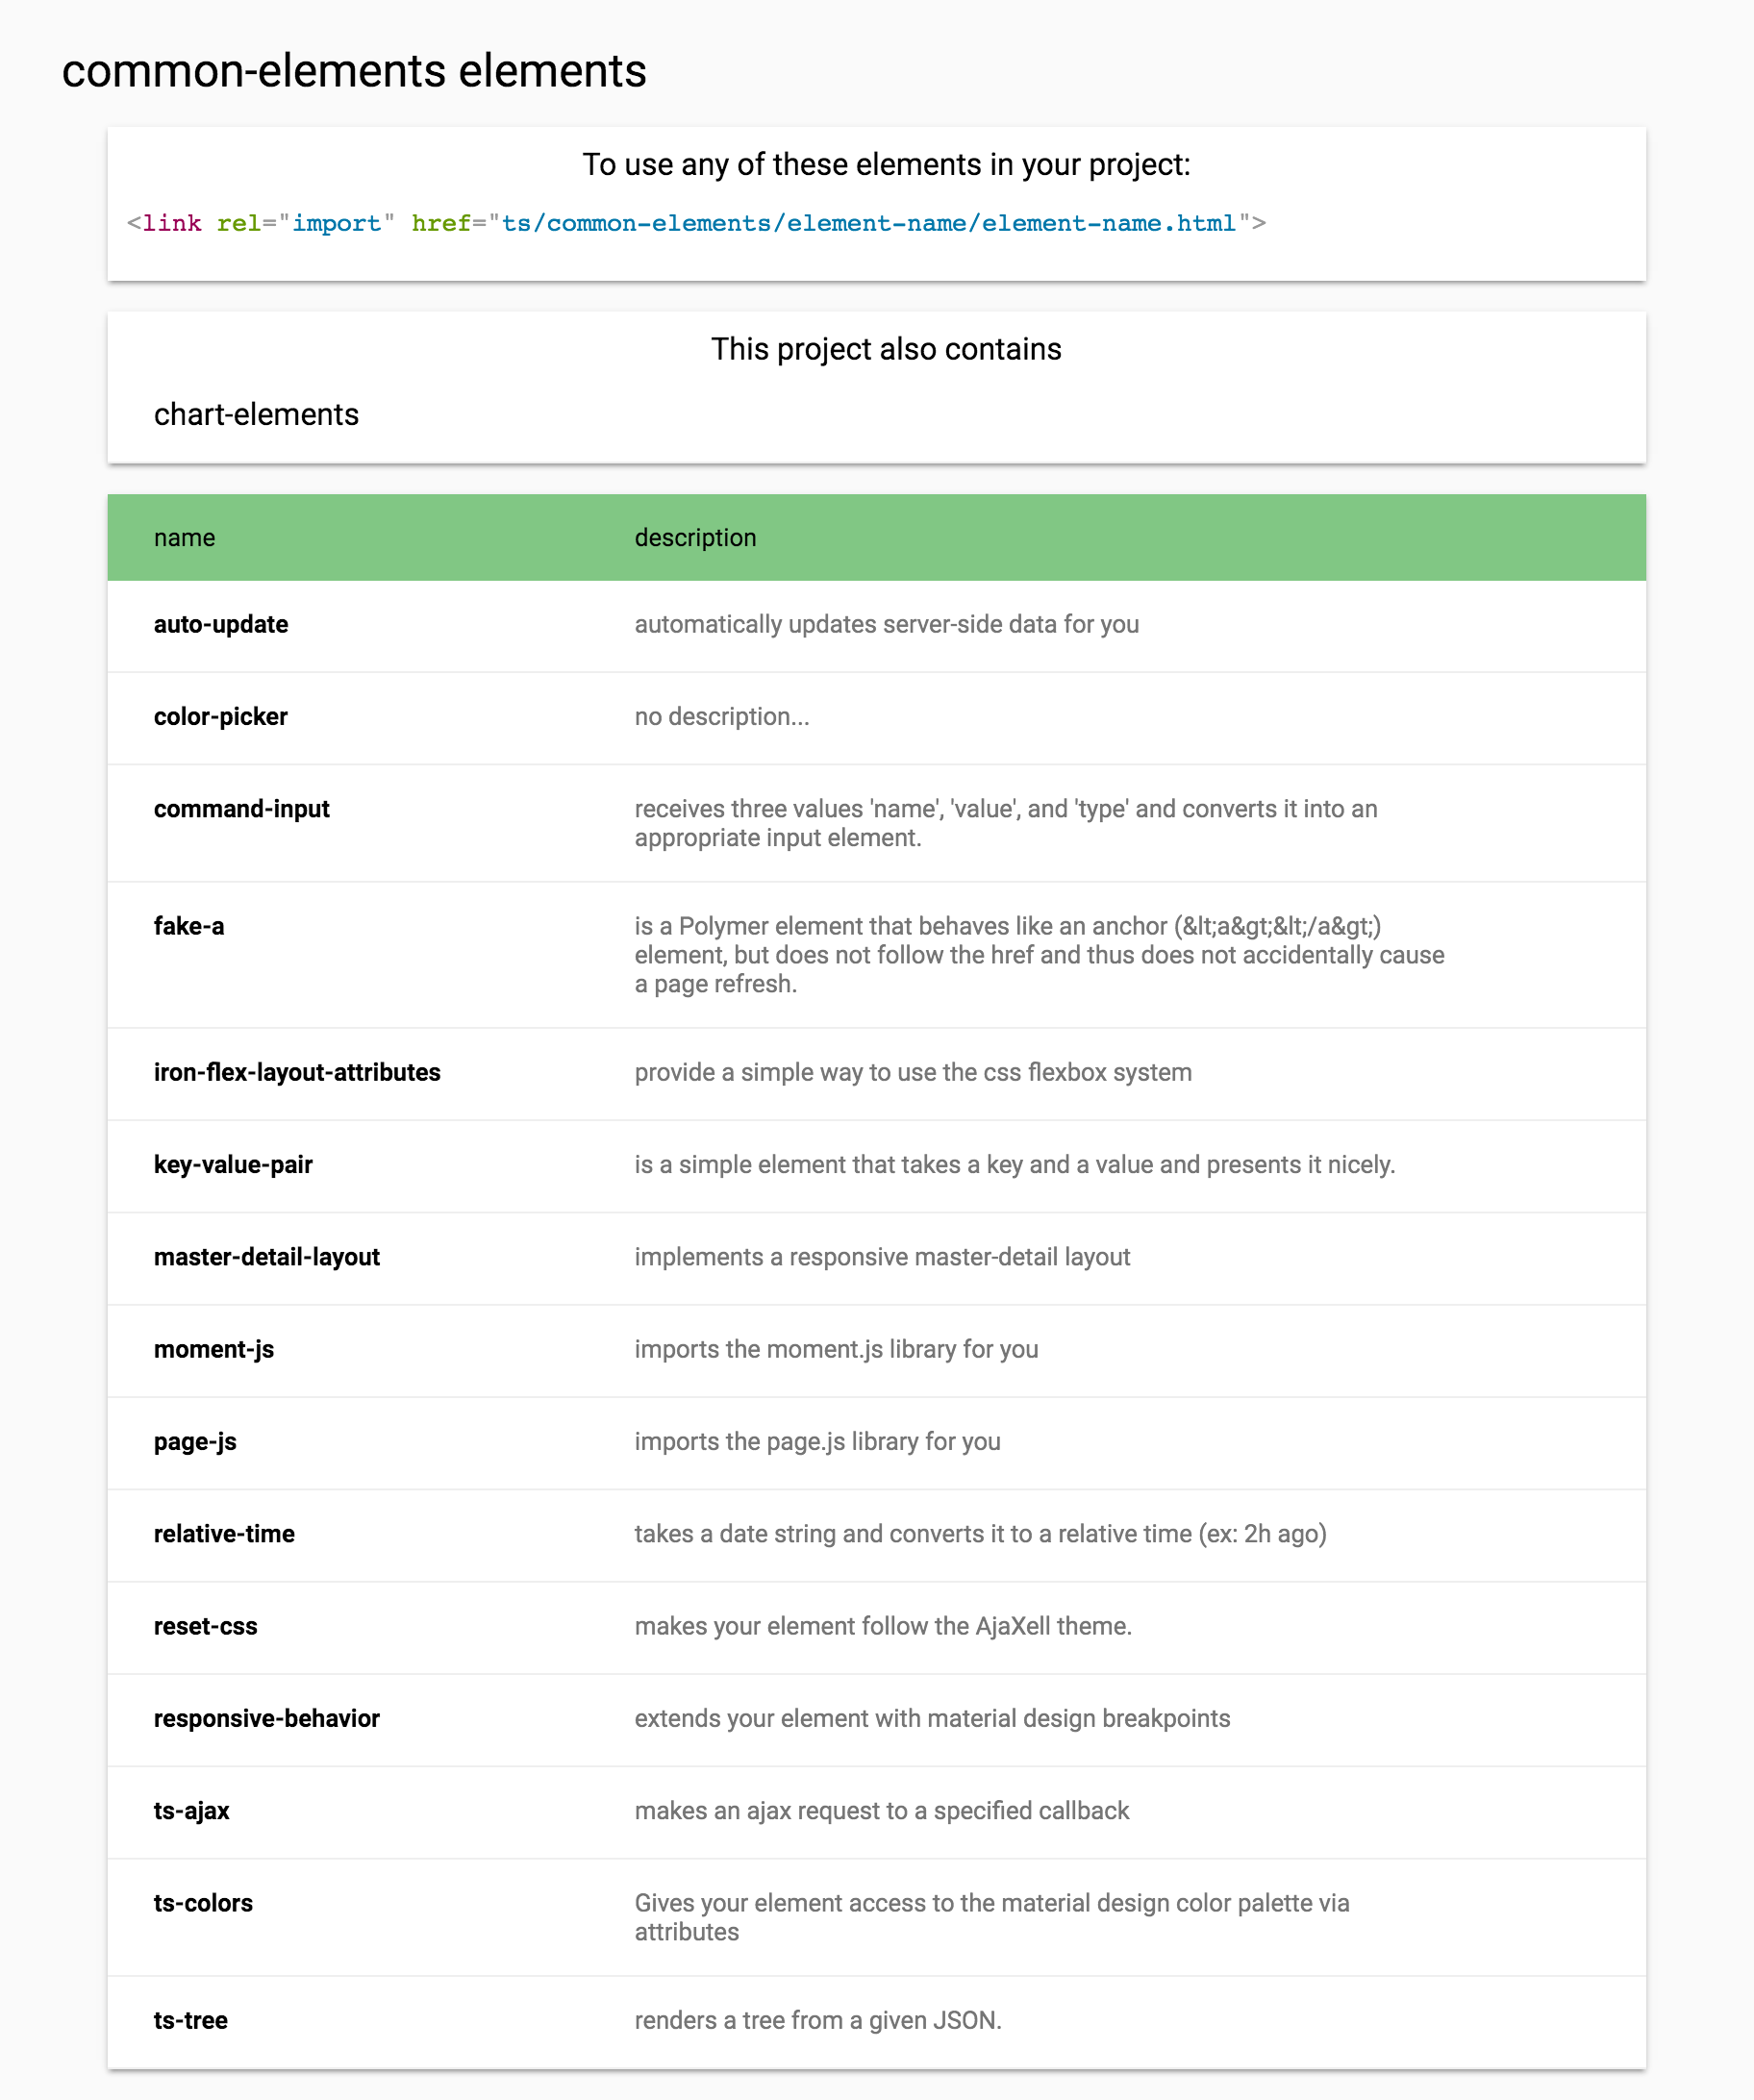
\includegraphics[width=\textwidth]{images/package-documentation}
  \caption{Documentation page of the common-elements package}
  \label{fig:packagedocumentation}
\end{figure}

\section{Element level}
The lowest level of documentation is documentation of individual web components.
This level is also auto-documented from the component's source code.
But unlike the documentation on the package level, where documentation is
generated on compile time, the documentation here is rendered on the fly, client-side.


\subsection{Goals}
This documentation provides an overview of all the properties and available
calls of this component. It can also provide code examples and even live
demos.

\subsection{iron-component-page}
Client-side rendering is done by using a specialized web component called `iron-component-page`
(\url{https://elements.polymer-project.org/elements/iron-component-page}).
It uses the `hydrolysis.js` library to interpret the inline documentation provided
by the developer in the source code of the web component, and compiles this into
a documentation page.

An example of an element level documentation page is show in figure \ref{fig:elementdocumentation}.
\begin{figure}
  \centering
  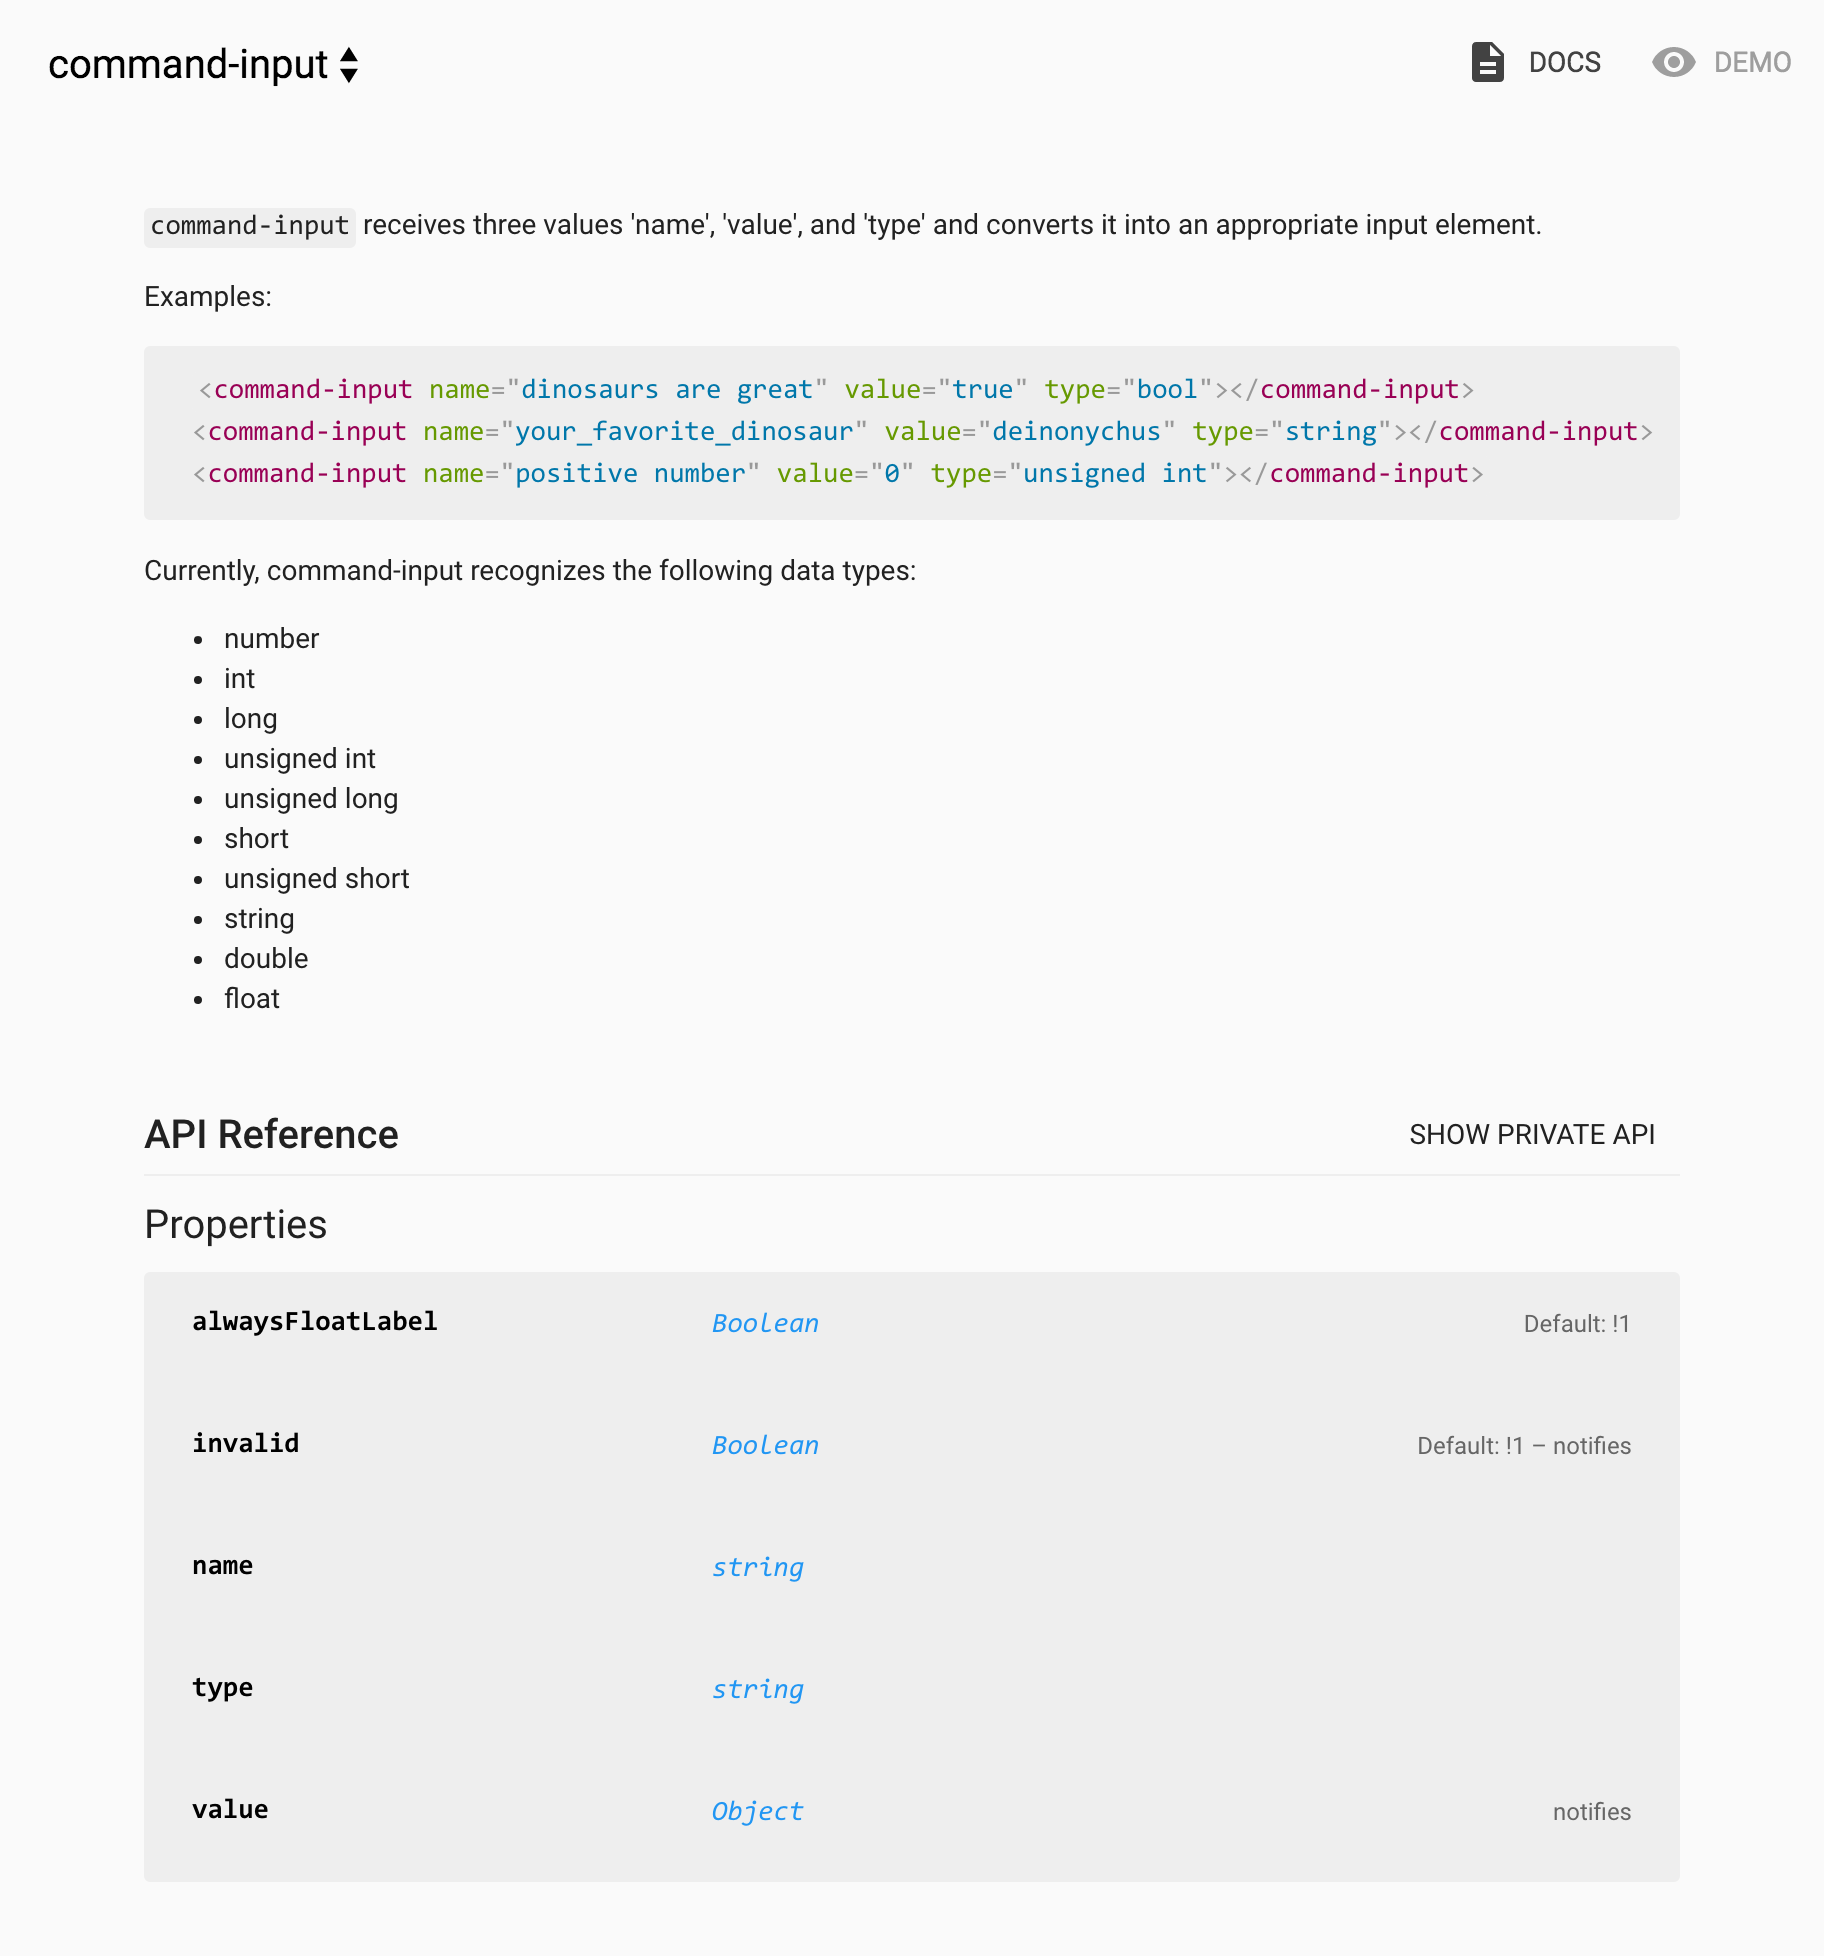
\includegraphics[width=\textwidth]{images/element-documentation}
  \caption{Documentation page of the command-input element}
  \label{fig:elementdocumentation}
\end{figure}

\chapter{Browser testing}
The TS interface officially supports the latest ESR release of Mozilla Firefox.
However, user tend to use many different browsers. When developing new interfaces
it is very unpractical to test all these browsers manually and consistently.

Also, because of the frequent changes made to web browsers (described in chapter \ref{Evergreen browsers}),
it has become very important to test interface functionality as browser versions
get updated at production systems.

\section{Selenium}
Selenium is a tool that can automate a browser. Its most common uses are to
perform tests or to automate web interfaces.

Starting from version 2, it uses an open standard called `WebDriver` to interact
with a browser. Most modern browsers have a native implementation of this standard,
and separate drivers exist for browsers that do not (including IE6).

Selenium can run under Windows, Mac OS X, and Linux (Debian \& RHEL).
It has official libraries for C#, Haskell, Java, JavaScript (Node.js), Objective-C,
Perl, PHP, Python, R, and Ruby.

\section{Web-component-tester}
The polymer project contains a dedicated testing tool to test Polymer elements and
is used in the TS.

It allows a developer to make a series of tests for every Polymer element (and thus
every interface). These tests are performed using the grunt build system when
executing `grunt test`.

Tests are defined in a `test` folder in the source folder of every element.
There a developer can define tests with the `test()` function like this:

\fvset{frame=single}
\begin{pyglist}[language=javascript,numbers=left,numbersep=5pt,fontsize=\small]
// this function tests if the Polymer element has declared an object
// `someObject` and it has a property `name` with value `deinonychus`
test('defines the "author" property', function() {
    assert.equal(element.someObject.name, 'deinonychus');
});
// tests if the function `sayHello()` returns a specific string.
// also tests if the function `sayHello()` respects its arguments.
test('says hello', function() {
    assert.equal(element.sayHello(), 'template-element says, Hello World!');
    var greetings = element.sayHello('greetings Earthlings');
    assert.equal(greetings, 'template-element says, greetings Earthlings');
});
\end{pyglist}
\fvset{frame=none}

More advanced use cases, such as testing AJAX (Asynchronous JavaScript And XML) requests
or even emulating an AJAX response are also possible.
More detailed examples of web-component-tester can be found in the Sphinx documentation,
which can be found in appendix \ref{appendix_sphinx}.

When a developer executes `grunt test`, a Selenium server is started and the
defined tests are performed using the latest version of Mozilla~Firefox,
Google~Chrome, Google~Chrome~Canary, and Safari (if possible).

\begin{figure}
  \centering
  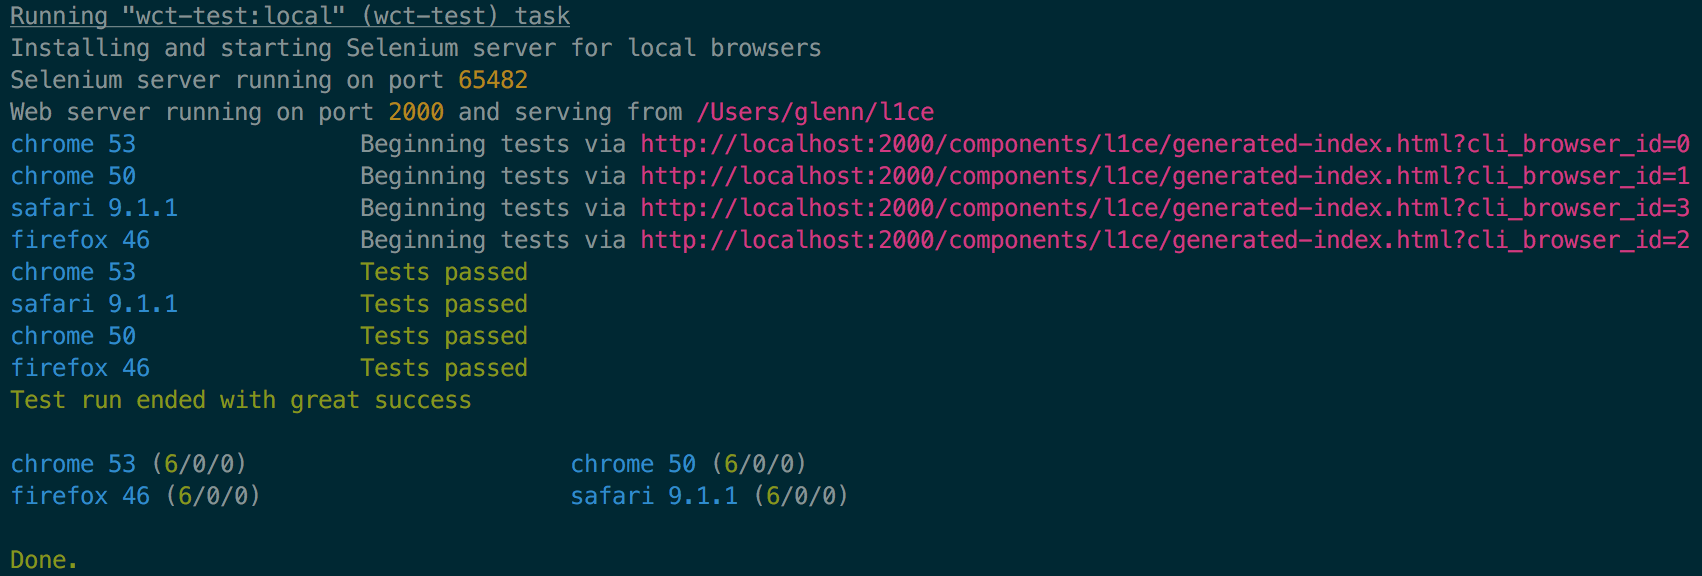
\includegraphics[width=\textwidth]{images/grunt_test}
  \caption{Console output when running tests with web-component-tester}
  \label{fig:grunt_test}
\end{figure}

\chapter{Results}


\section{Loading times}
\label{Loading times}
Table \ref{tbl:loadingtimes} shows an overview of the initial full page loading
times for the legacy TS (version 2.1.0) and the new TS (version 3.4.0). That is,
a page load from a new browser tab with all caches removed.

This test is performed with the timeline panel of Google Chrome 50.0.2661.86 (64-bit).

\begin{table}
  \begin{center}
    \begin{tabular}{| l | l | l | l | l |}
    \hline
     & TS 2.1.0 (Dojo) & TS 3.4.0 (Dojo + Polymer) & difference & difference (\%) \\ \hline
    \textbf{Loading} & 44.5ms & 112.4ms & +67.9ms & +152.58\%  \\ \hline
    \textbf{Scripting} & 1227.6ms & 1187.6ms & -40ms & -3,26\% \\ \hline
    \textbf{Rendering} & 29.7ms & 171.0ms & +141.3ms & +475,76\% \\ \hline
    \textbf{Painting} & 7.5ms & 36.1ms & +28.6ms & +381.33\% \\ \hline
    \textbf{Other} & 106.4ms & 335.9ms & +229.5ms & +215,69\% \\ \hline
    \textbf{Idle} & 213.6ms & 775.1ms & +561.5ms & +262,87\% \\ \hline \hline
    \textbf{Total} & \textbf{1.63s} & \textbf{2.62s} & \textbf{+990ms} & \textbf{+60,73\%} \\ \hline
    \end{tabular}
  \end{center}
  \caption{Page loading times for TS 2.x and 3.x}
  \label{tbl:loadingtimes}
\end{table}

It is expected that the TS 3.x has higher values for everything in this table,
because it loads two front-end libraries (Dojo \& Polymer).

Notable is the decrease of scripting time for the TS 3.x relative to the
TS 2.x. This is because Dojo is minified and packaged into one JavaScript file
in the TS 3.x release, where as in the TS 2.x release it was not.
Also, because this test is performed in Google Chrome, which has native support
for Web Components, very little scripting needs to be done.
This result will be different in other browsers like Mozilla Firefox, where
Web Components support needs to be emulated. Then again, the lazy loading system
largely removes this overhead from the initial page loading time, so only minor
differences would be expected here.

Rendering time has increased the most going from TS 2.x to TS 3.x. This makes
sense as Polymer renders everything on the front-end, whereas Dojo used to render
everything server-side.
During initial page load this rendering load is primarily caused by the rendering
of the left side menu.
The increase of painting time follows the same logic as the rendering time.

Also notable is the increase of idle time. This means that the browser needs to
wait for a task to finish before it can start another.
This is caused because the TS 3.x loads the default panel after the initial page
load. Which means the TS makes extra network request, to fetch an interface panel,
right after initializing. This is counted with the initial page load.
TS 2.x just shows a blank page, it loads no default panel.
Because the browser needs to wait for the extra network requests to finish before
it can render the default panel, the idle time goes up by a lot.

In total, the initial page loading time increased with about 60\%, which is an
acceptable increase given the new TS runs 2 libraries concurrently.

\section{CPU consumption}
Both TS releases have negligible CPU usage when doing a fresh page load, and
stay at 0\% CPU usage when the user is not interacting with the system.

TS 3.x uses hardware acceleration for it's animations since they are all made
using CSS transform properties or using Web Animations\cite{webanimations}.
The only exception to this is the `paper-spinner` element. Which displays a
loading animation.
The TS 2.x release did not have any animations.

% \begin{figure}[H]
%   \centering
%   
\includegraphics[width=.1\textwidth]{images/paper-spinner}
%   \caption{The most CPU intensive component of the TS 3.x interface}
%   \label{fig:paper-spinnger}
% \end{figure}

\section{Memory consumption}
Chapter \ref{Memory leaks in Dojo} described the memory leak problems in TS 2.x.
It showed a clear memory leak problem that needs addressing in TS 3.x.

Image \ref{fig:ts3_memory} showed that the new interface contains no memory leaks,
unless of course a panel developer creates one. This is why the `ts-ajax` and
`auto-update` elements in the `common-elements` package have been equipped with
ways to detect a circular reference, as they are the most likely to be used in one.

Unfortunately it also showed in figure \ref{fig:ts3_legacy_memory} that legacy
panels in the new TS still suffer from this memory leak. This is because the
circular references causing the memory leak reside in the Dojo library itself,
and thus would be impractical to address.
Therefore, any interface that included auto-refreshes had the highest priority
to be converted to a new TS 3.x interface.

Because TS 3.x uses client-side interface rendering rather than server-side as
the TS 2.x did, it uses more memory from the browser.

Chapter \ref{Loading times} already described that in TS 3.x the memory used
by an interface panel will be released after it switches to another panel.
It also described that in TS 2.x the memory consumption grows linearly with the
amount of panels loaded by the user.

To test the difference in memory consumption, both TS versions were opened in
a new tab while memory consumption is monitored. No panels are loaded, the
interfaces are just left for 120s. The mean memory consumption in those 120s is
then taken as the mean memory consumption for that TS release.
The results of this test are shown in table \ref{tbl:memoryusage}.

\begin{table}
  \begin{center}
    \begin{tabular}{| l | l | l |}
    \hline
     & Google Chrome & Firefox \\ \hline
    \textbf{TS 2.1.0 (Dojo)} & 20.051MB & 7.06MB \\ \hline
    \textbf{TS 3.4.0 (Dojo + Polymer)} & 24.564MB & 10.96MB \\ \hline
    \textbf{difference} & +4.513MB & +3.9MB \\ \hline
    \textbf{difference (\%)} & \textbf{+22.51\%} & \textbf{+55.24\%} \\ \hline
    \end{tabular}
  \end{center}
  \caption{Memory usage for TS 2.x and 3.x in Mozilla Firefox and Google Chrome}
  \label{tbl:memoryusage}
\end{table}

\section{Functionality}
TS 3.x has functionally more capabilities for the interface than TS 2.x had.
More importantly, the TS interface is now no longer bound to one framework.
Any Web Component can be used, and extra functionality can be developed in-house.
This unlike TS 2.x where developers were functionally bound to the elements the Dojo
developers provided.

This makes TS 3.x far more easy to change, and thus more ready for the future.

\section{SDK improvements}
The fact that multiple programming languages are no longer placed into one file,
but distributed across multiple files, makes the developing an interface panel
a lot easier.

The Web Components approach to build interfaces gives developers a set of
powerful tools that are easy to use and extend.
% \subsection{Decreased development time}

% \section{Documentation}

\section{Developed panels}
The Control Panels are a set of custom interfaces, developed for an individual cell.
The other panels however occur on every cell. And are upgraded as part of the
new TS release.
\subsection{Commands}
The new commands panel use the `command-input` element for its input. Making it
easily extendible to understand more input types (e.g. vectors).
Currently it understands number, int, long, unsigned int, unsigned long, short,
unsigned short, string, double, and float input.
\begin{figure}[H]
  \centering
  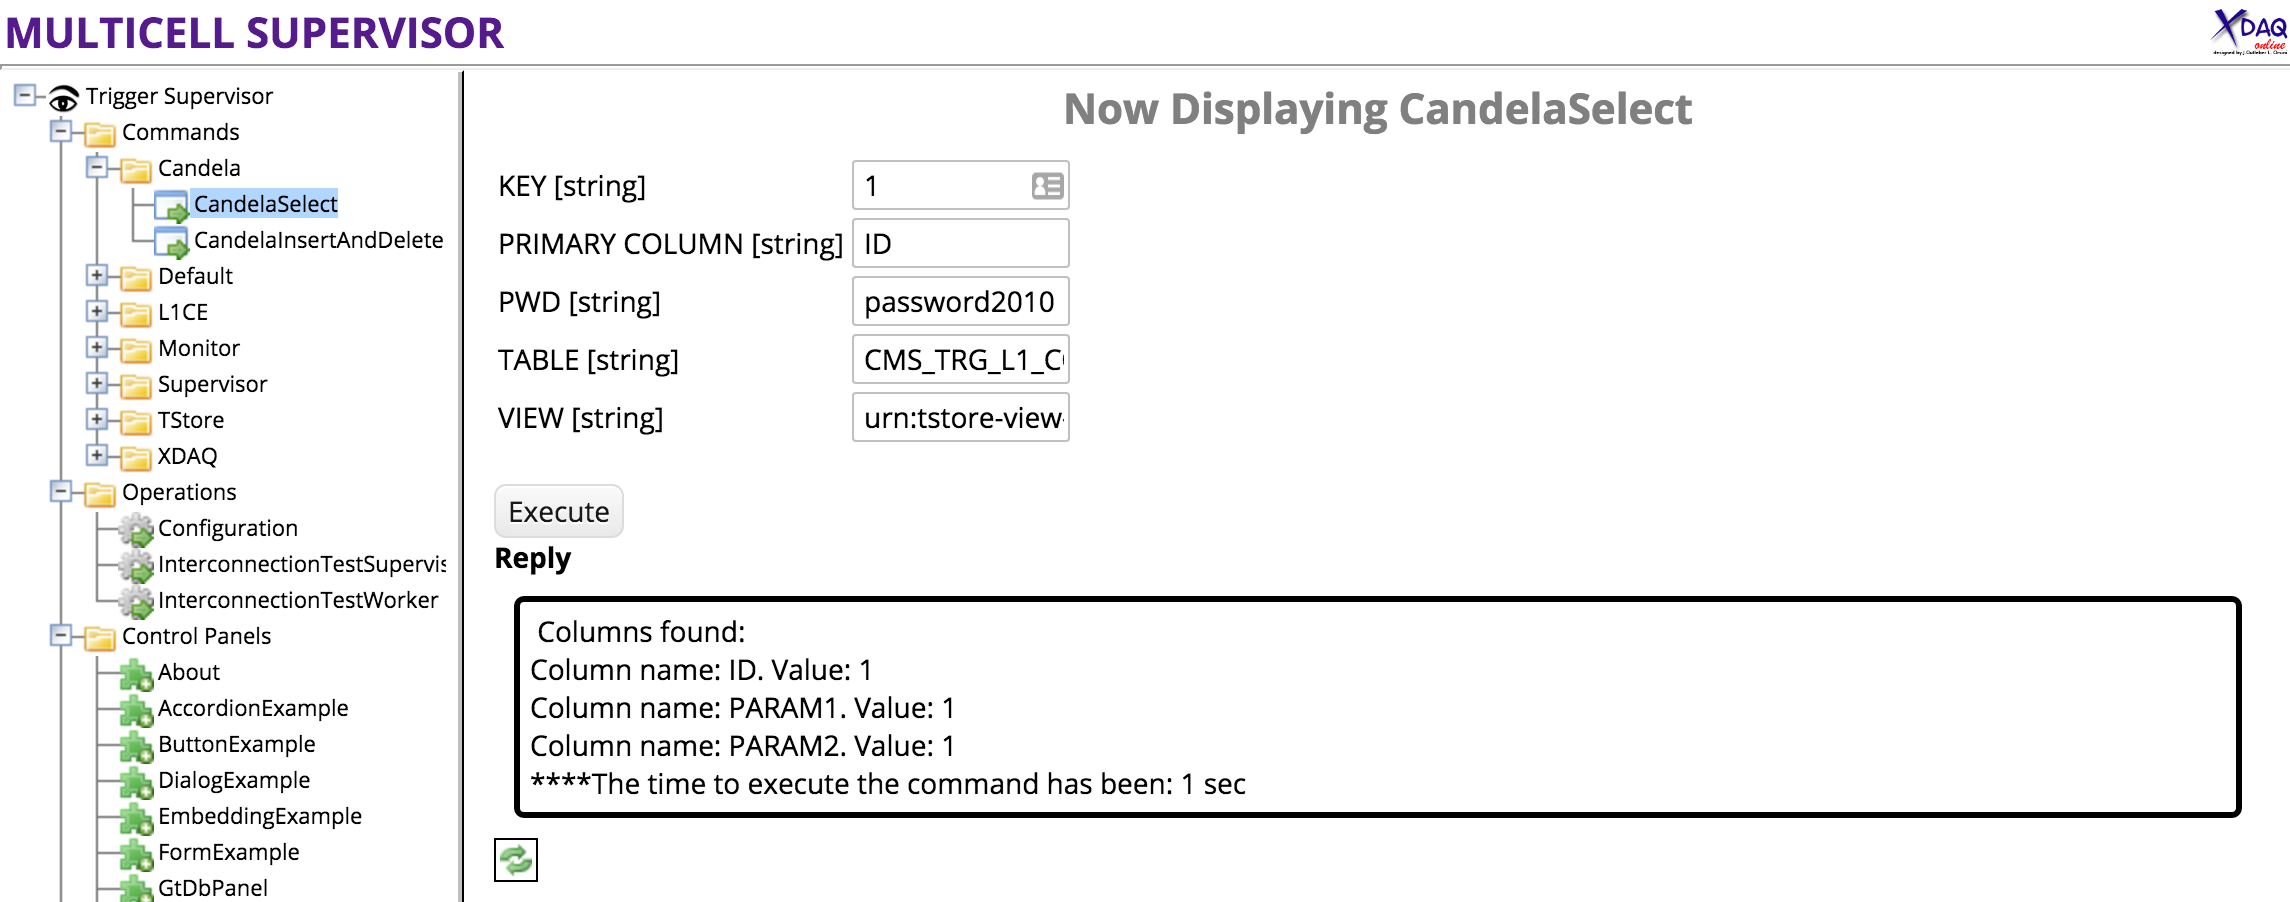
\includegraphics[width=\textwidth]{images/ts2_commands}
  \caption{TS 2.x commands panel}
  \label{fig:ts2_commands}
  \centering
  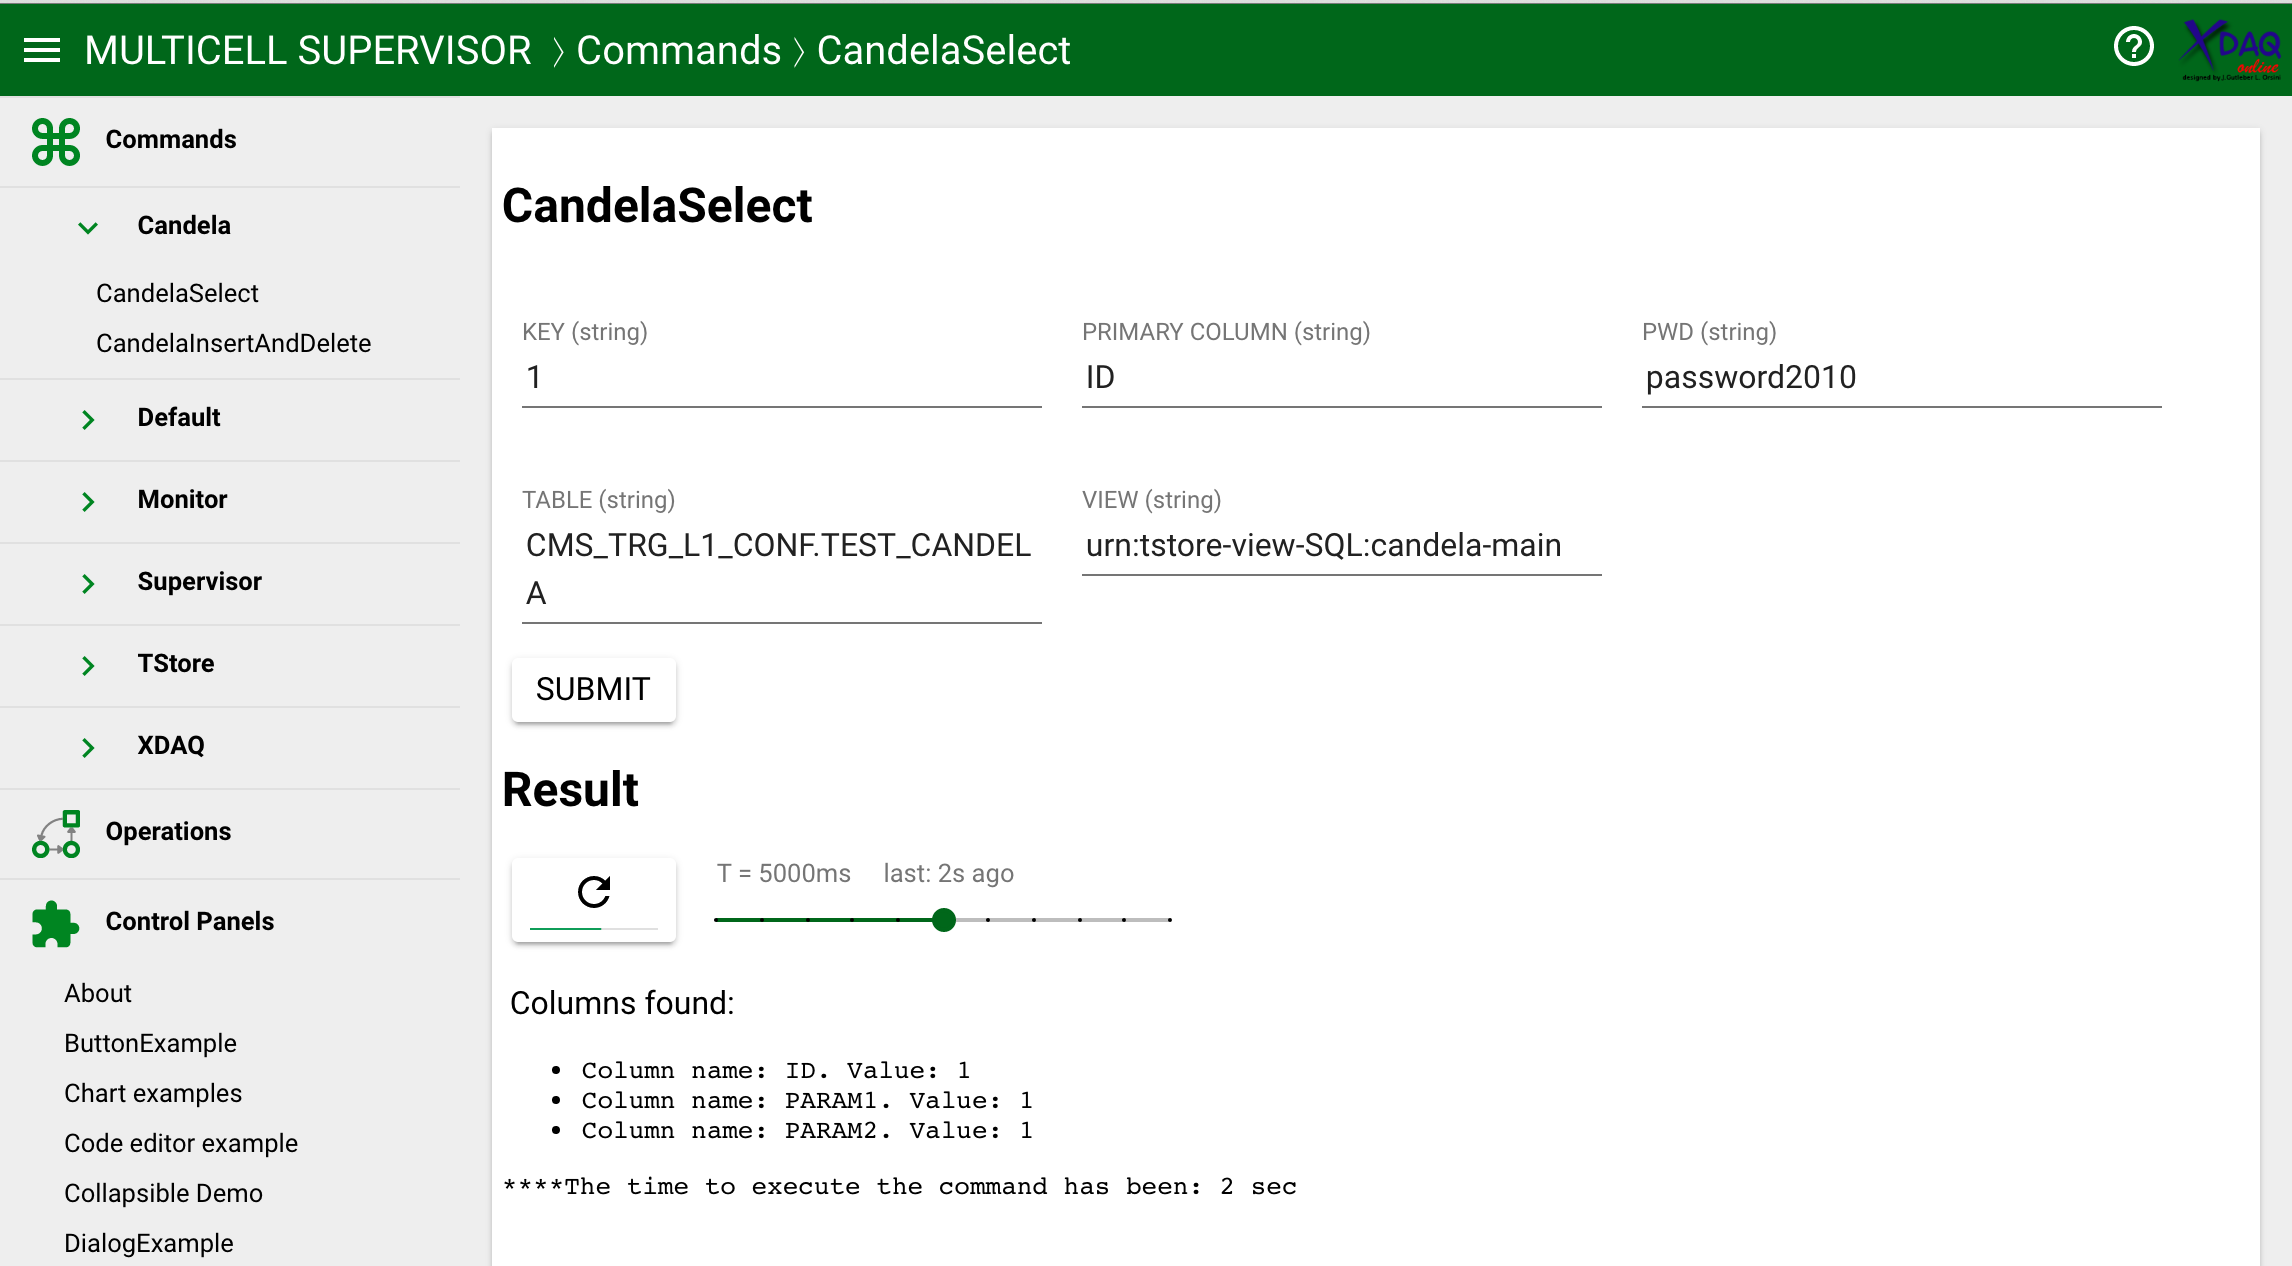
\includegraphics[width=\textwidth]{images/ts3_commands}
  \caption{TS 3.x commands panel}
  \label{fig:ts3_commands}
\end{figure}

\subsection{Operations}
The TS 2.x operations panel had some problems with auto-updating.
The state diagram tended to update very late, if it updated at all.
Result data and new available commands usually took more than 10 seconds to
show up in the interface.

The new operations panel is now far more responsive.
The state diagram is available when clicking on an icon, as it was deemed a
waste of space to show it by default.
\begin{figure}[H]
  \centering
  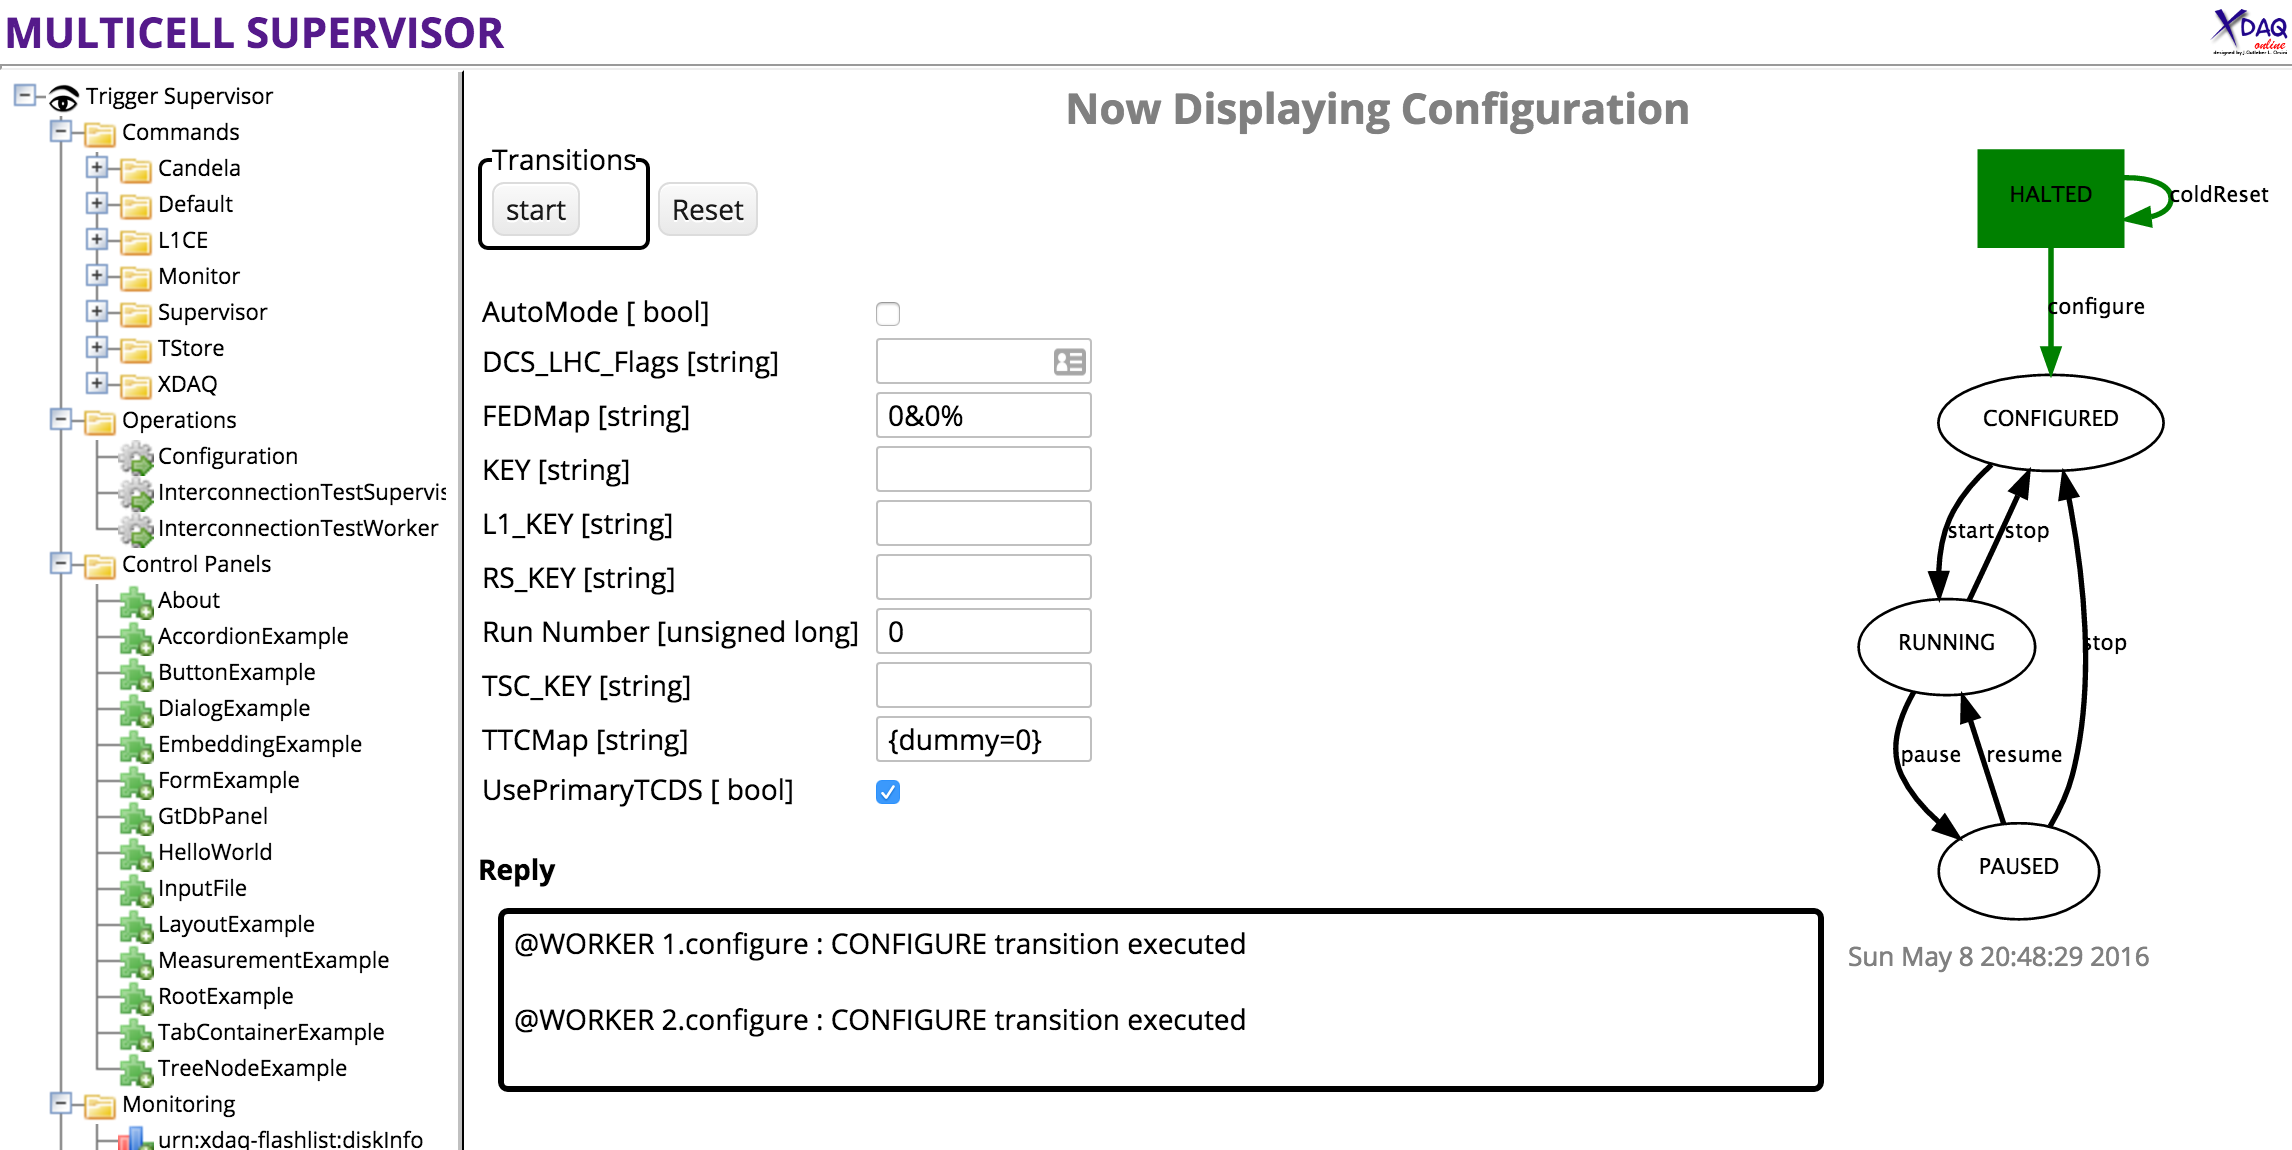
\includegraphics[width=\textwidth]{images/ts2_operations}
  \caption{TS 2.x operations panel}
  \label{fig:ts2_operations}
  \centering
  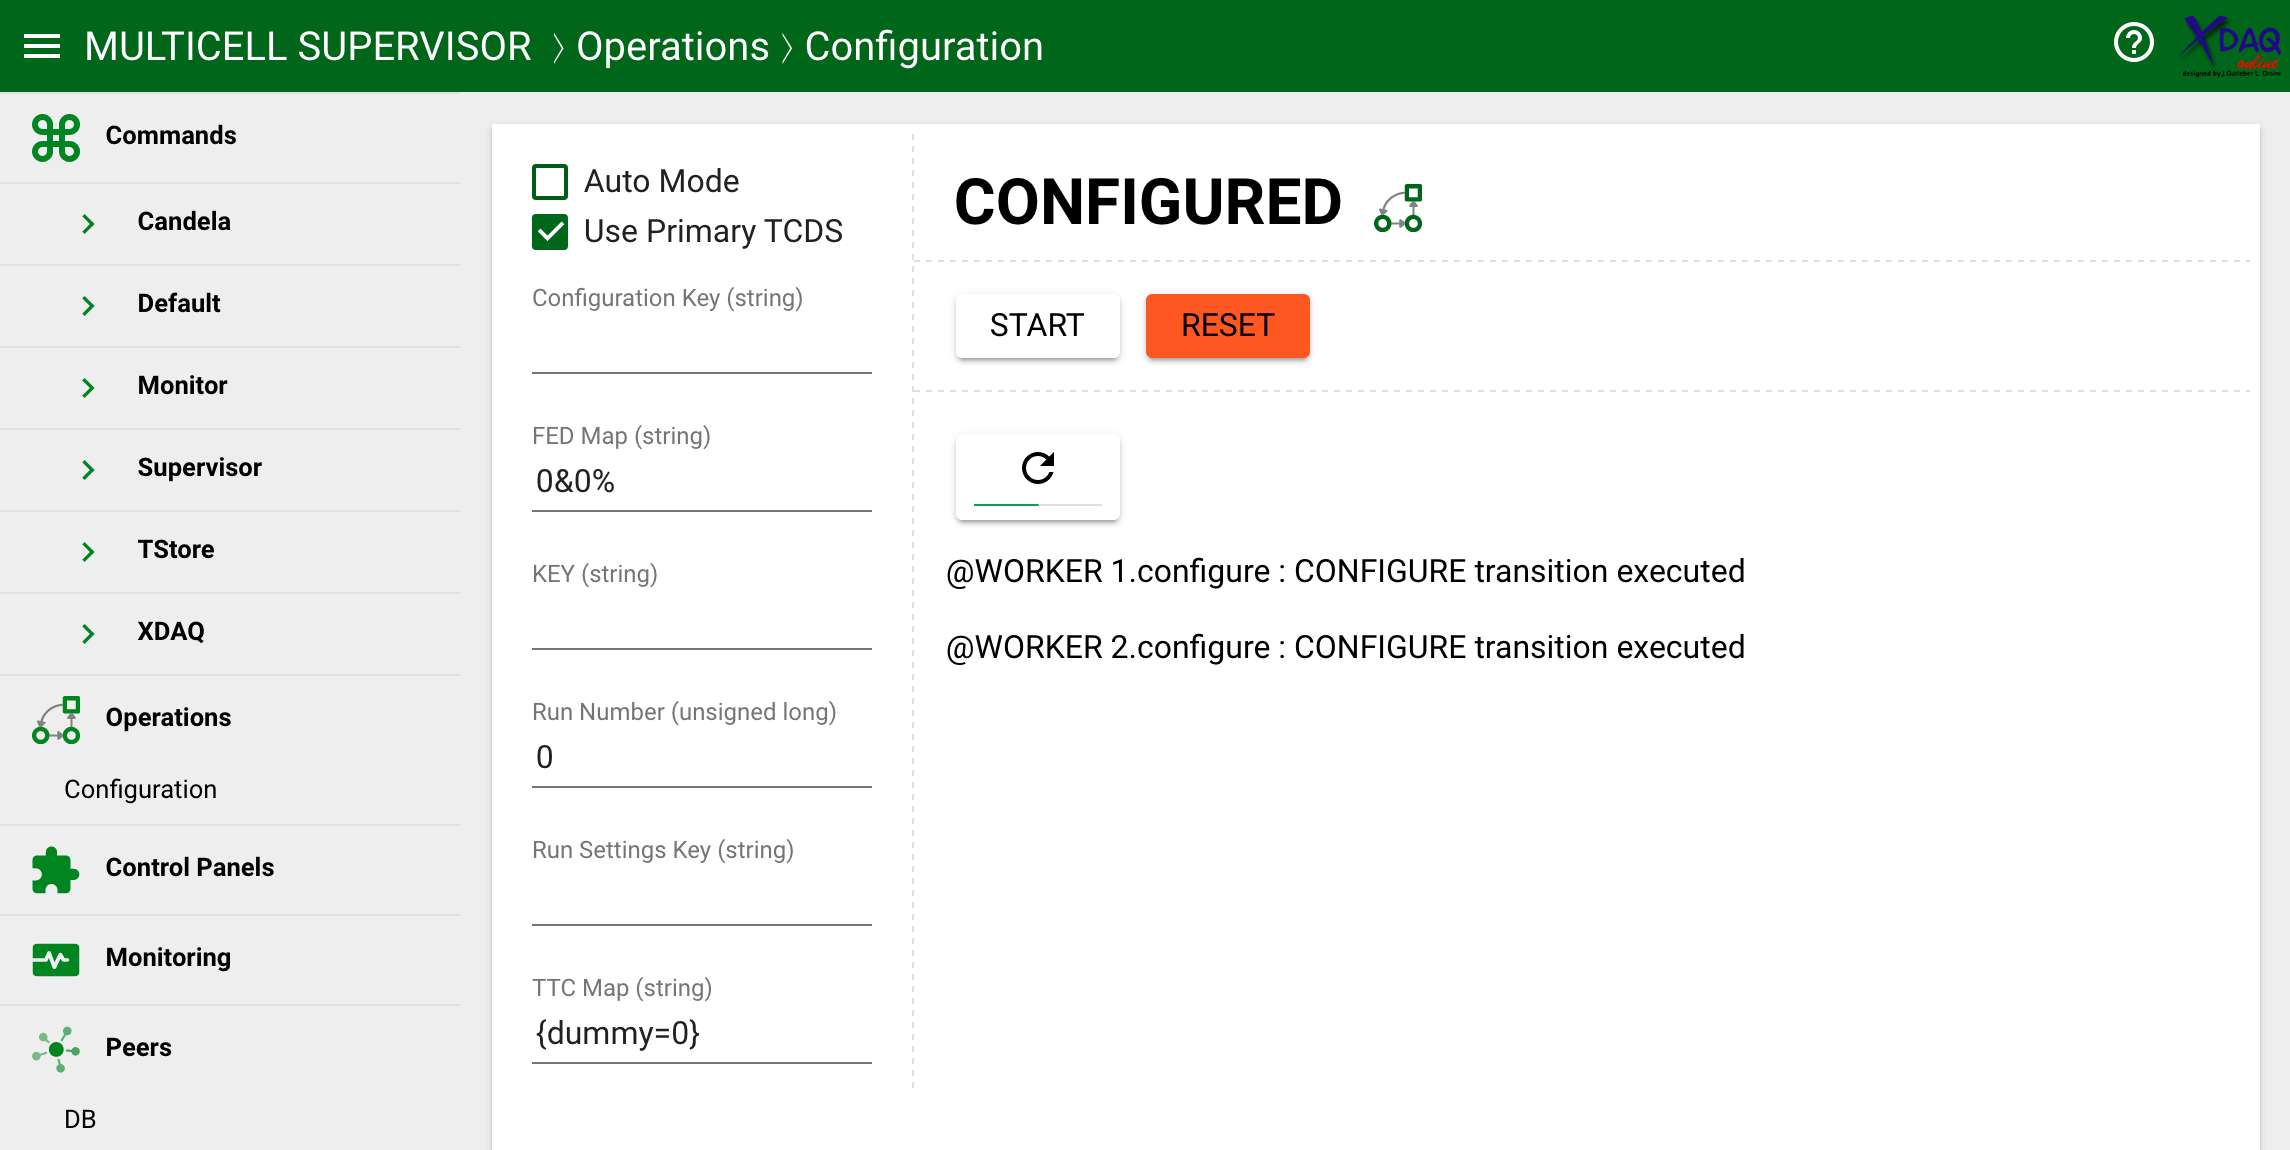
\includegraphics[width=\textwidth]{images/ts3_operations}
  \caption{TS 3.x operations panel}
  \label{fig:ts3_operations}
\end{figure}

\subsection{Flashlists}
% TODO definition of a flashlist
A flashlist is a more abstract interface designed to display tabular data.
This data can change with a regular interval. A table cell can contain a string,
date, number, or another table.

The flashlist panels now have a user-configurable auto-update function.
The flashlist can deploy custom renderers in the table depending on the data type,
for example a date will be shown as relative time (e.g. 9 minutes ago), instead
of just showing a time stamp. This list of custom renderers can be extended
easily.

\begin{figure}[H]
  \centering
  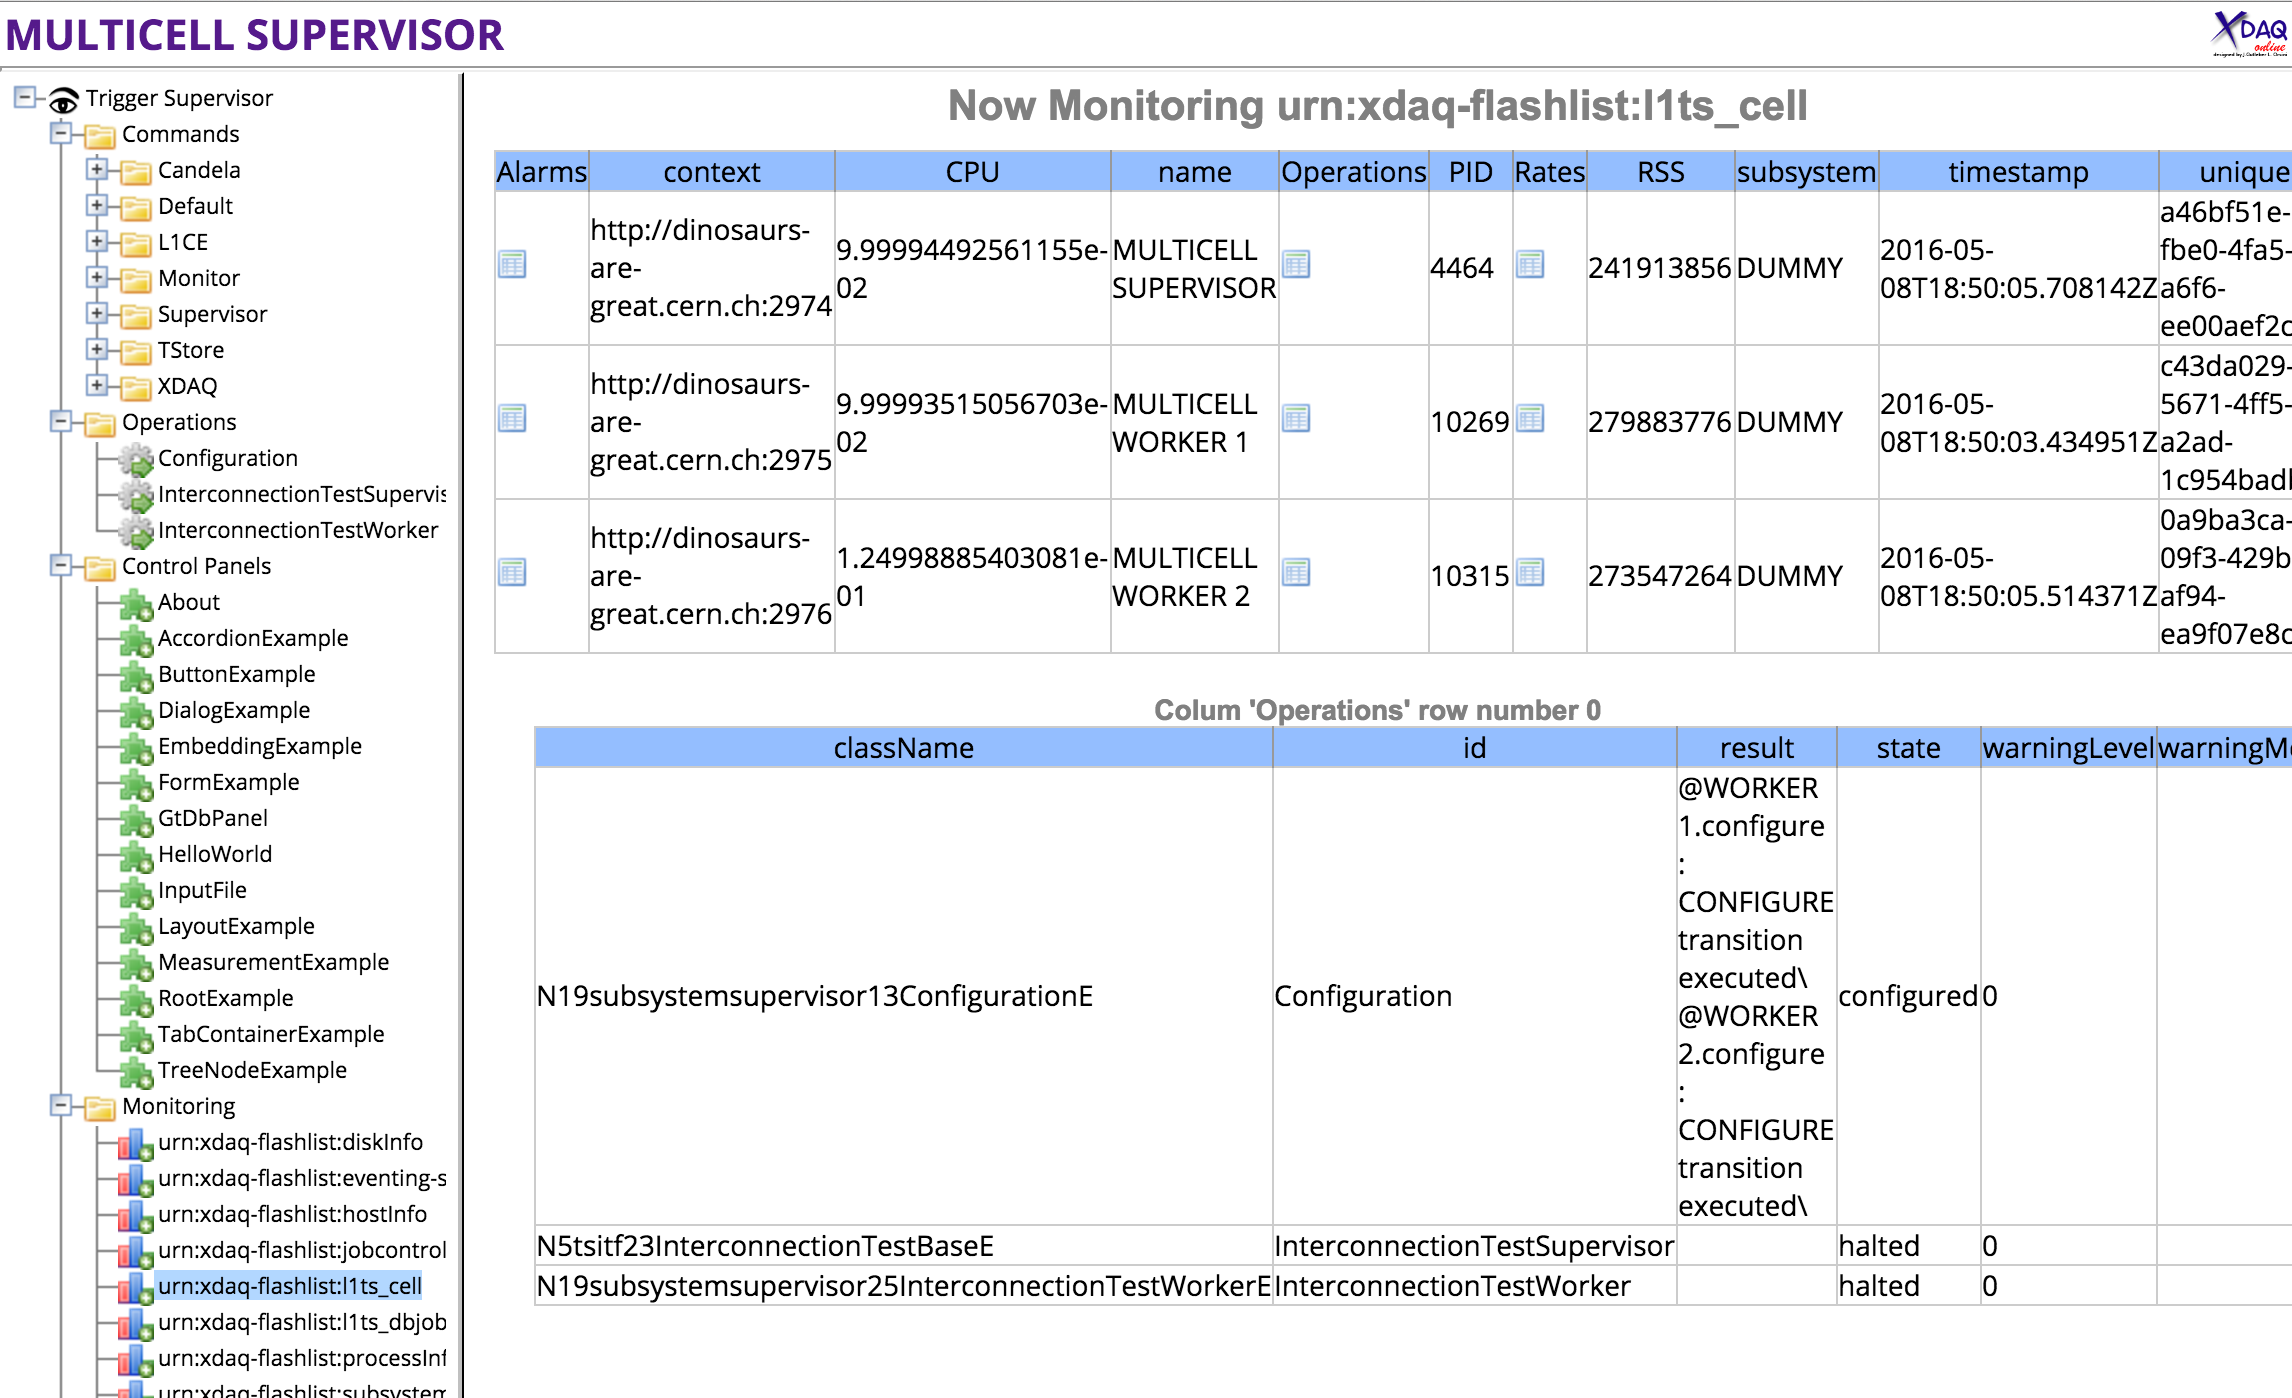
\includegraphics[width=\textwidth]{images/ts2_flashlists}
  \caption{TS 2.x flashlists panel}
  \label{fig:ts2_flashlists}
  \centering
  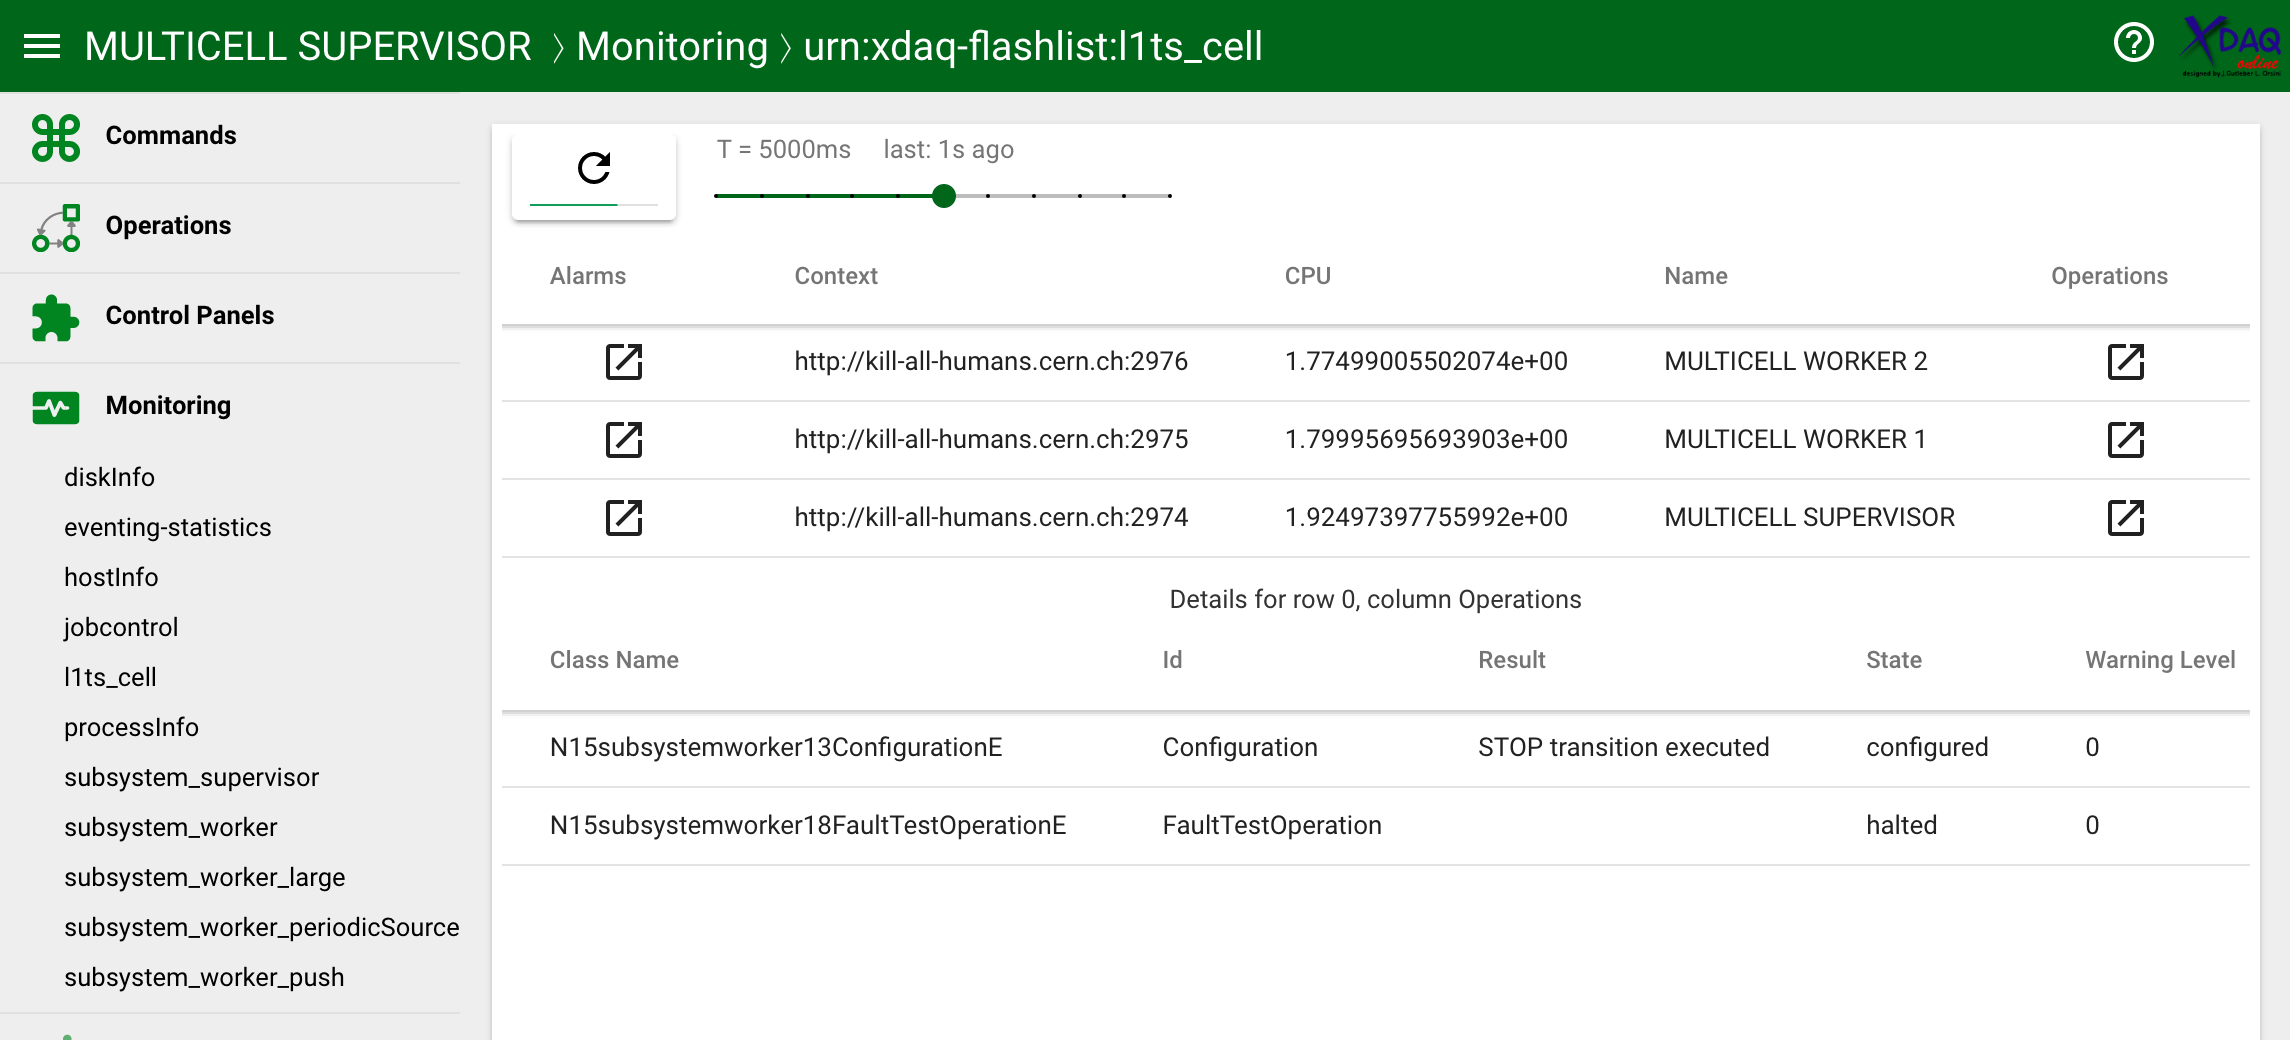
\includegraphics[width=\textwidth]{images/ts3_flashlists}
  \caption{TS 3.x flashlists panel}
  \label{fig:ts3_flashlists}
\end{figure}
% \subsection{Demos}

\chapter{Future}
A lot of big software projects (such as the Level-1 Configuration Editor and
the Level-1 page) rely on the TS.
Some of these projects are starting to benefit from the changes made to the TS,
and some of them are scheduled for a complete overhaul using the TS redesign as
a template.

Some things did not make it into the TS, because of backward-compatibility problems
or time issues.
However, as time goes on, the need to keep compatibility with legacy systems will
fade away. And some improvements may yet become possible.

\section{Dojo-free TS release}
At some point, all legacy (Dojo) panels will have been migrated to Polymer.
When this has occurred, legacy code can be removed from the TS.

A lot of code can be removed. The Dojo component classes, legacy session logic,
the legacy event system, etc.

Furthermore, Dojo can be removed from the front-end interface. This is expected
to bring a noticeable speed improvement to the initial page load.

At this point, the TS can also be prepared to take on a next framework, where this
time Polymer will be considered legacy code.

\section{HTML5 WebSocket}
A WebSocket is a full-duplex HTTP-like connection between a web browser and a web server.
Both the client and the server must support this protocol before such a connection
can be set up.

This allows for very efficient communication between client and server, and will
be especially useful when the server has frequently changing data to serve to the
client.
Traditionally this has been achieved using various sort of polling, which puts
unnecessary load on the server and the network.

This connection will also allow the web browser to receive updates near-instantaneous.

Currently, the most CPU intensive tasks in the TS interface belong to the auto-update
logic. This would be drastically reduced when implementing WebSockets.

\section{PRPL}
The PRPL\cite{PRPL} pattern is a software pattern for web apps designed by Google and stands for:
\begin{itemize}[noitemsep]
\item \textbf{Push} critical components for initial page load
\item \textbf{Render} the initial page
\item \textbf{Pre-cache} other components of the interface
\item \textbf{Lazy-load} needed components
\end{itemize}

It uses Web Components, HTML Imports, Service Workers, and HTTP/2 to accomplish
all these. The TS already uses two of them, Web Components and HTML Imports.
The two others that didn't make it into the TS are explained here in a bit more
detail.

\subsection{HTTP/2 Server Push}
Using HTTP/2, the server can interpret requested resources and decide to not only
return the requested resource to the client, but also provide the user with
additional resources related to the requested resource.

This is useful on the first page load, where a web browser requests the initial
page (usually `index.html`). This file very often contains references to other
resources such as CSS or JavaScript files.
Normally the web browser needs to make another request for each of these
resources.
HTTP/2 can multiplex these related resources along with the originally requested
resource over the same connection.
This severely reduces network latencies, as everything is returned
in one payload.
This effect is demonstrated in image \ref{fig:http1_server} and \ref{fig:http2_server}.

\begin{figure}
  \centering
  \begin{minipage}[t]{0.49\textwidth}
    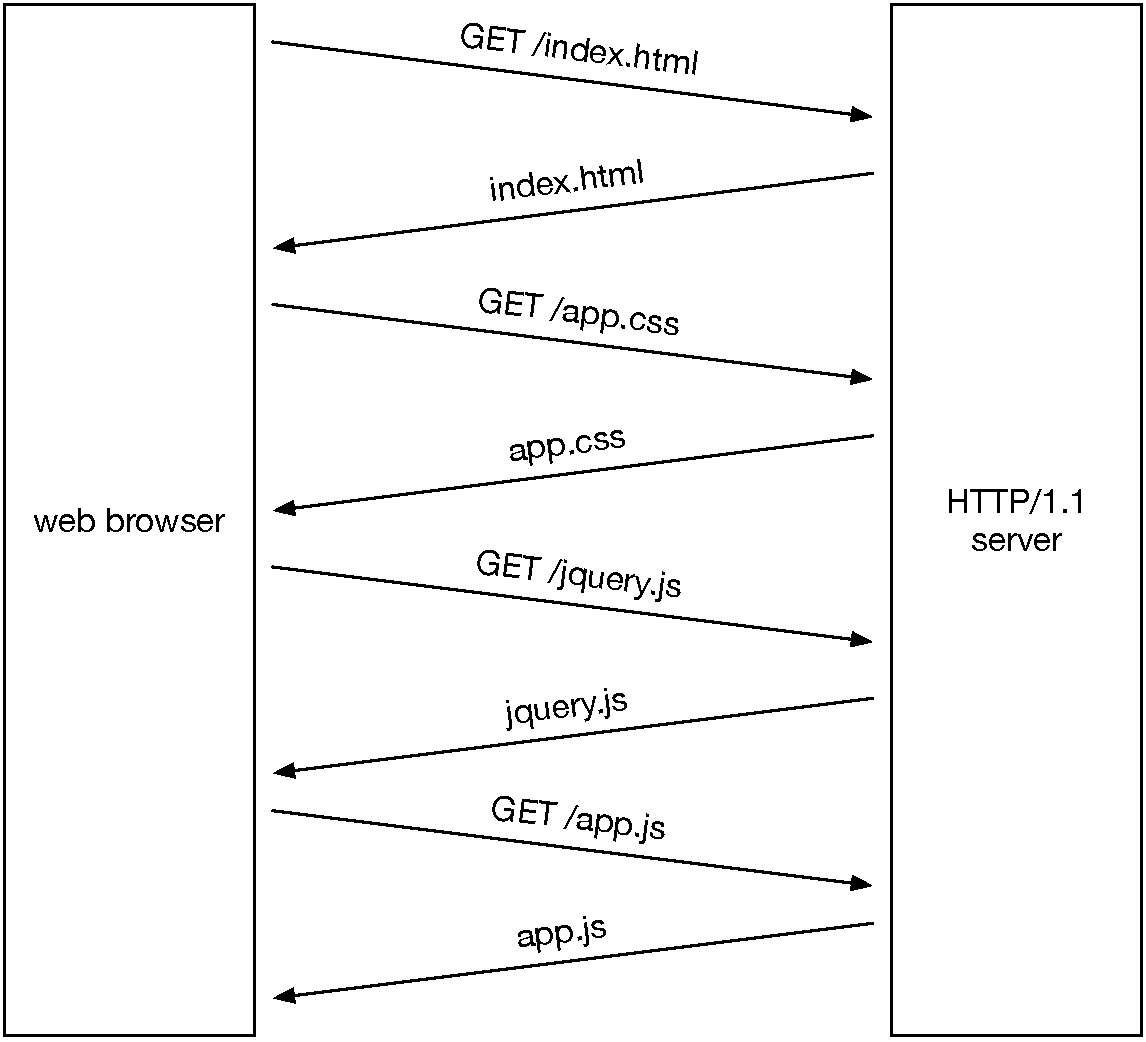
\includegraphics[width=\textwidth]{images/http1_server}
    \caption{A common request/response diagram when using a HTTP/1.1 server}
    \label{fig:http1_server}
  \end{minipage}
  \hfill
  \begin{minipage}[t]{0.49\textwidth}
    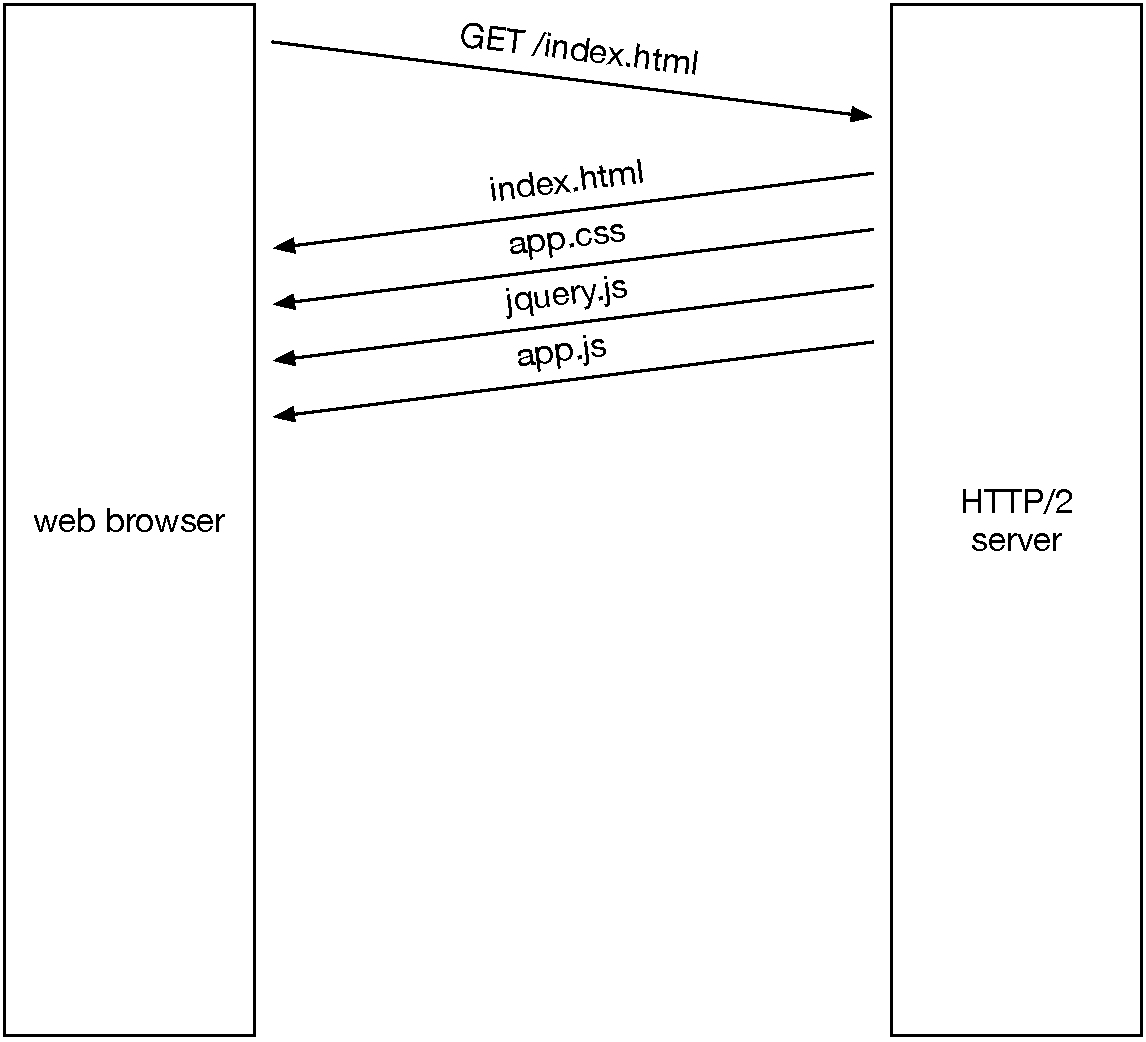
\includegraphics[width=\textwidth]{images/http2_server}
    \caption{A common request/response diagram when using a HTTP/2 server with Server Push}
    \label{fig:http2_server}
  \end{minipage}
\end{figure}

\subsection{HTML5 Service Worker}
A Service Worker is a JavaScript file that is run in the browser as a separate
thread.
Unlike traditional JavaScript files, this file has no access to the DOM or any
global variables like `document` or `window`. This file runs on a different scope.

A Service Worker runs in between the browser and the network. It is able to
intercept requests and modify them. It can even provide a response, thereby
completely bypassing the server and the network.

It also has full control over the browser cache. So the interface can programmatically
control what is put in the cache and when it is served or renewed.
This is shown visually in image \ref{fig:service_worker}.

\begin{figure}
  \centering
  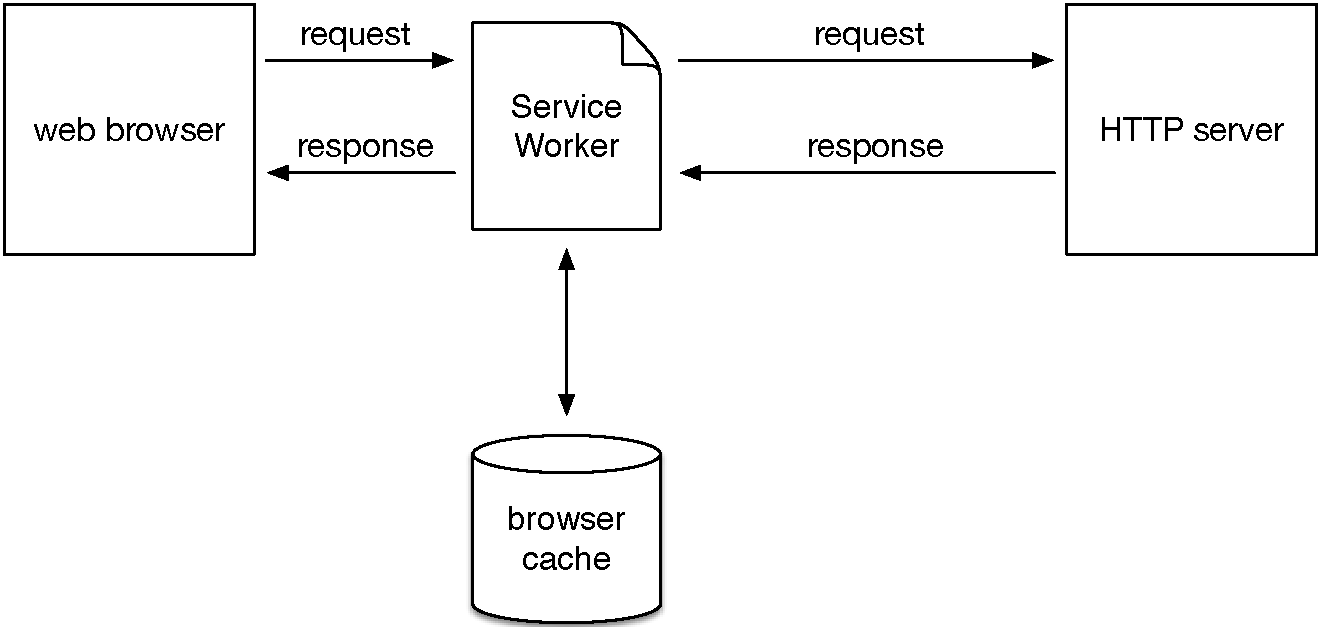
\includegraphics[width=\textwidth]{images/service_worker}
  \caption{Logical location of the Service Worker in a web browser}
  \label{fig:service_worker}
\end{figure}

This enables the interface to do two thing that were previously impossible, but
very useful.

The first is pre-caching. When the initial page load is done, the Service Worker
can silently pull resources from the web server before they are actually needed.
This will make interacting with the application a lot faster.

The second thing is offline functionality, and is a more elaborate version of
pre-caching.
When enough resources are pulled into the cache, the interface does not need the
web server anymore: in some cases (including the initial page load), the interface can work without an internet connection.

This will completely remove the need for network requests (except for receiving
new data): static resources (and data) are kept client-side and do not put a
load on the network anymore, vastly increasing performance.

\chapter{Conclusion}
The main objective was to upgrade the TS to be able to provide more advanced
interfaces, and to keep compatibility with legacy interfaces.

The new interface engine has achieved 100\% backwards compatibility, while
providing a completely new way to develop new interfaces.

This new interface engine and can be easily extended and is ready for any future
use-cases as it is built to change. The developers are not bound to the
functionality of one framework, rather it is build on open standards and thus
ensures maximum compatibility with future technologies.

The interface developers now have internal, semi auto-generated, documentation
at their disposal and have an active community on the world wide web to fall
back to.


% Bibliografie: referenties. De items zitten in bibliografie.bib
%%%%%%%%%%%%%%%%%%%%%%%%%%%%%%%%%%%%%%%%%%%%%%%%%%%%%%%%%%%%%%%%%
% Indien je ook de niet geciteerde werken in je bibliografie wil opnemen, commentarieer dan onderstaande regel uit!
%\nocite{*}
% \bibliographystyle{apalike}
% \nocite{*}
\bibliographystyle{IEEEtran}
\bibliography{chapters/bibliografie}

% Eventueel enkele appendices
%%%%%%%%%%%%%%%%%%%%%%%%%%%%%%
\appendix
% \chapter{Een aanhangsel}
sdfsffqsfsf

% Bijlage met daarin het wetenschappelijk artikel
%%%%%%%%%%%%%%%%%%%%%%%%%%%%%%%%%%%%%%%%%%%%%%%%%%
% \chapter{CMS TS Project}
% 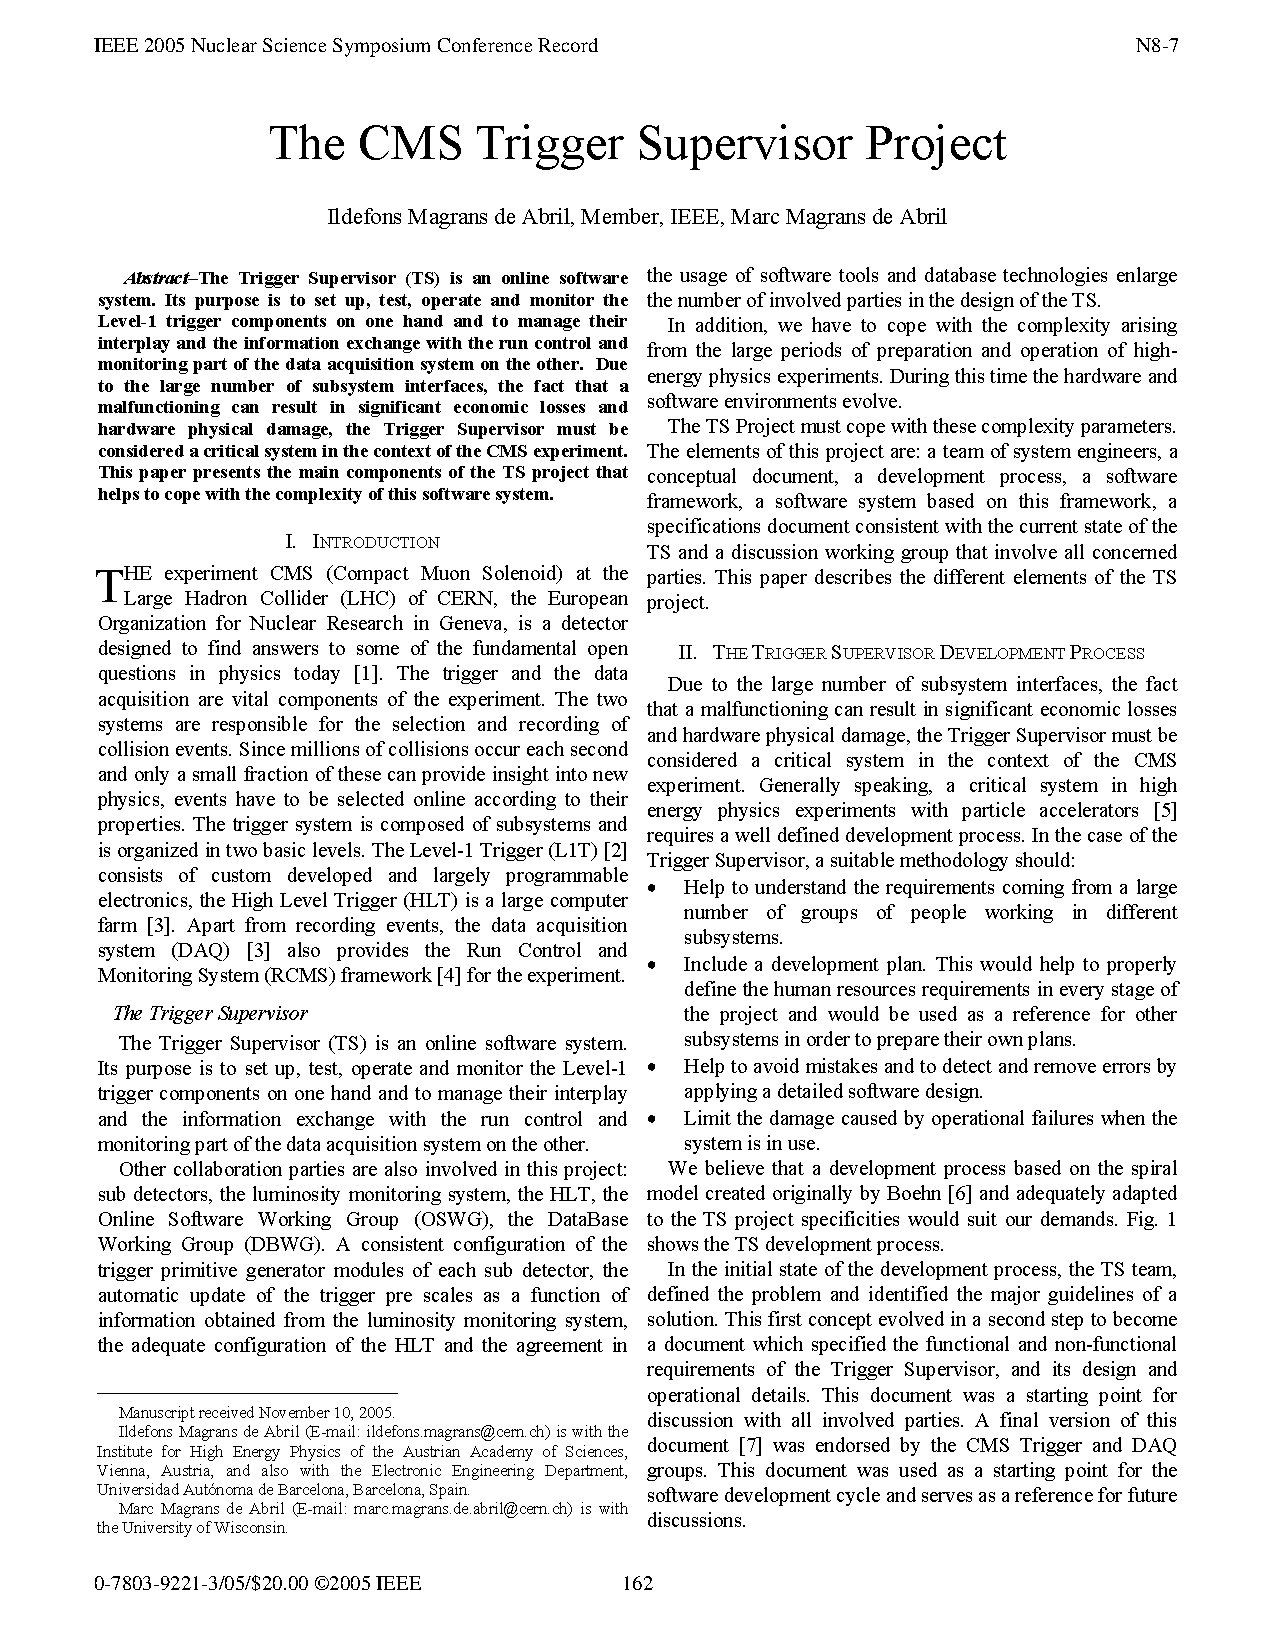
\includepdf[pages={1-}]{attachments/2005cms_ts_project_nss.pdf}

% Bijlage met daarin de poster
%%%%%%%%%%%%%%%%%%%%%%%%%%%%%%%
% \chapter{Poster}
%\includepdf{poster.pdf}

\chapter{Sphinx Documentation}
\label{appendix_sphinx}
Most part of the documentation of this project is auto-generated.
The manual documentation, developed in Sphinx (described in chapter \ref{Sphinx}),
is enclosed as an appendix to this document.
\cleardoublepage
\includepdf[pages={1-}]{TS_Documentation.pdf}

\chapter{Paper}
As part of this master thesis it was required to write a paper on the subject.
A copy of this paper is enclosed as an appendix in this document.
\cleardoublepage
\includepdf[pages={1-}]{dirkx_glenn_paper.pdf}

% \includepdf{back_fiiw_geel.pdf}

\includepdf{covers/back_fiiw_geel_eng.pdf} % For the english version

\end{document}
